\documentclass{beamer}[draft=true]
\usepackage{xcolor}
% \usetheme{Marburg}
\usecolortheme{orchid}
\usepackage{fontawesome5}
\usepackage{adjustbox} % in preamble
\usepackage{pifont} 
\usepackage{nicefrac}
\usepackage{csquotes}
\usepackage{graphicx}
\usepackage{changepage} 
\usepackage{cancel}  
\usepackage{tikz}
\usetikzlibrary{shapes.geometric, arrows.meta, positioning}
\usetikzlibrary{positioning,arrows}
\usepackage[dvipsnames]{xcolor}
\makeatletter
\def\blfootnote{\gdef\@thefnmark{}\@footnotetext}
\makeatother
\newcommand{\crossout}[2][red]{%
  \begin{tikzpicture}[baseline=(texte.base)]
    % Nœud pour le texte
    \node[inner sep=0pt, outer sep=0pt] (texte) {#2};
    % Dessiner la croix (deux lignes diagonales)
    \draw[overlay, #1, line width=0.5pt] 
      (texte.north west) -- (texte.south east); % Ligne diagonale 1
    \draw[overlay, #1, line width=0.5pt] 
      (texte.north east) -- (texte.south west); % Ligne diagonale 2
  \end{tikzpicture}%
}
\setbeamertemplate{navigation symbols}{}
\usepackage[  
backend=biber,
% style=alphabetic, 
]{biblatex} 
\addbibresource{../../bib/these.bib}
\usepackage{hyperref, xcolor, cmbright,diagbox,colortbl,tikz,graphicx,algorithm2e,cancel,verbatim, graphicx,
listings,float,amsmath,amssymb,array,subfiles,bussproofs,
rotating,MnSymbol,hyperref,mathtools,subcaption,caption}
\newtheorem{proposition}{Proposition}
\usetikzlibrary{overlay-beamer-styles}
\usetikzlibrary{automata, positioning,graphs,shapes, arrows, calc}

\newcommand{\set}[1]{\{#1\}}
\newcommand{\vertex}[2]{%
  \begin{tikzpicture}[baseline=-1ex]%
    \node [rectangle,rounded corners=2mm,inner sep=0.5mm,fill=#2] {$#1$};%
  \end{tikzpicture}%
}
\newcommand{\graphbox}[8]{
  \begin{scope}[xshift=#2,yshift=#3]
    \draw [rounded corners=2mm] (0,0) rectangle (#4,-#5);
    \node at (0,0mm) [anchor=north west,inner sep=1mm] {#1};
    \begin{scope}[xshift=#4/2+#6,yshift=#7] 
    #8
    \end{scope}
  \end{scope}
}

\newcommand{\opn}[1]{\operatorname{#1}}

\graphicspath{ {.} }

\title{Automated Termination Proving: Contributions to Graph Rewriting\\via Extended Weighted Type Graphs\\and Morphism Counting}
\setbeamertemplate{footline}[frame number]

\usetheme{default}
\begin{document}
\date{\today}
\date{}
\author{Qi QIU}
\institute[VFU] % (optional)
{
    LIRIS, UMR 5205 CNRS\\
	Université Claude Bernard Lyon 1, France\\
    Supervisor: Xavier URBAIN\\
}

\titlegraphic{%
  \includegraphics[height=1.2cm]{logo_liris.png}\hspace{5mm}%
  \includegraphics[height=1.5cm]{logo_lyon1.jpg}%
}

\maketitle
\note{  
    Bonjour a tous, je vous remercie pour votre presence.
    Aujourd'hui, je vais vous presenter mes travaux de these. 
    8s
}
\begin{frame}{Motivation \& Goal} 

    \begin{description} 
        % \item[Centralized systems and distributed systems:]\ \\
        %     \resizebox{0.3\textwidth}{!}{
        %       \begin{tikzpicture}
        %           \node (n0) at (0,0) {\faIcon{laptop-code}};
        %           \node (n1) at (-1.2,0) {\faIcon{laptop-code}};
        %           \node (n2) at (0,1.2) {\faIcon{laptop-code}};
        %           \node (n3) at (1.2,0) {\faIcon{laptop-code}};
        %           \node (n4) at (0,-1.2) {\faIcon{laptop-code}};
        %           \draw[-,dashed] (n0) -- (n1);
        %           \draw[-,dashed] (n0) -- (n2);
        %           \draw[-,dashed] (n0) -- (n3);
        %           \draw[-,dashed] (n0) -- (n4);
        %       \end{tikzpicture}
        %     }
        %     \hspace{1cm}
        \item[Distributed systems:]\ \\
            \resizebox{0.3\textwidth}{!}{
            \begin{tikzpicture}
                \node (n1) at (-1.2,0) {\faIcon{laptop-code}};
                \node (n2) at (0,1.2) {\faIcon{laptop-code}};
                \node (n3) at (1.2,0) {\faIcon{laptop-code}};
                \node (n4) at (0,-1.2) {\faIcon{laptop-code}};
                \draw[-] (n1) -- (n2);
                \draw[-] (n2) -- (n3);
                \draw[-] (n3) -- (n4);
                \draw[-] (n4) -- (n1);
                \draw[-] (n1) -- (n3);
                \draw[-] (n2) -- (n4);
            \end{tikzpicture}
            }
        \item[Failures can be catastrophic:]                
            %   \faIcon{laptop-code}
            %   \faIcon{mobile-alt}
              \faIcon{medkit}
              \faIcon{train}
              \faIcon{plane}
              \faIcon{rocket} 
        \item[Ensuring correctness is difficult.]\ \\
            \begin{itemize}
                \item The Needham-Schroeder protocol proved insecure 17 years after its publication.
                % \item Distributed algorithms are complex.
                % \item Human proofs are error-prone.
            \end{itemize}
        \item[This thesis: automated verification.]\ \\
            \begin{itemize}
                \item Minimal user effort
                \item No expertise required
                \item Mathematically rigorous
            \end{itemize}
    \end{description}
\note{
Ma these s'interesse aux algorithmes distribues. 
Ils sont utilisees pour cooperer plusieurs machines qui peuvent communiquer entre elles pour realiser une tache commune.

Des consequence castastrophiques peuvent arriver en cas de defailance, parce qu'ils sont largement utilises dans systeme medical, systeme de transport.

Cependant assurer la correction des systemes distribues est difficile. 
Par exemple, un protocol d'authentification a été provée vulnérable 17 ans après sa publication.

Cette these se concentre sur la verification automatique des systemes distribues.
Cette approach demande peu d'effort a l'utilisateur, et ne requiert pas d'expertise particuliere, tout en etant mathematiquement rigoureuse.
1m30
}
\end{frame}

 
\begin{frame}{Graph Transformation}
Modelization of distributed systems
 \newline\newline
 System configurations: graphs
    \begin{center}
             \begin{tikzpicture}[scale=0.9]
                \node (n2) at (1,1) {\faIcon{laptop-code}};
                \node (n4) at (1,-1) {\faIcon{laptop-code}};
                \node (n3) at (2,0) {\faIcon{laptop-code}};
                \node (n5) at (3,-1) {\faIcon{laptop-code}};
                \node (n6) at (3,1) {\faIcon{laptop-code}};
                \node (n1) at (0,0) {\faIcon{laptop-code}};
                \draw (n1)--(n2);
                \draw (n2)--(n3)--(n4);
                \draw (n4)--(n1);
                \draw (n3)--(n6);
                \draw (n6)--(n5);
                \draw (n5)--(n3);
                \phantom{            
                    \draw[red, dashed, very thick] (0,0) circle (1.65);
                }
            \end{tikzpicture}
            \hspace{0.1\textwidth}
        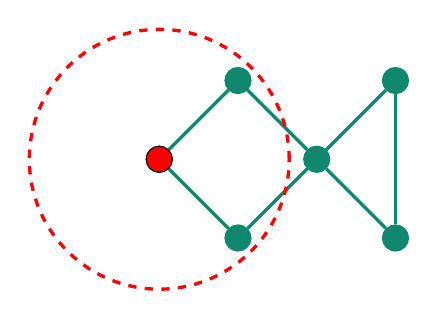
\begin{tikzpicture}
            \node[fill=PineGreen, PineGreen,draw, circle] (n1) at (0,0) {};
            \node[draw, circle,fill=red] (n1) at (0,0) {};
            \node[fill=PineGreen, PineGreen,draw, circle] (n2) at (1,1) {};
            \node[fill=PineGreen, PineGreen,draw, circle] (n4) at (1,-1) {};
            \node[fill=PineGreen, PineGreen,draw, circle] (n3) at (2,0) {};
            \node[fill=PineGreen, PineGreen,draw, circle] (n5) at (3,-1) {};
            \node[fill=PineGreen, PineGreen,draw, circle] (n6) at (3,1) {};

            \draw[very thick, fill=PineGreen, PineGreen,-] (n1)--(n2);
            \draw[very thick, fill=PineGreen, PineGreen,-] (n2)--(n3)--(n4);
            \draw[very thick, fill=PineGreen, PineGreen,-] (n4)--(n1);
            \draw[very thick, fill=PineGreen, PineGreen,-] (n3)--(n6);
            \draw[very thick, fill=PineGreen, PineGreen,-] (n6)--(n5);
            \draw[very thick, fill=PineGreen, PineGreen,-] (n5)--(n3);
            \draw[very thick, red, dashed, very thick] (0,0) circle (1.65);
        \end{tikzpicture}
    \end{center}
 Algorithm behaviors:

 \hspace{2cm}graph transformation according to 
\begin{tikzpicture}[baseline=-1ex]
            \node () at (0,0) {\text{local}};
            \draw[red, dashed, very thick] (0,0) circle (0.5);
        \end{tikzpicture} knowledge  

    \note{
On utilise les systèmes de transformation de graphes pour modéliser les systèmes distribués:

Une configuration du système est représentée par un graphe, où les nœuds représentent les unités de calcul et les arêtes représentent les canaux de communication entre ces unités.

Un comportement du système est représenté par une transformation de graphe en fonction de la connaissance locale de certain noeuds.

1m
    }
\end{frame}

\begin{frame}{Graph Transformation}
    Graph transformation rule:
        \begin{center}
        \resizebox{0.7\textwidth}{!}{
            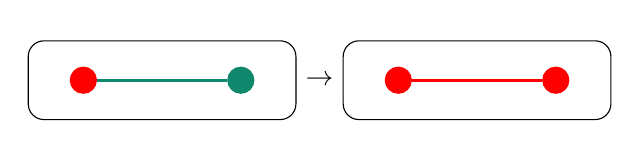
\begin{tikzpicture}
                        \graphbox{\(\)}{0mm}{0mm}{34mm}{10mm}{-10mm}{-5mm}{
                            \node[red,fill=red,draw, circle] (x) at (0,0) {};
                            \node () at (0,0.55) {};  
                            \node[PineGreen,fill=PineGreen,draw, circle] (y) at (2,0) {};
                            \node () at (2,0.55) {};
                            \draw[very thick, PineGreen,-] (x) -- node[midway,above] {} (y) ;
                            %             \draw[->] (x) edge [loop above] node {$A$} (x);
                            % \draw[->] (y) edge [loop above] node {$N$} (y);
                        }
                        \graphbox{\(\)}{40mm}{0mm}{34mm}{10 mm}{-10mm}{-5mm}{
                            \node[red,fill=red,draw, circle]  (x) at (0,0) {};  
                            \node () at (0,0.55) {};  
                            \node[red,fill=red,draw, circle]  (y) at (2,0) {};
                            \node () at (2,0.55) {};
                            \draw[very thick, red,-] (x) -- node[midway,above] {} (y) ;
                            % \draw[->] (x) edge [loop above] node {$A$} (x);
                            % \draw[->] (y) edge [loop above] node {$A$} (y);
                        }  
                        \node () at (37mm,-5mm) {\( \mathop{\rightarrow} \)}; % K -> L
            \end{tikzpicture}
        } 
        \end{center}
        Replace the left-hand side by the right-hand side.
        \newline\newline
        Spanning-tree construction:
%  \only<1-11>{Configuration of a distributed system:}
%  \only<12->{A spanning tree is obtained when the rule cannot be applied:}
    \begin{overlayarea}{\textwidth}{\textheight}
        \begin{center}
            \begin{onlyenv}<1>
            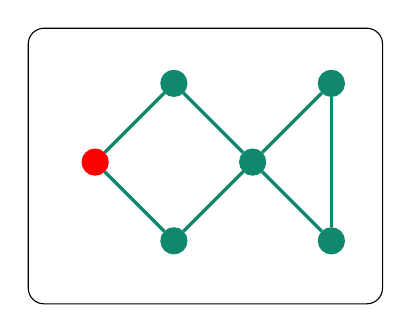
\begin{tikzpicture}
            \graphbox{}{0mm}{0mm}{45mm}{35mm}{-14mm}{-17mm}{
            \node[red,fill=red,draw, circle] (n1) at (0,0) {};
            \node[PineGreen,fill=PineGreen,draw, circle] (n2) at (1,1) {};
            \node[PineGreen,fill=PineGreen,draw, circle] (n3) at (2,0) {};
            \node[PineGreen,fill=PineGreen,draw, circle] (n4) at (1,-1) {};
            \node[PineGreen,fill=PineGreen,draw, circle] (n5) at (3,-1) {};
            \node[PineGreen,fill=PineGreen,draw, circle] (n6) at (3,1) {};
            \draw[very thick, PineGreen,-] (n1)-- node[pos=0.6, left] {} (n2);
            \draw[very thick, PineGreen,-] (n2)-- node[pos=0.35,right] {} (n3);
            \draw[very thick, PineGreen,-] (n3)-- node[pos=0.6,right] {}(n4);
            \draw[very thick, PineGreen,-] (n4)-- node[pos=0.45,left] {}(n1);
            \draw[very thick, PineGreen,-] (n3)-- node[pos=0.65,left] {}(n6);
            \draw[very thick, PineGreen,-] (n6)-- node[pos=0.4,right] {}(n5);
            \draw[very thick, PineGreen,-] (n5)-- node[pos=0.4,left] {}(n3);
            }
        \end{tikzpicture}
        % } 
        \end{onlyenv}
        \begin{onlyenv}<2>
               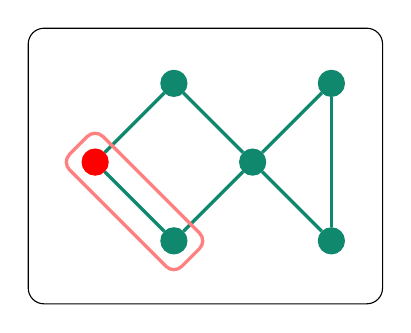
\begin{tikzpicture}
            \graphbox{}{0mm}{0mm}{45mm}{35mm}{-14mm}{-17mm}{
            \node[red,fill=red,draw, circle] (n1) at (0,0) {};
            \node[PineGreen,fill=PineGreen,draw, circle] (n2) at (1,1) {};
            \node[PineGreen,fill=PineGreen,draw, circle] (n3) at (2,0) {};
            \node[PineGreen,fill=PineGreen,draw, circle] (n4) at (1,-1) {};
            \node[PineGreen,fill=PineGreen,draw, circle] (n5) at (3,-1) {};
            \node[PineGreen,fill=PineGreen,draw, circle] (n6) at (3,1) {};
            \draw[very thick, PineGreen,-] (n1)-- node[pos=0.6, left] {} (n2);
            \draw[very thick, PineGreen,-] (n2)-- node[pos=0.35,right] {} (n3);
            \draw[very thick, PineGreen,-] (n3)-- node[pos=0.6,right] {}(n4);
            \draw[very thick, PineGreen,-] (n4)-- node[pos=0.45,left] {}(n1);
            \draw[very thick, PineGreen,-] (n3)-- node[pos=0.65,left] {}(n6);
            \draw[very thick, PineGreen,-] (n6)-- node[pos=0.4,right] {}(n5);
            \draw[very thick, PineGreen,-] (n5)-- node[pos=0.4,left] {}(n3);
             \draw[very thick, red!50, rounded corners,rotate around={45:(0,-0.5)}] ($(n4)+(-0.3,-0.3)$) rectangle ($(n1)+(0.3,0.3)$); 
            }
        \end{tikzpicture}
        \end{onlyenv}
         \begin{onlyenv}<3>
               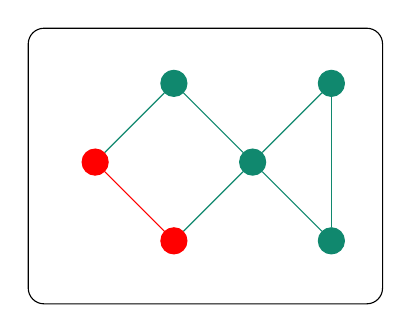
\begin{tikzpicture}
            \graphbox{}{0mm}{0mm}{45mm}{35mm}{-14mm}{-17mm}{
            \node[red,fill=red,draw, circle] (n1) at (0,0) {};
            \node[PineGreen,fill=PineGreen,draw, circle] (n2) at (1,1) {};
            \node[PineGreen,fill=PineGreen,draw, circle] (n3) at (2,0) {};
            \node[red,fill=red,draw, circle] (n4) at (1,-1) {};
            \node[PineGreen,fill=PineGreen,draw, circle] (n5) at (3,-1) {};
            \node[PineGreen,fill=PineGreen,draw, circle] (n6) at (3,1) {};
            \draw[PineGreen,-] (n1)-- node[pos=0.6, left] {} (n2);
            \draw[PineGreen,-] (n2)-- node[pos=0.35,right] {} (n3);
            \draw[PineGreen,-] (n3)-- node[pos=0.6,right] {}(n4);
            \draw[red,-] (n4)-- node[pos=0.45,left] {}(n1);
            \draw[PineGreen,-] (n3)-- node[pos=0.65,left] {}(n6);
            \draw[PineGreen,-] (n6)-- node[pos=0.4,right] {}(n5);
            \draw[PineGreen,-] (n5)-- node[pos=0.4,left] {}(n3);
            }
        \end{tikzpicture}
        \end{onlyenv}
        \begin{onlyenv}<4>
               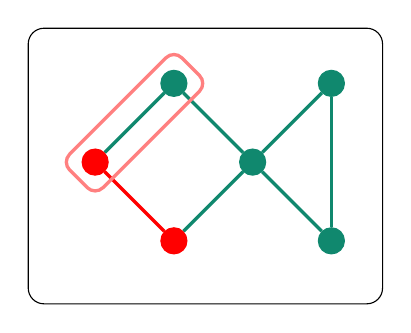
\begin{tikzpicture}
            \graphbox{}{0mm}{0mm}{45mm}{35mm}{-14mm}{-17mm}{
            \node[red,fill=red,draw, circle] (n1) at (0,0) {};
            \node[PineGreen,fill=PineGreen,draw, circle] (n2) at (1,1) {};
            \node[PineGreen,fill=PineGreen,draw, circle] (n3) at (2,0) {};
            \node[red,fill=red,draw, circle] (n4) at (1,-1) {};
            \node[PineGreen,fill=PineGreen,draw, circle] (n5) at (3,-1) {};
            \node[PineGreen,fill=PineGreen,draw, circle] (n6) at (3,1) {};
            \draw[very thick, PineGreen,-] (n1)-- node[pos=0.6, left] {} (n2);
            \draw[very thick, PineGreen,-] (n2)-- node[pos=0.35,right] {} (n3);
            \draw[very thick, PineGreen,-] (n3)-- node[pos=0.6,right] {}(n4);
            \draw[very thick, red,-] (n4)-- node[pos=0.45,left] {}(n1);
            \draw[very thick, PineGreen,-] (n3)-- node[pos=0.65,left] {}(n6);
            \draw[very thick, PineGreen,-] (n6)-- node[pos=0.4,right] {}(n5);
            \draw[very thick, PineGreen,-] (n5)-- node[pos=0.4,left] {}(n3);
            \draw[very thick, red!50, rounded corners,rotate around={45:(0,-0.5)}] ($(n1)+(-0.3,-0.3)$) rectangle ($(n2)+(0.3,0.3)$); 
            }
        \end{tikzpicture}
        \end{onlyenv}
        \begin{onlyenv}<5>
               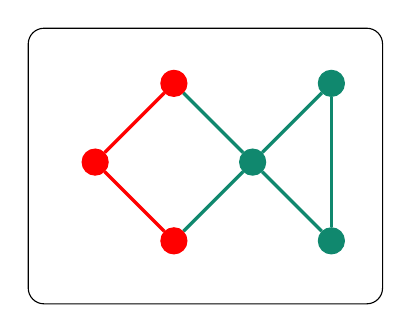
\begin{tikzpicture}
            \graphbox{}{0mm}{0mm}{45mm}{35mm}{-14mm}{-17mm}{
            \node[red,fill=red,draw, circle] (n1) at (0,0) {};
            \node[red,fill=red,draw, circle] (n2) at (1,1) {};
            \node[PineGreen,fill=PineGreen,draw, circle] (n3) at (2,0) {};
            \node[red,fill=red,draw, circle] (n4) at (1,-1) {};
            \node[PineGreen,fill=PineGreen,draw, circle] (n5) at (3,-1) {};
            \node[PineGreen,fill=PineGreen,draw, circle] (n6) at (3,1) {};
            \draw[very thick, red,-] (n1)-- node[pos=0.6, left] {} (n2);
            \draw[very thick, PineGreen,-] (n2)-- node[pos=0.35,right] {} (n3);
            \draw[very thick, PineGreen,-] (n3)-- node[pos=0.6,right] {}(n4);
            \draw[very thick, red,-] (n4)-- node[pos=0.45,left] {}(n1);
            \draw[very thick, PineGreen,-] (n3)-- node[pos=0.65,left] {}(n6);
            \draw[very thick, PineGreen,-] (n6)-- node[pos=0.4,right] {}(n5);
            \draw[very thick, PineGreen,-] (n5)-- node[pos=0.4,left] {}(n3);
            }
        \end{tikzpicture}
        \end{onlyenv}
        \begin{onlyenv}<6>
               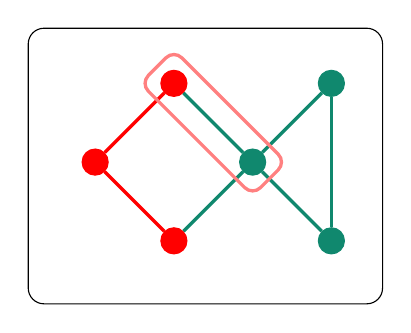
\begin{tikzpicture}
            \graphbox{}{0mm}{0mm}{45mm}{35mm}{-14mm}{-17mm}{
            \node[red,fill=red,draw, circle] (n1) at (0,0) {};
            \node[red,fill=red,draw, circle] (n2) at (1,1) {};
            \node[PineGreen,fill=PineGreen,draw, circle] (n3) at (2,0) {};
            \node[red,fill=red,draw, circle] (n4) at (1,-1) {};
            \node[PineGreen,fill=PineGreen,draw, circle] (n5) at (3,-1) {};
            \node[PineGreen,fill=PineGreen,draw, circle] (n6) at (3,1) {};
            \draw[very thick, red,-] (n1)-- node[pos=0.6, left] {} (n2);
            \draw[very thick, PineGreen,-] (n2)-- node[pos=0.35,right] {} (n3);
            \draw[very thick, PineGreen,-] (n3)-- node[pos=0.6,right] {}(n4);
            \draw[very thick, red,-] (n4)-- node[pos=0.45,left] {}(n1);
            \draw[very thick, PineGreen,-] (n3)-- node[pos=0.65,left] {}(n6);
            \draw[very thick, PineGreen,-] (n6)-- node[pos=0.4,right] {}(n5);
            \draw[very thick, PineGreen,-] (n5)-- node[pos=0.4,left] {}(n3);
            \draw[very thick, red!50, rounded corners,rotate around={45:(0.5,0.5)}] ($(n3)+(-0.3,-0.3)$) rectangle ($(n2)+(0.3,0.3)$); 
            }
        \end{tikzpicture}
        \end{onlyenv}
         \begin{onlyenv}<7>
               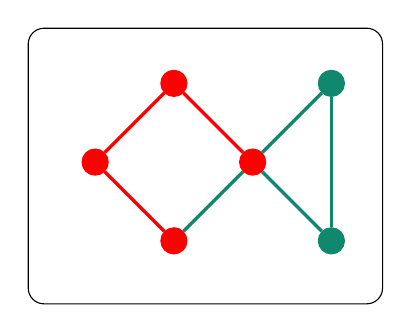
\begin{tikzpicture}
            \graphbox{}{0mm}{0mm}{45mm}{35mm}{-14mm}{-17mm}{
            \node[red,fill=red,draw, circle] (n1) at (0,0) {};
            \node[red,fill=red,draw, circle] (n2) at (1,1) {};
            \node[red,fill=red,draw, circle] (n3) at (2,0) {};
            \node[red,fill=red,draw, circle] (n4) at (1,-1) {};
            \node[PineGreen,fill=PineGreen,draw, circle] (n5) at (3,-1) {};
            \node[PineGreen,fill=PineGreen,draw, circle] (n6) at (3,1) {};
            \draw[very thick, red,-] (n1)-- node[pos=0.6, left] {} (n2);
            \draw[very thick, red,-] (n2)-- node[pos=0.35,right] {} (n3);
            \draw[very thick, PineGreen,-] (n3)-- node[pos=0.6,right] {}(n4);
            \draw[very thick, red,-] (n4)-- node[pos=0.45,left] {}(n1);
            \draw[very thick, PineGreen,-] (n3)-- node[pos=0.65,left] {}(n6);
            \draw[very thick, PineGreen,-] (n6)-- node[pos=0.4,right] {}(n5);
            \draw[very thick, PineGreen,-] (n5)-- node[pos=0.4,left] {}(n3);
            }
        \end{tikzpicture}
        \end{onlyenv}
         \begin{onlyenv}<8>
               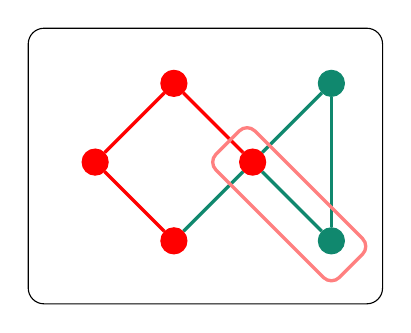
\begin{tikzpicture}
            \graphbox{}{0mm}{0mm}{45mm}{35mm}{-14mm}{-17mm}{
            \node[red,fill=red,draw, circle] (n1) at (0,0) {};
            \node[red,fill=red,draw, circle] (n2) at (1,1) {};
            \node[red,fill=red,draw, circle] (n3) at (2,0) {};
            \node[red,fill=red,draw, circle] (n4) at (1,-1) {};
            \node[PineGreen,fill=PineGreen,draw, circle] (n5) at (3,-1) {};
            \node[PineGreen,fill=PineGreen,draw, circle] (n6) at (3,1) {};
            \draw[very thick, red,-] (n1)-- node[pos=0.6, left] {} (n2);
            \draw[very thick, red,-] (n2)-- node[pos=0.35,right] {} (n3);
            \draw[very thick, PineGreen,-] (n3)-- node[pos=0.6,right] {}(n4);
            \draw[very thick, red,-] (n4)-- node[pos=0.45,left] {}(n1);
            \draw[very thick, PineGreen,-] (n3)-- node[pos=0.65,left] {}(n6);
            \draw[very thick, PineGreen,-] (n6)-- node[pos=0.4,right] {}(n5);
            \draw[very thick, PineGreen,-] (n5)-- node[pos=0.4,left] {}(n3);
            % \draw[red!50, rounded corners,rotate around={45:(1.5,0.5)}] ($(n3)+(-0.3,-0.3)$) rectangle ($(n6)+(0.3,0.3)$); 
            \draw[very thick, red!50, rounded corners,rotate around={45:(1.5,0.5)}] ($(n5)+(-0.4,-0.4)$) rectangle ($(n3)+(0.3,0.4)$); 
            }
        \end{tikzpicture}
        \end{onlyenv}
        \begin{onlyenv}<9>
            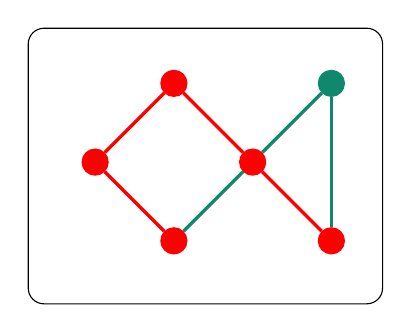
\begin{tikzpicture}
            \graphbox{}{0mm}{0mm}{45mm}{35mm}{-14mm}{-17mm}{
              \node[red,fill=red,draw, circle] (n1) at (0,0) {};
              \node[red,fill=red,draw, circle] (n2) at (1,1) {};
              \node[red,fill=red,draw, circle] (n3) at (2,0) {};
              \node[red,fill=red,draw, circle] (n4) at (1,-1) {};
              \node[red,fill=red,draw, circle] (n5) at (3,-1) {};
              \node[PineGreen,fill=PineGreen,draw, circle] (n6) at (3,1) {};
              \draw[very thick, red,-] (n1)-- node[pos=0.6, left] {} (n2);
              \draw[very thick, red,-] (n2)-- node[pos=0.35,right] {} (n3);
              \draw[very thick, PineGreen,-] (n3)-- node[pos=0.6,right] {}(n4);
              \draw[very thick, red,-] (n4)-- node[pos=0.45,left] {}(n1);
              \draw[very thick, PineGreen,-] (n3)-- node[pos=0.65,left] {}(n6);
              \draw[very thick, PineGreen,-] (n6)-- node[pos=0.4,right] {}(n5);
              \draw[very thick, red,-] (n5)-- node[pos=0.4,left] {}(n3);
              }
          \end{tikzpicture}
        \end{onlyenv}
         \begin{onlyenv}<10>
               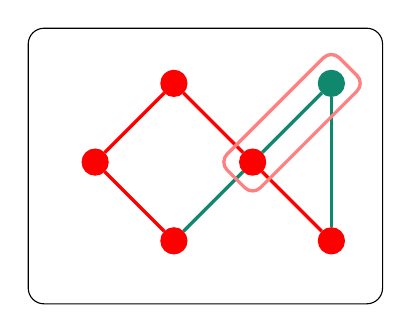
\begin{tikzpicture}
            \graphbox{}{0mm}{0mm}{45mm}{35mm}{-14mm}{-17mm}{
              \node[red,fill=red,draw, circle] (n1) at (0,0) {};
              \node[red,fill=red,draw, circle] (n2) at (1,1) {};
              \node[red,fill=red,draw, circle] (n3) at (2,0) {};
              \node[red,fill=red,draw, circle] (n4) at (1,-1) {};
              \node[red,fill=red,draw, circle] (n5) at (3,-1) {};
              \node[PineGreen,fill=PineGreen,draw, circle] (n6) at (3,1) {};
              \draw[very thick, red,-] (n1)-- node[pos=0.6, left] {} (n2);
              \draw[very thick, red,-] (n2)-- node[pos=0.35,right] {} (n3);
              \draw[very thick, PineGreen,-] (n3)-- node[pos=0.6,right] {}(n4);
              \draw[very thick, red,-] (n4)-- node[pos=0.45,left] {}(n1);
              \draw[very thick, PineGreen,-] (n3)-- node[pos=0.65,left] {}(n6);
              \draw[very thick, PineGreen,-] (n6)-- node[pos=0.4,right] {}(n5);
              \draw[very thick, red,-] (n5)-- node[pos=0.4,left] {}(n3);
              \draw[very thick, red!50, rounded corners,rotate around={45:(1.5,0.5)}] ($(n3)+(-0.3,-0.3)$) rectangle ($(n6)+(0.3,0.3)$); 
              % \draw[red!50, rounded corners,rotate around={45:(1.5,0.5)}] ($(n5)+(-0.4,-0.4)$) rectangle ($(n3)+(0.3,0.4)$); 
            }
        \end{tikzpicture}
        \end{onlyenv}
        \begin{onlyenv}<11>
               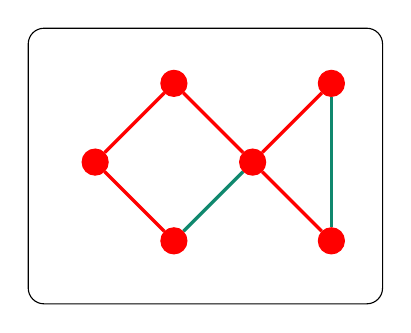
\begin{tikzpicture}
            \graphbox{}{0mm}{0mm}{45mm}{35mm}{-14mm}{-17mm}{
            \node[red,fill=red,draw, circle] (n1) at (0,0) {};
            \node[red,fill=red,draw, circle] (n2) at (1,1) {};
            \node[red,fill=red,draw, circle] (n3) at (2,0) {};
            \node[red,fill=red,draw, circle] (n4) at (1,-1) {};
            \node[red,fill=red,draw, circle] (n5) at (3,-1) {};
            \node[red,fill=red,draw, circle] (n6) at (3,1) {};
            \draw[very thick, red,-] (n1)-- node[pos=0.6, left] {} (n2);
            \draw[very thick, red,-] (n2)-- node[pos=0.35,right] {} (n3);
            \draw[very thick, PineGreen,-] (n3)-- node[pos=0.6,right] {}(n4);
            \draw[very thick, red,-] (n4)-- node[pos=0.45,left] {}(n1);
            \draw[very thick, red,-] (n3)-- node[pos=0.65,left] {}(n6);
            \draw[very thick, PineGreen,-] (n6)-- node[pos=0.4,right] {}(n5);
            \draw[very thick, red,-] (n5)-- node[pos=0.4,left] {}(n3);
            }
        \end{tikzpicture}
        \end{onlyenv}
          \begin{onlyenv}<12->
               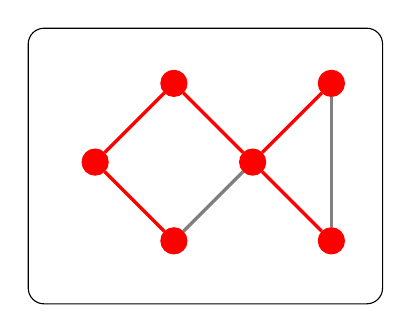
\begin{tikzpicture}
            \graphbox{}{0mm}{0mm}{45mm}{35mm}{-14mm}{-17mm}{
            \node[red,fill=red,draw, circle] (n1) at (0,0) {};
            \node[red,fill=red,draw, circle] (n2) at (1,1) {};
            \node[red,fill=red,draw, circle] (n3) at (2,0) {};
            \node[red,fill=red,draw, circle] (n4) at (1,-1) {};
            \node[red,fill=red,draw, circle] (n5) at (3,-1) {};
            \node[red,fill=red,draw, circle] (n6) at (3,1) {};
            \draw[very thick, red,-] (n1)-- node[pos=0.6, left] {} (n2);
            \draw[very thick, red,-] (n2)-- node[pos=0.35,right] {} (n3);
            \draw[very thick, gray,-] (n3)-- node[pos=0.6,right] {}(n4);
            \draw[very thick, red,-] (n4)-- node[pos=0.45,left] {}(n1);
            \draw[very thick, red,-] (n3)-- node[pos=0.65,left] {}(n6);
            \draw[very thick, gray,-] (n6)-- node[pos=0.4,right] {}(n5);
            \draw[very thick, red,-] (n5)-- node[pos=0.4,left] {}(n3);
            }
        \end{tikzpicture}
        \end{onlyenv}
     \end{center}

    \begin{onlyenv}<12->
          \textcolor{PineGreen}{A spanning tree is obtained when the rule cannot be applied.}
    \end{onlyenv} 
        \begin{onlyenv}<13->
          \textcolor{red}{Does the transformation process terminate for any initial graph?}
            % \textcolor{red}{Does the transformation process terminate for any initial graph under the strategy of applying the rule while possible?}
        \end{onlyenv} 
    \end{overlayarea}
    
    \note{The graph models a distributed network of six computational units.
Each node represents a computational unit; a node's state is indicated by the label of its self-loop; each edge represents a communication channel. node $1$ labeled by $A$ represents an active computational unit, the other nodes labeled by $N$ represent neutral computational units, and edges labeled by $0$ represent communication channels in state $0$.}

\note{with each others

behavior is difficult

}
\note{
Une regle de transformation de graphes est donnee par deux graphes separes par une fleche. Elle remplace une occurrence du graphe de gauche par celle de droite.
 
On peut appliquer cette regle pour construire un arbre couvrant du graphe en bas. 
A chaque etape, on cherche une occurrence du graphe de gauche dans le graphe courant, puis on la remplace par le graphe de droite.
Quand on ne peut plus appliquer la regle, on obtient un arbre couvrant avec les aretes rouges.

Une question importante est de savoir si le processus de transformation termine pour n'importe quel graphe initial.

1m30
}
\end{frame}


\begin{frame}{Termination of Graph Transformation Systems}
  \begin{itemize}
    \item No graph $G_0$ can be transformed forever
         $$G_0 \Rightarrow G_1 \Rightarrow \cdots$$
        %  under the strategy 
        %   \begin{center}
        %       \textcolor{blue}{\enquote{apply rules as long as possible}}
        %   \end{center}
    \item Aligns with the notion of program termination: 
         \begin{center}
            \textcolor{blue}{\enquote{every execution (on any input) halts.}}
          \end{center}
    \item Undecidable in general~\cite{plump1995ontermination}
       \begin{itemize}
        \item Automated techniques for specific subclasses
       \end{itemize}
  \end{itemize}
    \note{
La terminaison d'un système de transformation de graphes signifie qu'il n'existe pas de graphe initial qui peut être transformé indéfiniment.

Cette notion coïncide avec la terminaison des programmes, qui signifie que chaque exécution sur n'importe quelle entrée s'arrête.

La terminaison des systèmes de transformation de graphes est indécidable en général. 
Cependant, il existe des techniques automatisées pour des sous-classes spécifiques.

1m
}
\end{frame}

\begin{frame}{Termination by interpretations~\cite{zantema2014termination,nipkow1998term}}
    \begin{beamercolorbox}[rounded=true,shadow=true,wd=\textwidth]{block body}
        % Termination by interpretations:
        \begin{description}
            \item[Interpret graphs as natural numbers.]
            \item[Show each transformation step strictlydecreases the value.]
        \end{description}
    \end{beamercolorbox}

    % \begin{center}
\noindent   Number of edges: 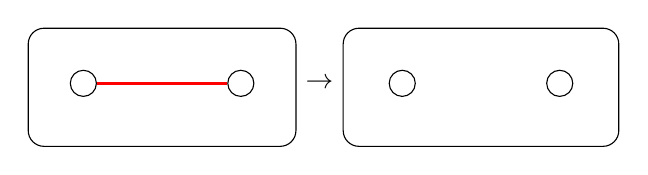
\begin{tikzpicture}[baseline=-12mm]
                    \graphbox{}{0mm}{-3mm}{34mm}{15mm}{0mm}{4mm}{
                        \coordinate (o) at (0mm,-11mm); 
                        \node[draw,circle] (l1) at ($(o)+(-10mm,0mm)$) {};
                        \node[draw,circle] (l2) at ($(l1)+(2,0)$) {};
                        % \node[draw,circle] (l3) at ($(l1)+(1,0)$) {3};
                        \draw[very thick, red,-] (l1) -- (l2) node[midway,above] {};
                    } 
                    % \graphbox{\( K \)}{40mm}{-3mm}{34mm}{15mm}{2mm}{2mm}{
                    %     \coordinate (o) at (0mm,-11mm); 
                    %     \node[draw,circle] (l1) at ($(o)+(-10mm,0mm)$) {1};
                    %     \node[draw,circle] (l2) at ($(l1)+(2,0)$) {2};
                    % }  
                    \graphbox{}{40mm}{-3mm}{35mm}{15mm}{5mm}{4mm}{
                        \coordinate (o) at (-5mm,-11mm); 
                        \node[draw,circle] (l1) at ($(o)+(-10mm,0mm)$) {};
                        % \node[draw,circle] (l2) at ($(l1)+(3,0)$) {2};
                         % \node[draw,circle] (l3) at ($(l1)+(1,0)$) {4};
                        \node[draw,circle] (l4) at ($(l1)+(2,0)$) {};
                        % \draw[->] (l1) -- (l4) node[midway,above] {};
                        % \draw[->] (l4) -- (l2) node[midway,above] {$a$};
                    }    
                    \node () at (37mm,-10mm) {\( \rightarrow \)}; % K -> L
                    % \node () at (77mm,-10mm) {\( \rightarrow \)}; % K -> R
                \end{tikzpicture}
    % \end{center}
    % \begin{center}


     \noindent  Number of nodes: 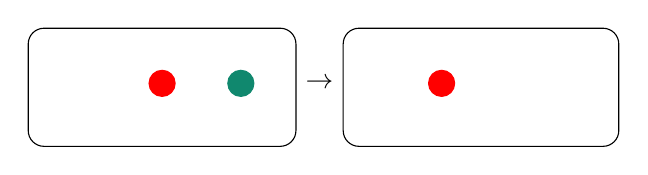
\begin{tikzpicture}[baseline=-12mm]
                    \graphbox{}{0mm}{-3mm}{34mm}{15mm}{0mm}{4mm}{
                        \coordinate (o) at (0mm,-11mm); 
                        \node[fill=red,red,draw,circle] (l1) at ($(o)+(0mm,0mm)$) {};
                        \node[fill=PineGreen,PineGreen,draw,circle] (l3) at ($(l1)+(1,0)$) {};
                    } 
                    % \graphbox{\( K \)}{40mm}{-3mm}{34mm}{15mm}{2mm}{2mm}{
                    %     \coordinate (o) at (0mm,-11mm); 
                    %     \node[draw,circle] (l1) at ($(o)+(-10mm,0mm)$) {1};
                    %     \node[draw,circle] (l2) at ($(l1)+(2,0)$) {2};
                    % }  
                    \graphbox{}{40mm}{-3mm}{35mm}{15mm}{5mm}{4mm}{
                        \coordinate (o) at (0mm,-11mm); 
                        \node[fill=red,red,draw,circle] (l1) at ($(o)+(-10mm,0mm)$) {};
                    }    
                    \node () at (37mm,-10mm) {\( \rightarrow \)}; % K -> L
                    % \node () at (77mm,-10mm) {\( \rightarrow \)}; % K -> R
                \end{tikzpicture}
    % \end{center}


    \vspace{3mm}
      \noindent Number of edges labeled by $a$: 
    \begin{center}
       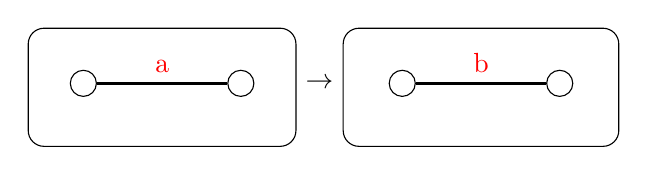
\begin{tikzpicture}
                    \graphbox{}{0mm}{-3mm}{34mm}{15mm}{0mm}{4mm}{
                        \coordinate (o) at (0mm,-11mm); 
                        \node[draw,circle] (l1) at ($(o)+(-10mm,0mm)$) {};
                        \node[draw,circle] (l2) at ($(l1)+(2,0)$) {};
                        % \node[draw,circle] (l3) at ($(l1)+(1,0)$) {3};
                        \draw[very thick, -] (l1) -- (l2) node[midway,above] {\textcolor{red}{a}};
                    } 
                    % \graphbox{\( K \)}{40mm}{-3mm}{34mm}{15mm}{2mm}{2mm}{
                    %     \coordinate (o) at (0mm,-11mm); 
                    %     \node[draw,circle] (l1) at ($(o)+(-10mm,0mm)$) {1};
                    %     \node[draw,circle] (l2) at ($(l1)+(2,0)$) {2};
                    % }  
                    \graphbox{}{40mm}{-3mm}{35mm}{15mm}{5mm}{4mm}{
                        \coordinate (o) at (-5mm,-11mm); 
                        \node[draw,circle] (l1) at ($(o)+(-10mm,0mm)$) {};
                        % \node[draw,circle] (l2) at ($(l1)+(3,0)$) {2};
                         % \node[draw,circle] (l3) at ($(l1)+(1,0)$) {4};
                        \node[draw,circle] (l4) at ($(l1)+(2,0)$) {};
                        \draw[very thick, -] (l1) -- (l4) node[midway,above] {\textcolor{red}{b}};
                        % \draw[->] (l4) -- (l2) node[midway,above] {$a$};
                    }    
                    \node () at (37mm,-10mm) {\( \rightarrow \)}; % K -> L
                    % \node () at (77mm,-10mm) {\( \rightarrow \)}; % K -> R
                \end{tikzpicture}
    \end{center}
   
    \note{
    Une façon de prouver la terminaison est d'interpreter les graphes par des entiers naturels, et de montrer que chaque etape de transformation diminue la valeur.

    Par example, la premiere règle diminue le nombre d'aretes, la deuxieme diminue le nombre de noeuds, et la troisieme diminue le nombre d'aretes étiquetées par a. Leur terminaison peut être prouvée en interpretant les graphes par le nombre d'aretes, de noeuds, et d'aretes étiquetées par a, respectivement.

    1m
    }

\end{frame}
\begin{frame}{Limitation}
    \begin{center}
      \resizebox{\textwidth}{!}{
       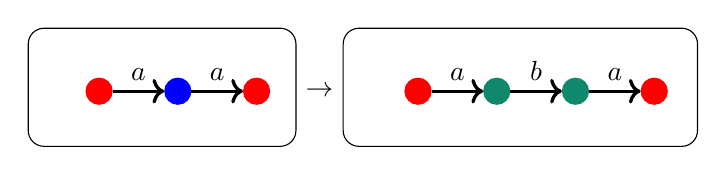
\begin{tikzpicture}[baseline=-10mm]
          \graphbox{}{0mm}{0mm}{34mm}{15mm}{2mm}{-5mm}{
              \coordinate (o) at (0mm,-3mm); 
              \node[draw,circle,red,fill=red] (l1) at ($(o)+(-10mm,0mm)$) {};
              \node[draw,circle,red,fill=red] (l2) at ($(l1)+(2,0)$) {};
              \node[draw,circle,blue,fill=blue] (l3) at ($(l1)+(1,0)$) {};
              \draw[very thick, ->] (l1) -- (l3) node[midway,above] {$a$};
              \draw[very thick, ->] (l3) -- (l2) node[midway,above] {$a$};
          }     
          \graphbox{}{40mm}{0mm}{45mm}{15mm}{2mm}{-5mm}{
              \coordinate (o) at (-5mm,-3mm); 
              \node[draw,circle,red,fill=red] (l1) at ($(o)+(-10mm,0mm)$) {};
              \node[draw,circle,red,fill=red] (l2) at ($(l1)+(3,0)$) {};
              \node[draw,circle,PineGreen,fill=PineGreen] (l3) at ($(l1)+(1,0)$) {};
              \node[draw,circle,PineGreen,fill=PineGreen] (l4) at ($(l1)+(2,0)$) {};
              \draw[very thick, ->] (l1) -- (l3) node[midway,above] {$a$};
              \draw[very thick, ->] (l3) -- (l4) node[midway,above] {$b$};
              \draw[very thick, ->] (l4) -- (l2) node[midway,above] {$a$};
          }    
          \node () at (37mm,-8mm) {$\rightarrow$};
          % \draw[>->] (51mm,2mm) -- (52mm,3mm);
      \end{tikzpicture}
      }
  \end{center} 

  \begin{description}
      \item[Number of nodes/edges/labels do not decrease.]
    % \item[Left-hand side graph:] middle has no other incident edges
    % \item[Right-hand side graph:] middles are fresh nodes
    % \item[\noindent Termination:] number of \raisebox{2pt}{
    %         \scalebox{0.7}{\tikz[baseline=-0.5ex]{
    %         \node [draw,circle] (z) at (-1,0) {};
    %         \node [draw,circle] (x) at (0,0) {};
    %         \node[draw,circle] (y) at (1,0) {};
    %         \draw[->] (z)--(x) node[midway, above] {$a$};
    %         \draw[->] (x)--(y) node[midway, above] {$a$};
    %     }}} decreases
    \item[Can its termination be proved by interpretations?]\ \\
      \begin{itemize}
        % \item Weighted Type Graph Method
        \item Need a formal definition of graph transformations.
      \end{itemize}
  \end{description}
  \note{
Cette règle de transformation ne diminue ni le nombre de noeuds, ni le nombre d'aretes, ni le nombre d'aretes étiquetées par a ou b. 
Peut-on prouver sa terminaison par une interprétation?
Afin de répondre à cette question, nous avons besoin d'une définition formelle des transformations de graphes.

30s
% 8s + 1m30 + 1m + 1m30 + 1m + 1m + 30s = 6m38s
  }

\end{frame}

\begin{frame}{Structure of the Remainder}
    \tableofcontents
    \note{
    Le reste de la présentation est structuré comme suit:
    Tout d'abord, nous présentons une définition formelle des transformations de graphes.
    Ensuite, nous présentons une contribution qui améliore l'utilisabilité d'une technique existante. 
    Et puis, nous présentons notre contribution principale: une nouvelle technique de terminaison.
    Enfin, nous présentons un outil qui implante nos contributions
    avant de conclure.
    1m
    }
\end{frame}

\begin{frame}{Graph Morphisms: Structure-Preserving Functions}
             \begin{center}
          \resizebox{0.7\textwidth}{!}{
        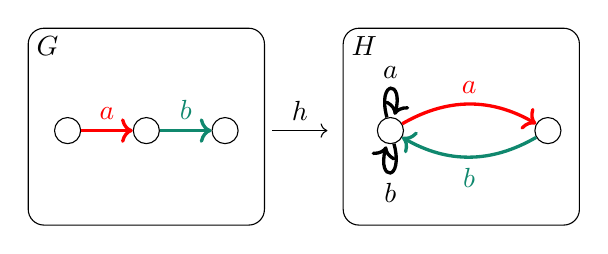
\begin{tikzpicture}
          \graphbox{$G$}{-40mm}{0mm}{30mm}{25mm}{0mm}{-3mm}{
            \coordinate (o) at (0mm,-10mm); 
            \node[draw,circle] (l1) at ($(o)+(-10mm,0mm)$) {};
            \node[draw,circle] (l2) at ($(l1)+(2,0)$) {};
            \node[draw,circle] (l3) at ($(l1)+(1,0)$) {};
            \draw[very thick, red,->] (l1) -- (l3) node[midway,above] {$a$};
            \draw[very thick, PineGreen,->] (l3) -- (l2) node[midway,above] {$b$};
        } 
            \graphbox{$H$}{0mm}{0mm}{30mm}{25mm}{-9mm}{-13mm}{
                \node[draw,circle] (1) at (0,0) {};
                \node[draw,circle] (2) at (2,0) {};
                \draw[very thick, ->] (1) edge[loop above] node[midway, above] {$a$} (1);
                \draw[very thick, ->] (1) edge[loop below] node[midway, below] {$b$} (1);
                \draw[very thick, ->,red] (1) edge[bend left] node[midway, above] {$a$}  (2);
                \draw[very thick, ->,PineGreen] (2) edge[bend left] node[midway, below] {$b$} (1);
            }
            % \node () at (-5mm,-15mm) {$\overset{h}{\to}$};
            \draw[->] (-9mm,-13mm) to node[midway,above] {$h$} (-2mm,-13mm);
        \end{tikzpicture}
          }
         \end{center}

    Colors show edge correspondence.
        \begin{center}
          \resizebox{0.7\textwidth}{!}{
        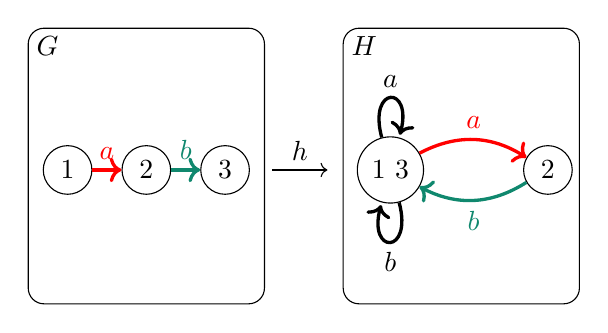
\begin{tikzpicture}
          \graphbox{$G$}{-40mm}{0mm}{30mm}{35mm}{0mm}{-8mm}{
            \coordinate (o) at (0mm,-10mm); 
            \node[draw,circle] (l1) at ($(o)+(-10mm,0mm)$) {1};
            \node[draw,circle] (l2) at ($(l1)+(2,0)$) {3};
            \node[draw,circle] (l3) at ($(l1)+(1,0)$) {2};
            \draw[very thick, red,->] (l1) -- (l3) node[midway,above] {$a$};
            \draw[very thick, PineGreen,->] (l3) -- (l2) node[midway,above] {$b$};
        } 
            \graphbox{$H$}{0mm}{0mm}{30mm}{35mm}{-9mm}{-18mm}{
                \node[draw,circle] (1) at (0,0) {1 3};
                \node[draw,circle] (2) at (2,0) {2};
                \draw[very thick, ->] (1) edge[loop above] node[midway, above] {$a$} (1);
                \draw[very thick, ->] (1) edge[loop below] node[midway, below] {$b$} (1);
                \draw[very thick, ->,red] (1) edge[bend left] node[midway, above] {$a$}  (2);
                \draw[very thick, ->,PineGreen] (2) edge[bend left] node[midway, below] {$b$} (1);
            }
            % \node () at (-5mm,-15mm) {$\overset{h}{\to}$};
            \draw[->] (-9mm,-18mm) to node[midway,above] {$h$} (-2mm,-18mm);
        \end{tikzpicture}
          }
         \end{center}

    Numbers show node correspondence.
    \note{
    Un morphisme de graphes est une fonction qui envoie les noeuds et les arêtes d'un graphe sur ceux d'un autre en respectant la structure des graphes.

    On utilise des couleurs pour montrer la correspondance des noeuds et des arêtes. 
    On utiliser aussi des numéros pour préciser la correspondance des noeuds.

    45s
    }
\end{frame}

\begin{frame}{Commutative Diagram}
    \begin{beamercolorbox}[rounded=true,shadow=true,wd=\textwidth]{block body}
        \begin{center}
            \resizebox{0.3\textwidth}{!}{
                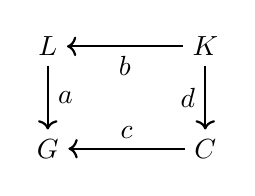
\begin{tikzpicture}
                    \node (I) at (0,-0.7) {$K$};
                    \node (L) at (-2,-0.7) {$L$};
                    \node (G) at (-2,-2) {$G$};
                    \node (C) at (0,-2) {$C$};
                    \draw [thick, ->] (I) to  node [midway,below] {$b$} (L);
                    \draw [thick, ->] (L) to node [midway,right] {$a$} (G);
                    \draw [thick, ->] (I) to node [midway,left] {$d$} (C);
                    \draw [thick, ->] (C) to node [midway,above] {$c$} (G);
                \end{tikzpicture}
            } 
        \end{center}
        commutes if \( a \circ b = c \circ d \).
    \end{beamercolorbox}
        
        \begin{center}
                \begin{tikzpicture}
                    \graphbox{}{0mm}{0mm}{34mm}{15mm}{2mm}{0mm}{
                        \coordinate (o) at (0mm,-8mm); 
                        \node[PineGreen,fill=PineGreen,circle] (l1) at ($(o)+(-10mm,0mm)$) {};
                        \node[red,fill=red,draw,circle] (l2) at ($(l1)+(2,0)$) {};
                        \node[draw,circle] (l3) at ($(l1)+(1,0)$) {};
                        \draw[very thick, ->] (l1) -- (l3) node[midway,above] {};
                        \draw[very thick, ->] (l3) -- (l2) node[midway,above] {};
                    } 
                    \graphbox{}{40mm}{0mm}{34mm}{15mm}{2mm}{0mm}{
                        \coordinate (o) at (0mm,-8mm); 
                        \node[PineGreen,fill=PineGreen,draw,circle] (l1) at ($(o)+(-10mm,0mm)$) {};
                        \node[red,fill=red,draw,circle] (l2) at ($(l1)+(2,0)$) {};
                    }  
                
                    \graphbox{ }{0mm}{-22mm}{34mm}{25mm}{2mm}{-5mm}{
                        \coordinate (o) at (0mm,-3mm); 
                        \node[PineGreen,fill=PineGreen,draw,circle] (l1) at ($(o)+(-10mm,0mm)$) {};
                        \node[red,fill=red,draw,circle] (l2) at ($(l1)+(2,0)$) {};
                        \node[draw,circle ] (l3) at ($(l1)+(1,0)$) {};
                        \node[blue,fill=blue,draw,circle] (l4) at ($(l2)+(0,-1)$) {};
                        \draw[very thick, ->] (l1) -- (l3) node[midway,above] {};
                        \draw[very thick, ->] (l3) -- (l2) node[midway,above] {};
                        \draw[very thick, ->] (l2) -- (l4) node[midway,right] {};
                    }    
                    \graphbox{ }{40mm}{-22mm}{34mm}{25mm}{2mm}{-5mm}{
                        \coordinate (o) at (0mm,-3mm); 
                        \node[PineGreen,fill=PineGreen,draw,circle] (l1) at ($(o)+(-10mm,0mm)$) {};
                        \node[red,fill=red,draw,circle] (l2) at ($(l1)+(2,0)$) {};
                        \node[blue,fill=blue,draw,circle] (l4) at ($(l2)+(0,-1)$) {};
                        \draw[very thick, ->] (l2) -- (l4) node[midway,right] {};
                    }    
                    \node () at (37mm,-8mm) {\( \underset{b}{\leftarrow} \)};  
                    \node () at (17mm,-18mm) {\( \downarrow\ a \)};
                    \node () at (37mm,-33mm) {\( \overset{c}{\leftarrow} \)};
                    \node () at (52mm,-18mm) {\( d\ \downarrow \)};
            \end{tikzpicture}
        \end{center}
    \note{
        Un diagramme des morphismes de graphes commute si pour n'importe quel chemin entre deux graphes, la composition des morphismes le long de ce chemin est la même.

        Par example, le rectangle KLGC commute si la composition de a et b est égale à la composition de c et d.

        45s
    }
\end{frame}

\begin{frame}{Pushouts: Gluing Graphs Along an Interface}
\begin{beamercolorbox}[rounded=true,shadow=true,wd=\textwidth]{block body}
    The \textbf{pushout} of \((\alpha,\beta) \)
    is  
        \( \textcolor{red}{(\beta',\alpha')}\) with
 
    \begin{itemize}
        \item $\square$\text{ABDC} commutes,
        \item<2->{universality:} \color{PineGreen}for all $(\gamma,\gamma')$,if $\square ABEC$ commutes, then there is a unique $\delta$ such that \text{$\triangle BDE$} and $\triangle CDE$ both commute.\color{black}
    \end{itemize} 
\end{beamercolorbox}
\begin{center}
    \begin{tikzpicture}[scale=0.8]
            \node (i) at (0,0) {A};
            \node (r) at (0,-2) {B};
            \node (c) at (2,0) {C};
            % \node () at (1,-1) {\( \Delta \)};
            \begin{onlyenv}<1->
                \draw[thick, ->]  (i) -- (r) node [pos=0.4,left] {$ \alpha $};
                \draw[thick, ->] (i) -- (c) node[pos=0.4, above] {$ \beta $};
            \end{onlyenv}
            \begin{onlyenv}<1->
                \node (h) at (2,-2) {\textcolor{red}{D}};
                \draw[thick, red,->] (c) -- (h) node [midway,left] {$ \alpha' $};
                \draw[thick, red,->] (r) -- (h) node[midway, above] {$ \beta' $};
                % \node () at ($(i)!.5!(h)$) {\textcolor{red}{PO}};
            \end{onlyenv}
            \begin{onlyenv}<2->
                \color{PineGreen}
                \node (d') at (3.5,-3.5) {E};
                \draw[thick, ->] (c) edge[bend left] node [midway,left]{$ \gamma' $} (d') ;
                \draw[thick, ->] (r) edge[bend right] node [midway,right]{$ \gamma $} (d') ;
                \draw[thick, ->,dashed] (h) -- (d') node [midway,above]{$ \delta $};
                \color{black}
            \end{onlyenv}
        \end{tikzpicture}
\end{center}
$\square$ABDC: pushout square

D: pushout object
 \note{
    Le pushout d'un couple de morphismes \((\alpha,\beta) \) est un couple de morphismes \((\beta',\alpha')\) qui rend le diagramme ABDC commute et qui satisfait une propriété d'universalité.

    1m
 }
\end{frame}
\begin{frame}{Pushouts: Gluing Graphs Along an Interface}
       \begin{center}
        \resizebox{0.4\textwidth}{!}{
            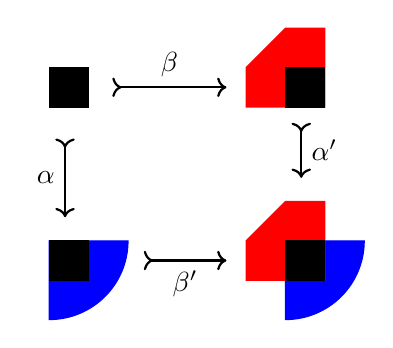
\begin{tikzpicture}  
                \coordinate (k) at (0, 0);
                \draw[black,fill=black] ($(k)+(0,0)$) rectangle ($(k)+(0.5,0.5)$);
                % \node () at ($(k)+(0.25,0.25)$) {\( \mathrm{K} \)};
            
                \coordinate (c) at (0, -2.2);
                \draw[fill=blue,blue]
                ($(c)+(0,-0.5)$)
                -- ($(c)+(0,0.5)$) 
                -- ($(c)+(1,0.5)$) 
                arc[start angle=0, end angle=-90, radius=1]
                -- cycle;
                % \node () at ($(c)+(0.75,0.25)$) {\( \mathrm{C'} \)};
                \draw[black,fill=black] ($(c)+(0,0)$) rectangle ($(c)+(0.5,0.5)$);
                % \node () at ($(c)+(0.25,0.25)$) {\( \mathrm{K} \)};
        
                \coordinate (r) at (3,0);
                \draw[fill=red,red] ($(r)+(-0.5,0)$)
                -- ($(r)+(-0.5,0.5)$)
                -- ($(r)+(0,1)$)
                --  ($(r)+(0.5,1)$)
                -- ($(r)+(0.5,0)$)
                -- cycle;
                % \node () at ($(r)+(-0.23,0.25)$) {\( \mathrm{R'} \)};
                \draw[black,fill=black] ($(r)+(0,0)$) rectangle ($(r)+(0.5,0.5)$);
                % \node () at ($(r)+(0.25,0.25)$) {\( \mathrm{K} \)};
            
                \coordinate (h) at (3, -2.2);
                \draw[fill=blue,blue]
                ($(h)+(0,-0.5)$)
                -- ($(h)+(0,0.5)$)
                -- ($(h)+(1,0.5)$) 
                arc[start angle=0, end angle=-90, radius=1]
                -- cycle;
                \draw[fill=red,red] ($(h)+(-0.5,0)$)
                -- ($(h)+(-0.5,0.5)$)
                -- ($(h)+(0,1)$)
                --  ($(h)+(0.5,1)$)
                -- ($(h)+(0.5,0)$)
                -- cycle;
            % \node () at ($(h)+(0.75,0.25)$) {\( \mathrm{C'} \)};
            \draw[black,fill=black] ($(h)+(0,0)$) rectangle ($(h)+(0.5,0.5)$);
            % \node () at ($(h)+(0.25,0.25)$) {\( \mathrm{K} \)};
            % \node () at ($(h)+(-0.23,0.25)$) {\( \mathrm{R'} \)};
            
                \draw[thick, >->] ($(k)!0.5!(r)+(-0.7,0.25)$)
                        -- node[midway,above] {$\beta$}  
                    ($(k)!0.5!(r)+(0.75,0.25)$);
                % \node (kr) at ($(k)!0.5!(r)+(0.25,0.25)$)
                % {\( \overset{\rightarrowtail}{s} \)};
                % ;  
                \draw[thick, >->]($(c)!0.5!(h)+(-0.3,0.25)$)
                        -- node[midway,below]  {$\beta'$}  
                    ($(c)!0.5!(h)+(0.75,0.25)$);
                
                    \draw[thick, <-<]($(k)!0.5!(c)+(0.2,-0.3)$)
                        -- node[midway,left]  {$\alpha$}  
                    ($(k)!0.5!(c)+(0.2,0.7)$);
                
                    \draw[thick, >->]($(r)!0.5!(h)+(0.2,0.9)$)
                        -- node[midway,right]  {$\alpha'$}  
                    ($(r)!0.5!(h)+(0.2,0.2)$);
            \end{tikzpicture}
        }
        \end{center}
%                 }
%         % }
%     \end{onlyenv}
%     \end{overlayarea}
% \end{minipage}
% \hspace{0.25\textwidth}% small gap
% \begin{minipage}[t]{0.38\textwidth}
%   \begin{overlayarea}{0.4\textwidth}{0.6\textheight}
%     \begin{onlyenv}<5->
%         \resizebox{!}{2\textwidth}{
%                 % \rotatebox{-45}{
    \begin{center}
        \resizebox{0.5\textwidth}{!}{
             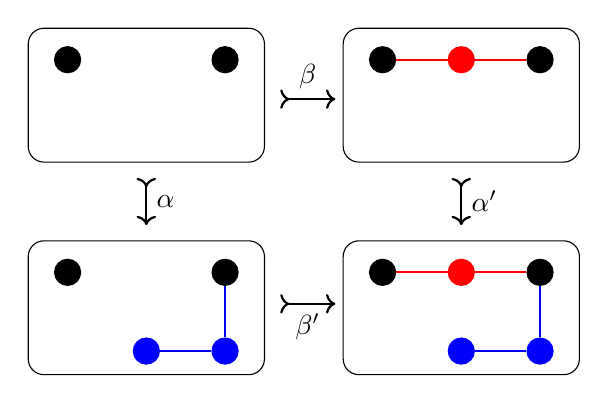
\begin{tikzpicture}
              \graphbox{}{0mm}{5mm}{30mm}{17mm}{2mm}{-5mm}{
                 \coordinate (o) at (-2mm,1mm); 
                  \node[black,fill=black,draw,circle] (l1) at ($(o)+(-10mm,0mm)$) {};
                  \node[black,fill=black,draw,circle] (l2) at ($(l1)+(2,0)$) {};
              } 

              \graphbox{}{40mm}{5mm}{30mm}{17mm}{2mm}{-5mm}{
                \coordinate (o) at (-2mm,1mm); 
                  \node[black,fill=black,draw,circle] (l1) at ($(o)+(-10mm,0mm)$) {};
                  \node[black,fill=black,draw,circle] (l2) at ($(l1)+(2,0)$) {};
                  \node[red,draw,circle,fill=red] (l3) at ($(l1)+(1,0)$) {};
                  \draw[thick, red] (l1) -- (l3) node[midway,above] {};
                  \draw[thick, red] (l3) -- (l2) node[midway,above] {};
              }  

              \graphbox{}{0mm}{-22mm}{30mm}{17mm}{2mm}{-5mm}{
                \coordinate (o) at (-2mm,1mm);
                  \node[black,fill=black,draw,circle] (l1) at ($(o)+(-10mm,0mm)$) {};
                  \node[black,fill=black,draw,circle] (l2) at ($(l1)+(2,0)$) {};
                  \node[blue,draw,circle,fill=blue] (l4) at ($(l2)+(0,-1)$) {};
                  \draw[thick, blue] (l2) -- (l4) node[midway,right] {};
                %   \node[blue,draw,circle] (l6) at ($(l1)+(0,-1)$) {7};
                %   \draw[blue,<-] (l1) -- (l6) node[midway,left] {$a$};
                    \node[blue,draw,circle,fill=blue] (l7) at ($(l4)+(-1,0)$) {};
                  \draw[thick, blue] (l4) -- (l7) node[midway,below] {};
              }    

              \graphbox{}{40mm}{-22mm}{30mm}{17mm}{2mm}{-5mm}{
                \coordinate (o) at (-2mm,1mm);
                  \node[black,fill=black,draw,circle] (l1) at ($(o)+(-10mm,0mm)$) {};
                  \node[black,fill=black,draw,circle] (l2) at ($(l1)+(2,0)$) {};
                  \node[red,draw,circle,fill=red] (l3) at ($(l1)+(1,0)$) {};
                  \node[blue,draw,circle,fill=blue] (l4) at ($(l2)+(0,-1)$) {};
                  \draw[thick, red] (l1) -- (l3) node[midway,above] {};
                  \draw[thick, red] (l3) -- (l2) node[midway,above] {};
                  \draw[thick, blue] (l2) -- (l4) node[midway,right] {};
                %   \node[blue,draw,circle] (l6) at ($(l1)+(0,-1)$) {7};
                %   \draw[blue,<-] (l1) -- (l6) node[midway,left] {$a$};
                \node[blue,draw,circle,fill=blue] (l7) at ($(l4)+(-1,0)$) {};
                  \draw[thick, blue] (l4) -- (l7) node[midway,below] {};
              }    

              % \node () at (37mm,-8mm) {\( \underset{\rightarrowtail}{\beta} \)}; % K -> L
              \draw[thick, >->] (32mm,-4mm) to node[midway,above] {$\beta$} (39mm,-4mm);
              % \node () at (17mm,-18mm) {\(\alpha\ \downarrowtail  \)};
              \draw[thick, >->] (15mm,-14mm) to node[midway,right] {$\alpha$} (15mm,-20mm);
              % \node () at (37mm,-33mm) {\( \overset{\rightarrowtail}{\beta'} \)};
              \draw[thick, >->] (32mm,-30mm) to node[midway,below] {$\beta'$} (39mm,-30mm);
              % \node () at (52mm,-18mm) {\( \downarrowtail\ \alpha' \)};
              \draw[thick, >->] (55mm,-14mm) to node[midway,right] {$\alpha'$} (55mm,-20mm);
      \end{tikzpicture}
        }
    \end{center}
\note{
    si $\alpha$ et $\beta$ sont injectives, on peut voir les graphes en haut a doit et en bas a gauche comme des extensions du graphe en haut a gauche. 
    Et le pushout graphe en bas a droite est obtenu en collant ensemble ces deux extensions le long du graphe commun. 
    Un example concret est montré en bas.

    40s
}
\end{frame}

\section{Graph Rewriting with Double-Pushout (DPO)}

\begin{frame}{Graph Rewriting with Double-Pushout (DPO)}
    \begin{description}
        \item[The first algebraic approach to graph rewriting~\cite{ehrig1973graph}]
        \item[One of the most studied approaches to graph rewriting~\cite{ehrig2006fundamentals}]  
    \end{description}
    \note{
        La réécriture de graphes avec la double poussée est la première approche algébrique des transformations de graphes.
        C'est aussi l'une des approches les plus étudiées des transformations de graphes.

        30s
    }
\end{frame}

\begin{frame}{Graph Rewriting with Double-Pushout (DPO)~\cite{ehrig1973graph}}
    \begin{overlayarea}{\textwidth}{\textheight}
    \begin{beamercolorbox}[rounded=true,shadow=true,wd=\textwidth]{block body}
        \resizebox{!}{0.25\textheight}{
            \begin{tikzpicture}
                \begin{onlyenv}<1->
                    \node (I) at (0,0) {$K$};
                    \node (L) at (-2,0) {$L$};
                    \node (R) at (2,0) {$R$};
                    \draw [thick, ->] (I) to  node [midway,above] {$l$} (L);
                    \draw [thick, ->] (I) to  node [midway,above] {$r$} (R);
                    \draw[fill=red,opacity=0.1 , rounded corners, dotted] (-2.5,-0.5) rectangle (2.5,0.5);
                    \node () at (5.5,0) {Rewriting rule with \textcolor{red}{interface $K$}};
                \end{onlyenv} 
                \begin{onlyenv}<2->
                    \node (G) at (-2,-1.5) {$G$};
                    \draw [thick, >->] (L) to node [midway,right] {} (G);
                \end{onlyenv}
                \begin{onlyenv}<3->
                    \node (C) at (0,-1.5) {$C$};
                    \draw [thick, ->] (I) to node [midway,right] { } (C);
                    \node [at=($(I)!.5!(G)$)] {\normalfont PO};
                    \draw [thick, ->] (C) to node [midway,above] { } (G);
                \end{onlyenv}
                \begin{onlyenv}<4->
                    \node (H) at (2,-1.5) {$H$};
                    \draw [thick, ->] (R) to node [midway,left] { } (H);
                    \draw [thick, ->] (C) to node [midway,above] { } (H);
                    \node [at=($(I)!.5!(H)$)] {\normalfont PO};
                    \draw[fill=PineGreen,opacity=0.1 , rounded corners, dotted] (-2.5,-2) rectangle (2.5,-1);
                    \node () at (5.5,-1.5) {\text{rewriting step $G \Rightarrow H$}};
                \end{onlyenv}
                \end{tikzpicture}
        }
    \end{beamercolorbox}
    \vspace{-0.07\textheight}
  \begin{center}
    \resizebox{\textwidth}{!}{
      \begin{tikzpicture}
            \begin{onlyenv}<1->
                 \graphbox{\( L \)}{0mm}{5mm}{34mm}{15mm}{2mm}{0mm}{
                  \coordinate (o) at (0mm,-8mm); 
                  \node[draw,circle] (l1) at ($(o)+(-10mm,0mm)$) {1};
                  \node[draw,circle] (l2) at ($(l1)+(2,0)$) {2};
                  \node[orange,draw,circle] (l3) at ($(l1)+(1,0)$) {3};
                  \draw[thick, orange,->] (l1) -- (l3) node[midway,above] {$a$};
                  \draw[thick, orange,->] (l3) -- (l2) node[midway,above] {$a$};
              } 

              \graphbox{\( K \)}{40mm}{5mm}{34mm}{15mm}{2mm}{0mm}{
                  \coordinate (o) at (0mm,-8mm); 
                  \node[thick, draw,circle] (l1) at ($(o)+(-10mm,0mm)$) {1};
                  \node[thick, draw,circle] (l2) at ($(l1)+(2,0)$) {2};
              }  

              \graphbox{\( R\)}{80mm}{5mm}{45mm}{15mm}{2mm}{0mm}{
                  \coordinate (o) at (-5mm,-8mm); 
                  \node[draw,circle] (l1) at ($(o)+(-10mm,0mm)$) {1};
                  \node[draw,circle] (l2) at ($(l1)+(3,0)$) {2};
                  \node[red,draw,circle] (l3) at ($(l1)+(1,0)$) {4};
                  \node[red,draw,circle] (l4) at ($(l1)+(2,0)$) {5};
                  \draw[thick, red,->] (l1) -- (l3) node[midway,above] {$a$};
                  \draw[thick, red,->] (l3) -- (l4) node[midway,above] {$b$};
                  \draw[thick, red,->] (l4) -- (l2) node[midway,above] {$a$};
              }    
              \node () at (37mm,-3mm) {\( \overset{l}{\leftarrow} \)}; 
              \node () at (77mm,-3mm) {\( \overset{r}{\rightarrow} \)}; 
            \end{onlyenv} 
            \begin{onlyenv}<2->
                \graphbox{\( G  \)}{0mm}{-17mm}{34mm}{25mm}{2mm}{-5mm}{
                  \coordinate (o) at (0mm,-3mm); 
                  \node[draw,circle] (l1) at ($(o)+(-10mm,0mm)$) {1};
                  \node[draw,circle] (l2) at ($(l1)+(2,0)$) {2};
                  \node[draw,circle,orange] (l3) at ($(l1)+(1,0)$) {3};
                  \node[blue, draw,circle] (l4) at ($(l2)+(0,-1)$) {6};
                  \draw[thick, orange,->] (l1) -- (l3) node[midway,above] {$a$};
                  \draw[thick, orange,->] (l3) -- (l2) node[midway,above] {$a$};
                  \draw[thick, blue,->] (l2) -- (l4) node[midway,right] {$a$};
              }   
              \node () at (17mm,-13mm) {\( \downarrowtail \)};
            \end{onlyenv}
            \begin{onlyenv}<3-> 
                \graphbox{\( C  \)}{40mm}{-17mm}{34mm}{25mm}{2mm}{-5mm}{
                  \coordinate (o) at (0mm,-3mm); 
                  \node[draw,circle] (l1) at ($(o)+(-10mm,0mm)$) {1};
                  \node[draw,circle] (l2) at ($(l1)+(2,0)$) {2};
                  \node[blue,draw,circle] (l4) at ($(l2)+(0,-1)$) {6};
                  \draw[thick, blue,->] (l2) -- (l4) node[midway,right] {$a$};
                 }   
                \node () at (37mm,-28mm) {\( \leftarrow \)};
                 \node () at (52mm,-13mm) {\( \downarrow \)};
                 \node () at (37mm,-15mm) {\text{PO}};
            \end{onlyenv}
            \begin{onlyenv}<4-> 
              \graphbox{\( H   \)}{80mm}{-17mm}{45mm}{25mm}{2mm}{-5mm}{
                  \coordinate (o) at (-5mm,-3mm); 
                  \node[draw,circle] (l1) at ($(o)+(-10mm,0mm)$) {1};
                  \node[draw,circle] (l2) at ($(l1)+(3,0)$) {2};
                  \node[draw,circle,red] (l3) at ($(l1)+(1,0)$) {4};
                  \node[draw,circle,red] (l4) at ($(l1)+(2,0)$) {5};
                  \node[blue,draw,circle] (l5) at ($(l2)+(0,-1)$) {6};
                  \draw[thick, red,->] (l1) -- (l3) node[midway,above] {$a$};
                  \draw[thick, red,->] (l3) -- (l4) node[midway,above] {$b$};
                  \draw[thick, red,->] (l4) -- (l2) node[midway,above] {$a$};
                  \draw[thick, blue,->] (l2) -- (l5) node[midway,right] {$a$};
              }    
              \node () at (92mm,-13mm) {\( \downarrow \)};
              \node () at (77mm,-28mm) {\( \rightarrow \)}; 
                 \node () at (77mm,-15mm) {\text{PO}};
            \end{onlyenv} 
            
      \end{tikzpicture}
      }
   \end{center}
\end{overlayarea}
\note{
    Une regle de réécriture de graphes avec double pushout est un couple de morphismes l et r qui partent le meme graphe de depart K, appelé l'interface.

    Pour appliquer cette regle a un graphe G, on cherche un morphisme injectif de L vers G, appelé le match.

    Ensuite, on construit un diagram de pushout. 

    Le graphe C est obtenu en supprimant de G les elements qui sont dans L mais pas dans K. 

    Finalement, on construit un autre diagram de pushout.

    Une etape de réécriture de graphes est ainsi obtenue, transformant G en H.

    70s
}
\end{frame}

\begin{frame}{An Invalid Rewriting Step}
    % of the edge \textcolor{red}{$3 \overset{a}{\rightarrow} 6$} in $G$:
    \begin{center}
        \resizebox{\textwidth}{!}{
        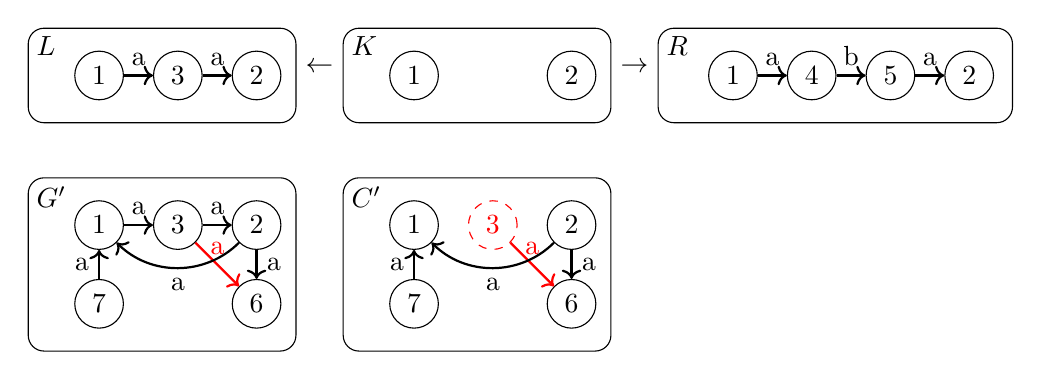
\begin{tikzpicture}
            \graphbox{\( L \)}{0mm}{-3mm}{34mm}{12mm}{2mm}{2mm}{
                \coordinate (o) at (0mm,-8mm); 
                \node[draw,circle] (l1) at ($(o)+(-10mm,0mm)$) {1};
                \node[draw,circle] (l2) at ($(l1)+(2,0)$) {2};
                \node[draw,circle] (l3) at ($(l1) + (1,0)$) {3};
                \draw[thick, ->] (l1) -- (l3) node[midway,above] {a};
                \draw[thick, ->] (l3) -- (l2) node[midway,above] {a};
            } 
    
            \graphbox{\( K \)}{40mm}{-3mm}{34mm}{12mm}{2mm}{2mm}{
                \coordinate (o) at (0mm,-8mm); 
                \node[draw,circle] (l1) at ($(o)+(-10mm,0mm)$) {1};
                \node[draw,circle] (l2) at ($(l1)+(2,0)$) {2};
            }  
    
            \graphbox{\( R \)}{80mm}{-3mm}{45mm}{12mm}{2mm}{2mm}{
                \coordinate (o) at (-5mm,-8mm); 
                \node[draw,circle] (l1) at ($(o)+(-10mm,0mm)$) {1};
                \node[draw,circle] (l2) at ($(l1)+(3,0)$) {2};
                \node[draw,circle] (l3) at ($(l1) + (1,0)$) {4};
                \node[draw,circle] (l4) at ($(l1) + (2,0)$) {5};
                \draw[thick, ->] (l1) -- (l3) node[midway,above] {a};
                \draw[thick, ->] (l3) -- (l4) node[midway,above] {b};
                \draw[thick, ->] (l4) -- (l2) node[midway,above] {a};
            }    
    
            \graphbox{\( G' \)}{0mm}{-22mm}{34mm}{22mm}{2mm}{-3mm}{
                \coordinate (o) at (0mm,-3mm); 
                \node[draw,circle] (l1) at ($(o)+(-10mm,0mm)$) {1};
                \node[draw,circle] (l2) at ($(l1)+(2,0)$) {2};
                \node[draw,circle] (l3) at ($(l1) + (1,0)$) {3};
                \node[draw,circle] (l4) at ($(l2) + (0,-1)$) {6};
                \draw[thick, ->,red] (l3) -- (l4) node[midway,above] {a};
                \draw[thick, ->] (l1) -- (l3) node[midway,above] {a};
                \draw[thick, ->] (l3) -- (l2) node[midway,above] {a};
                \draw[thick, ->] (l2) -- (l4) node[midway,right] {a};
                \node[draw,circle] (l6) at ($(l1) + (0,-1)$) {7};
                \draw[thick, <-] (l1) -- (l6) node[midway,left] {a};
                \draw[thick, ->] (l2) edge[out=-135,in=-45]node[midway,below] {a} (l1) ;
            }    
            % \onslide<2->{
                \graphbox{\( C'  \)}{40mm}{-22mm}{34mm}{22mm}{2mm}{-3mm}{
                    \coordinate (o) at (0mm,-3mm); 
                    \node[draw,circle] (l1) at ($(o)+(-10mm,0mm)$) {1};
                    \node[draw,circle] (l2) at ($(l1)+(2,0)$) {2};
                    \node[draw,circle] (l4) at ($(l2) + (0,-1)$) {6};
                    \node[draw,circle,dashed,red] (l3) at ($(l1) + (1,0)$) {3};
                    % \draw[->,red] (l3) -- (l4) node[midway,above] {a};
                    \draw[thick, ->,red] (l3) -- (l4) node[midway,above] {a};
                    \draw[thick, ->] (l2) -- (l4) node[midway,right] {a};
                    \draw[thick, ->] (l2) edge[out=-135,in=-45]node[midway,below] {a} (l1) ;
                    \node[draw,circle] (l6) at ($(l1) + (0,-1)$) {7};
                    \draw[thick, <-] (l1) -- (l6) node[midway,left] {a};
                }    
    
            % \graphbox{\( H' \)}{80mm}{-22mm}{45mm}{22mm}{2mm}{-3mm}{
            %     \coordinate (o) at (-5mm,-3mm); 
            %     \node[draw,circle] (l1) at ($(o)+(-10mm,0mm)$) {1};
            %     \node[draw,circle] (l2) at ($(l1)+(3,0)$) {2};
            %     \node[draw,circle] (l3) at ($(l1) + (1,0)$) {4};
            %     \node[draw,circle] (l4) at ($(l1) + (2,0)$) {5};
            %     \node[draw,circle] (l5) at ($(l2) + (0,-1)$) {6};
            %     \node[draw,circle] (l6) at ($(l1) + (0,-1)$) {7};
            %     \draw[<-] (l1) -- (l6) node[midway,left] {a};
            %     \draw[->] (l1) -- (l3) node[midway,above] {a};
            %     \draw[->] (l3) -- (l4) node[midway,above] {b};
            %     \draw[->] (l4) -- (l2) node[midway,above] {a};
            %     \draw[->] (l2) -- (l5) node[midway,right] {a};
            %     \draw[->] (l2) edge[out=-135,in=-45]node[midway,below] {a} (l1) ;
            %     \node[draw,circle,dashed,red] (l3) at (-0mm,-7mm) {3};
            %     \draw[->,red] (l3) -- (l5) node[midway,above] {a};
            % }    
    
            \node () at (37mm,-8mm) {\( \leftarrow \)}; % K -> L
            \node () at (77mm,-8mm) {\( \rightarrow \)}; % K -> R
            \node () at (15mm,-18mm) {\(\downarrowtail \)};
            % \node () at (37mm,-33mm) {\( \leftarrow \)};
            % \node () at (37mm,-18mm) {PO};
            % \node () at (58mm,-18mm) {\( \downarrow \)}; 
            % \node () at (80mm,-18mm) {PO};
            % \node () at (102mm,-18mm) {\( \downarrow \)};
            % \node () at (77mm,-33mm) {\( \rightarrow \)}; % C -> H
        \end{tikzpicture}
        }         
    \end{center}
    \note{
        Voici un exemple d'une etape de réécriture qui n'est pas valide.

        En effet, la suppression du noeud 3 cree une arete dans la vide.

        20s

        % 20s 70s 30s 40s 1m 45s 45s = 5m10s
    } 
\end{frame}

\section{Toward Greater Usability}
% \begin{frame}
%   \tableofcontents[currentsection, hideothersubsections]
% \end{frame}

\begin{frame}{Weighted Type Graph Method~\cite{bruggink2014termination,bruggink2015proving,endrullis2024generalized_icgt}}
Termination by interpretation
\newline\newline
Parameter: an object $T$ in the category, called \textcolor{PineGreen}{type graph}
\newline\newline
Terminology: every graph is \enquote{typed} as morphisms to $T$
\newline\newline
Interpretation:
\vspace{-3mm}
\begin{flalign*}
G &\leadsto \mathrm{morphisms}(G,T) \\
  &\leadsto \mathrm{weight}(\mathrm{morphisms}(G,T)) \\
  &\leadsto \mathrm{aggregator}(\mathrm{weight}(\mathrm{morphisms}(G,T)))\in\mathbb{N}
\end{flalign*}

% \only<2->{
\alert{
How to choose the type graph $T$?
\newline
What is the morphism weight?
\newline
What is the graph weight?}
\note{
    La méthode par graphe de type pondéré est une méthode de terminaison par interprétation.

    Cette methode a un paramètre qui est un objet T, appelé graphe de type.

    Son nom vient du fait que chaque graphe $G$ est consideré comme étant typé par l'ensemble des morphismes de $G$ vers $T$.

    Un graphe $G$ est tout d'abord interprété comme l'ensemble des morphismes de $G$ vers $T$.
    Ensuite, chaque morphisme est interprété comme un entier naturel.
    Finalement, les poids des morphismes sont agrégés pour obtenir un entier naturel.

    La question est alors comment choisir le graphe de type T, comment définir le poids d'un morphisme, et comment agréger les poids des morphismes.

    Il y a 3 configurations possibles, on va utiliser un example dans une configuration pour donner une intuition.
    
    90s
}
\end{frame}

\begin{frame}{Type Graph with Weights on Edges}
    \phantom{
        \begin{beamercolorbox}[rounded=true,shadow=true,wd=\textwidth]{block body}
        The weight of a morphism $h: G \rightarrow T$ is \[\sum_{e \in \opn{Edge(G)}}\mathrm{weight}(h(e)) \]
        \end{beamercolorbox}
    }
     \begin{center}
        \resizebox{\textwidth}{!}{
            \begin{tikzpicture}
              \phantom{
                \graphbox{\(L\)}{2mm}{0mm}{30mm}{20mm}{0mm}{0mm}{
                        \coordinate (o) at (0mm,-10mm); 
                        \node[draw,circle] (l1) at ($(o)+(-10mm,0mm)$) {};
                        \node[draw,circle] (l2) at ($(l1)+(2,0)$) {};
                        \node[draw,circle] (l3) at ($(l1)+(1,0)$) {};
                        \draw[->,red] (l1) -- (l3) node[midway,above] {$a$};
                        \draw[->,PineGreen] (l3) -- (l2) node[midway,above] {$b$};
                    } 
                  \graphbox{$T$}{-42mm}{10mm}{33mm}{40mm}{-8mm}{-20mm}{
                    \node[draw,circle] (1) at (0,0) {};
                    \node[draw,circle] (2) at (2,0) {};
                    \draw[->,red] (1) edge[loop above] node[midway, above] {$a^{1}$} (1) ;
                    \draw[->,PineGreen] (1) edge[loop below] node[midway, below] {$b^{0}$} (1) ;
                    \draw[->] (1) edge[bend left] node[midway, above] {$a^{0}$}  (2)  ;
                    \draw[->] (2) edge[bend left] node[midway, below] {$b^{0}$} (1) ;
                  }
                % \node () at (-3mm,-10mm) {$\overset{h_1}{\leftarrow}$};
                \draw[<-] (-7mm,-10mm) to node[midway,above] {$h_1$} (0mm,-10mm);
                 % \node () at (43mm,-10mm) {$\overset{h_2}{\to}$};
                    \draw[->] (34mm,-10mm) to node[midway,above] {$h_2$} (43mm,-10mm);
              }
            
                \graphbox{$T$}{45mm}{10mm}{35mm}{40mm}{-10mm}{-19mm}{
                    \node[draw,circle] (1) at (0,0) {};
                    \node[draw,circle] (2) at (2,0) {};
                    \draw[->] (1) edge[loop above] node[midway, above] {$a^{1}$} (1) ;
                    \draw[->] (1) edge[loop below] node[midway, below] {$b^{0}$} (1) ;
                    \draw[->,red] (1) edge[bend left] node[midway, above] {$a^{0}$}  (2)  ;
                    \draw[->,PineGreen] (2) edge[bend left] node[midway, below] {$b^{0}$} (1);
                }
                  
            \end{tikzpicture}
            }
    \end{center}
    % \begin{center}
    % \resizebox{0.8\textwidth}{!}{
    %      \begin{tikzpicture}
    %        \phantom{
    %       \graphbox{}{-50mm}{0mm}{40mm}{39mm}{2mm}{-6mm}{
    %         \coordinate (o) at (0mm,-10mm); 
    %         \node[draw,circle] (l1) at ($(o)+(-10mm,0mm)$) {};
    %         \node[draw,circle] (l2) at ($(l1)+(2,0)$) {};
    %         \node[draw,circle] (l3) at ($(l1)+(1,0)$) {};
    %         \draw[red,->] (l1) -- (l3) node[midway,above] {$a$};
    %         \draw[PineGreen,->] (l3) -- (l2) node[midway,above] {$b$};
    %     } 
    %     \draw[->] (-9mm,-17mm) to node[midway,above] {$h$} (-2mm,-17mm);
    % }
    %         \graphbox{$T$}{0mm}{0mm}{40mm}{39mm}{-12mm}{-19mm}{
    %             \node[draw,circle] (1) at (0,0) {};
    %             \node[draw,circle] (2) at (2,0) {};
    %             \draw[->] (1) edge[loop above] node[midway, above] {$a^{1}$} (1);
    %             \draw[->] (1) edge[loop below] node[midway, below] {$b^{0}$} (1);
    %             \draw[->,red] (1) edge[bend left] node[midway, above] {$a^{0}$}  (2);
    %             \draw[->,PineGreen] (2) edge[bend left] node[midway, below] {$b^{0}$} (1);
    %         }
    %     \end{tikzpicture}
    %     }
    % \end{center}
    \phantom{
            $ \mathrm{weight}_T(h) \mathop{=} \textcolor{red}{0} + \textcolor{PineGreen}{0} \mathop{=} 0$
        }

    \note{
        Voici un exemple d'un graphe de type avec des poids sur les arêtes.


       10s
    }
\end{frame}
\begin{frame}{Morphism Weight}
     \begin{beamercolorbox}[rounded=true,shadow=true,wd=\textwidth]{block body}
      The weight of a morphism $h: G \rightarrow T$ is \[\sum_{e \in \opn{Edge(G)}}\mathrm{weight}(h(e)) \]
    \end{beamercolorbox}
    \begin{center}
        \resizebox{\textwidth}{!}{
            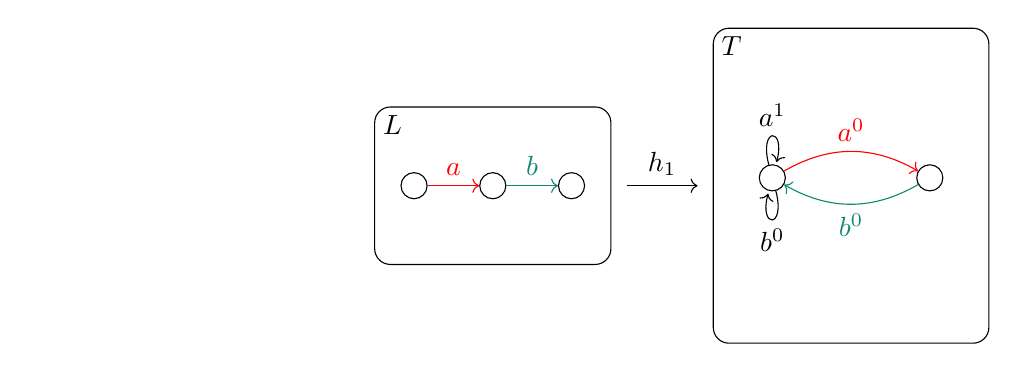
\begin{tikzpicture}
                \graphbox{\(L\)}{2mm}{0mm}{30mm}{20mm}{0mm}{0mm}{
                    \coordinate (o) at (0mm,-10mm); 
                    \node[draw,circle] (l1) at ($(o)+(-10mm,0mm)$) {};
                    \node[draw,circle] (l2) at ($(l1)+(2,0)$) {};
                    \node[draw,circle] (l3) at ($(l1)+(1,0)$) {};
                    \draw[->,red] (l1) -- (l3) node[midway,above] {$a$};
                    \draw[->,PineGreen] (l3) -- (l2) node[midway,above] {$b$};
                } 
              \phantom{
                  \graphbox{$T$}{-42mm}{10mm}{33mm}{40mm}{-8mm}{-20mm}{
                    \node[draw,circle] (1) at (0,0) {};
                    \node[draw,circle] (2) at (2,0) {};
                    \draw[->,red] (1) edge[loop above] node[midway, above] {$a^{1}$} (1) ;
                    \draw[->,PineGreen] (1) edge[loop below] node[midway, below] {$b^{0}$} (1) ;
                    \draw[->] (1) edge[bend left] node[midway, above] {$a^{0}$}  (2)  ;
                    \draw[->] (2) edge[bend left] node[midway, below] {$b^{0}$} (1) ;
                  }
                % \node () at (-3mm,-10mm) {$\overset{h_1}{\leftarrow}$};
                \draw[<-] (-7mm,-10mm) to node[midway,above] {$h_1$} (0mm,-10mm);
              }
            
                \graphbox{$T$}{45mm}{10mm}{35mm}{40mm}{-10mm}{-19mm}{
                    \node[draw,circle] (1) at (0,0) {};
                    \node[draw,circle] (2) at (2,0) {};
                    \draw[->] (1) edge[loop above] node[midway, above] {$a^{1}$} (1) ;
                    \draw[->] (1) edge[loop below] node[midway, below] {$b^{0}$} (1) ;
                    \draw[->,red] (1) edge[bend left] node[midway, above] {$a^{0}$}  (2)  ;
                    \draw[->,PineGreen] (2) edge[bend left] node[midway, below] {$b^{0}$} (1);
                }
                   % \node () at (43mm,-10mm) {$\overset{h_2}{\to}$};
                    \draw[->] (34mm,-10mm) to node[midway,above] {$h_1$} (43mm,-10mm);
            \end{tikzpicture}
            }
    \end{center}
    % \begin{center}
    % \resizebox{0.8\textwidth}{!}{
    %      \begin{tikzpicture}
    %       \graphbox{}{-50mm}{0mm}{40mm}{39mm}{2mm}{-6mm}{
    %         \coordinate (o) at (0mm,-10mm); 
    %         \node[draw,circle] (l1) at ($(o)+(-10mm,0mm)$) {};
    %         \node[draw,circle] (l2) at ($(l1)+(2,0)$) {};
    %         \node[draw,circle] (l3) at ($(l1)+(1,0)$) {};
    %         \draw[red,->] (l1) -- (l3) node[midway,above] {$a$};
    %         \draw[PineGreen,->] (l3) -- (l2) node[midway,above] {$b$};
    %     } 
    %     \draw[->] (-9mm,-17mm) to node[midway,above] {$h$} (-2mm,-17mm);
    %         \graphbox{$T$}{0mm}{0mm}{40mm}{39mm}{-12mm}{-19mm}{
    %             \node[draw,circle] (1) at (0,0) {};
    %             \node[draw,circle] (2) at (2,0) {};
    %             \draw[->] (1) edge[loop above] node[midway, above] {$a^{1}$} (1);
    %             \draw[->] (1) edge[loop below] node[midway, below] {$b^{0}$} (1);
    %             \draw[->,red] (1) edge[bend left] node[midway, above] {$a^{0}$}  (2);
    %             \draw[->,PineGreen] (2) edge[bend left] node[midway, below] {$b^{0}$} (1);
    %         }
    %     \end{tikzpicture}
    %     }
    % \end{center}
            \hspace{0.65\textwidth}$ \mathrm{weight}_T(h_1) \mathop{=} \textcolor{red}{0} + \textcolor{PineGreen}{0} \mathop{=} \textcolor{PineGreen}{0}$
    \note{
        Pour calculer le poids du morphisme h1, on somme les poids des images des arêtes de L.

        10s
    }
\end{frame}
 

\begin{frame}{Graph Weight} 
    \begin{beamercolorbox}[rounded=true,shadow=true,wd=\textwidth]{block body}
        The weight of a graph $L$ is \[\min \{h : L \mathop{\to} T \mid \mathrm{weight}_T(h)\}\]
    \end{beamercolorbox}
    \vspace{0.09\textheight}
    \begin{center}
        \resizebox{\textwidth}{!}{
            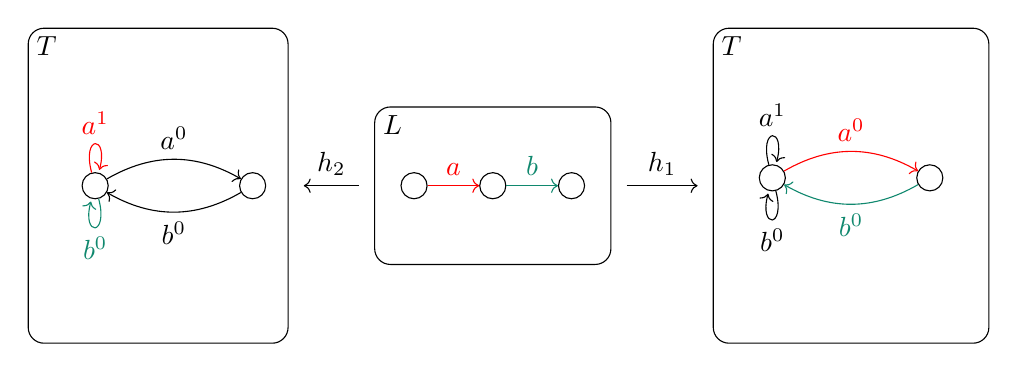
\begin{tikzpicture}
                \graphbox{\(L\)}{2mm}{0mm}{30mm}{20mm}{0mm}{0mm}{
                    \coordinate (o) at (0mm,-10mm); 
                    \node[draw,circle] (l1) at ($(o)+(-10mm,0mm)$) {};
                    \node[draw,circle] (l2) at ($(l1)+(2,0)$) {};
                    \node[draw,circle] (l3) at ($(l1)+(1,0)$) {};
                    \draw[->,red] (l1) -- (l3) node[midway,above] {$a$};
                    \draw[->,PineGreen] (l3) -- (l2) node[midway,above] {$b$};
                } 
                \graphbox{$T$}{-42mm}{10mm}{33mm}{40mm}{-8mm}{-20mm}{
                    \node[draw,circle] (1) at (0,0) {};
                    \node[draw,circle] (2) at (2,0) {};
                    \draw[->,red] (1) edge[loop above] node[midway, above] {$a^{1}$} (1) ;
                    \draw[->,PineGreen] (1) edge[loop below] node[midway, below] {$b^{0}$} (1) ;
                    \draw[->] (1) edge[bend left] node[midway, above] {$a^{0}$}  (2)  ;
                    \draw[->] (2) edge[bend left] node[midway, below] {$b^{0}$} (1) ;
                }
            
                \graphbox{$T$}{45mm}{10mm}{35mm}{40mm}{-10mm}{-19mm}{
                    \node[draw,circle] (1) at (0,0) {};
                    \node[draw,circle] (2) at (2,0) {};
                    \draw[->] (1) edge[loop above] node[midway, above] {$a^{1}$} (1) ;
                    \draw[->] (1) edge[loop below] node[midway, below] {$b^{0}$} (1) ;
                    \draw[->,red] (1) edge[bend left] node[midway, above] {$a^{0}$}  (2)  ;
                    \draw[->,PineGreen] (2) edge[bend left] node[midway, below] {$b^{0}$} (1);
                }
                % \node () at (43mm,-10mm) {$\overset{h_2}{\to}$};
                \draw[->] (34mm,-10mm) to node[midway,above] {$h_1$} (43mm,-10mm);
                % \node () at (-3mm,-10mm) {$\overset{h_1}{\leftarrow}$};
                \draw[<-] (-7mm,-10mm) to node[midway,above] {$h_2$} (0mm,-10mm);
            \end{tikzpicture}
            }
    \end{center}
    \begin{flalign*}
      & \mathrm{weight}_T(h_2) \mathop{=} \textcolor{red}{1} + \textcolor{PineGreen}{0} \mathop{=} \textcolor{red}{1} \hspace{0.1\textwidth} &\mathrm{weight}_T(h_1) \mathop{=} \textcolor{red}{0} + \textcolor{PineGreen}{0} \mathop{=} \textcolor{PineGreen}{0}\\
      &\mathrm{weight}_T(L) \mathop{=} \min \{\textcolor{red}{1}, \textcolor{PineGreen}{0}\} \mathop{=} 0 &
    \end{flalign*}
        % $\mathrm{weight}_T(L) \mathop{=} \min \{,\mathrm{weight}_T(h_2)\} = \min \{1+1, 1+0\}\mathop{=} 1$     
    \note{
        Pour calculer le poids du graphe L, on calcule d'abord les poids de tous les morphismes de L vers T.
        Ensuite, on prend le minimum de ces poids.

        Pour cet exemple, il y a deux morphismes, h1 et h2. 
        Le poids de h1 est 0, et le poids de h2 est 1.
        Donc, le poids de L est 0.

        40s
    }  
\end{frame}
   
\begin{frame}{Termination Criterion~\cite{bruggink2015proving}}
    %   \begin{beamercolorbox}[rounded=true,shadow=true,wd=\textwidth]{block body}
    \begin{center}
    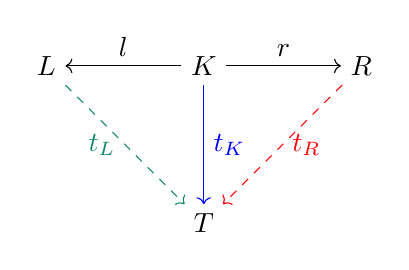
\begin{tikzpicture}
            \node (k) at (0,0) {$K$};
            \node (l) at (-2,0) {$L$};
            \node (t) at (0,-2) {$T$};
            \node (r) at (2,0) {$R$};
            \draw [->] (k) to  node [midway,above] {$l$} (l);
            \draw [->] (k) to  node [midway,above] {$r$} (r);
            \draw [->,blue] (k) to  node [midway,right] {\textcolor{blue}{$t_K$}} (t);
            \draw [->,dashed,PineGreen] (l) to node [midway,left] {\textcolor{PineGreen}{$t_L$}} (t);
            \draw [->,dashed,red] (r) to node [midway,right] {\textcolor{red}{$t_R$}} (t);
        \end{tikzpicture}
    \end{center}

      \begin{beamercolorbox}[rounded=true,shadow=true,wd=\textwidth]{block body}
        % Every rewriting step strictly decreases the weight
        A rule terminates \textcolor{red}{if there is $T$} such that for all \textcolor{blue}{$t_K$}, if there is \textcolor{PineGreen}{$t_L$} such that $\triangle KLT$ commutes, then 
        \begin{flalign*}
            &\min \{\opn{weight}_T(\textcolor{PineGreen}{t_L}) \mid t_L.\triangle KLT \text{commutes}\}  
            \\ \mathop{>}
            &\min \{\opn{weight}_T(\textcolor{red}{t_R}) \mid t_R.\triangle KRT \text{commutes}\}  
        \end{flalign*}
    \end{beamercolorbox}
 
   \alert{How to find a suitable weighted type graph?}
   \note{ 
        Voici le critère de terminaison.

        Une règle de réécriture termine s'il existe un graphe de type T tel que pour tout morphisme tK de K vers T, si il existe un morphisme tL de L vers T tel que le triangle KLT commute, alors le poids minimal des morphismes tL tels que le triangle KLT commute est strictement supérieur au poids minimal des morphismes tR tels que le triangle KRT commute.

        La question est alors comment trouver un graphe de type pondéré approprié.
   }
\end{frame}

\begin{frame}{Searching for Weighted Type Graphs over $\mathbb{N}$~\cite{zantema2014termination,bruggink2015proving}}
    % Restricted search space:
    %   \begin{itemize}
    %     \item no parallel edges of the same label 
    %   \end{itemize}
    User-specified parameters:
      \begin{itemize}
        \item \alert{$k$ nodes}
        \item \alert{maximum edge weight $n\in\mathbb{N}$}
      \end{itemize}   
    The problem amounts to checking the \textcolor{red}{satisfiability of an
existential Presburger arithmetic theory} with:
                \begin{itemize}
                  \item $k^2m$ binary variables where $m$ is the number of labels
                  \item $k^2m$ integer variables
                \end{itemize} 
  Challenge:
  \begin{itemize}
    \item expertise: impossible to guess $k$ and $n$
    \item complexity: $2^{k^2m} \cdot n^{k^2m}$ possible assignments of weights
  \end{itemize} 

  \note{ 
    Les travaux précédents suggerent de se restreindre à des graphes de type avec un nombre fixe de noeuds k et un poids maximum n. 
    Le problème revient à vérifier la satisfiabilité d'une théorie existentielle de l'arithmétique de Presburger avec des variables binaires et des variables entières.
    Le défi est double: d'une part, il est impossible pour l'utilisateur de deviner k et n.
    D'autre part, il y a un nombre exponentiel d'affectations des poids.

    1m
  }
\end{frame}


\begin{frame}{Problem of the Size of the Search Space}
% def f(k, m, n) -> int:
%     e = pow(k,2) * m
%     left = pow(2,e)
%     right = pow(n,e)
%     return left * right
With natural numbers as weights:
    \begin{center}
    \begin{tabular}{ |c|c|c|c| } 
    \hline
    \# nodes (k)&  \# labels (m) & \# weights & \# possibilities \\ 
    \hline
    2 & 2 & 2 & $\approx 10^{4}$ \\ 
    \hline
    3 & 3 & 3 & $\approx  10^{21}$ \\ 
    % \hline
    % 3 & 3 & 10 & $\approx   10^{45}$ \\
    % \hline
    % 3 & 3 & 100 & $\approx 10^{87}$ \\
    \hline
    4 & 4 & 4 & $\approx  10^{57}$ \\ 
    \hline
    % 4 & 4 & 10 & $\approx 10^{95}$ \\
    %  \hline
    % 4 & 4 & 100 & $\approx 10^{181}$ \\
    5 & 5 & 5 & $\approx 10^{125}$ \\
    \hline
    \end{tabular}
    \end{center}

    Problems can solved by Z3 in exponential-time with respect to the number of variables $2k^2m$.

    \note{
        Voici quelques exemples du nombre d'affectations des poids en fonction des nombres de noeuds, d'étiquettes, et de poids.

        On peut voir que le nombre de possibilités croît très rapidement.

        Z3 peut résoudre les problèmes en temps exponentiel par rapport au nombre de variables.

        30s        
    }

\end{frame}
\begin{frame}{Usability Improvement}
    Using positive real numbers as weights~\cite{lucas2006relative}

    \vspace{0.5cm}
    Additional constraint: there is \textcolor{red}{$\delta > 0$} such that every rewriting step decreases the weight by at least \textcolor{red}{$\delta$}.
 
    \note{ 
        Afin d'améliorer l'utilisabilité de la méthode, on propose d'utiliser des nombres réels positifs comme poids.
        
        Une contrainte supplementaire est tout fois nécessaire: il doit exister un delta strictement positif tel que chaque étape de réécriture diminue le poids d'au moins delta.

        30s
    }
\end{frame}

% \begin{frame}{Searching for Weighted Type Graphs over \crossout[red]{$\mathbb{N}$} $\mathbb{R}$}
%     User-specified parameters:
%       \begin{itemize}
%         \item \alert{$k$ nodes}
%         \item \crossout[red]{edge weights in $\{0, 1, \ldots, n\}$}
%       \end{itemize}   
%     % Assumption:
%     %   \begin{itemize}
%     %     \item no parallel edges of the same label 
%     %   \end{itemize}
%     The problem amounts to checking the satisfiability of an
% \crossout[red]{existential Presburger arithmetic theory} \textcolor{red}{existential theory of the reals with binary variables}:
%                 \begin{itemize}
%                   \item $k^2m$ binary variables where $m$ is the number of labels
%                   \item $k^2m$ \crossout[red]{integer} \textcolor{red}{real} variables
%                 \end{itemize} 
% %   Challenge:
% %   \begin{itemize}
% %     \item \crossout[red]{there are $2^{k^2m} \cdot n^{k^2m}$ possible assignments of weights}. \textcolor{red}{There are $2^{k^2m}$ linear programs which have polynomial-time average-case complexity.}
% %   \end{itemize} 
%     Challenge:
%   \begin{itemize}
%     \item impossible to guess $k$ and \crossout[red]{maximum weight $n$}
%     \item complexity: \crossout[red]{$2^{k^2m} \cdot n^{k^2m}$ possible assignments of weights} \textcolor{red}{there are $2^{k^2m}$ linear programs with $k^2m$ real variables, which have polynomial-time average-case complexity.}
%   \end{itemize} 
%     \note{ 
%         L'utilisateur n'a plus besoin de deviner le poids maximum.

%         Le problème revient à vérifier la satisfiabilité d'une théorie existentielle des réels avec des variables binaires et des variables réelles.

%         Il suffit de résoudre un nombre relativement petit de programmes linéaires avec peu de variables réelles. Ces programmes linéaires peuvent être résolus en temps polynomial en moyenne par rapport au nombre de variables par un solver.

%         1m
%     }
% \end{frame}


\begin{frame}{Complexity Comparison}
% def f(k, m, n) -> int:
%     e = pow(k,2) * m
%     left = pow(2,e)
%     right = pow(n,e)
%     return left * right
$m$: number of labels

Parameters:
\begin{itemize}
    \item $k$ nodes
\end{itemize}

With weights in $\mathbb{N}$:
\begin{itemize}
    \item \textcolor{red}{User-specified} parameter: maximum weight $n\in\mathbb{N}$
    \item \textcolor{red}{Satisfiability of an
existential Presburger arithmetic theory} with $k^2m$ variables
    \item \textcolor{PineGreen}{Exponential-time}
\end{itemize}
With weights in $\mathbb{R}$:
    \begin{itemize}
        \item \textcolor{red}{Solve a linear program in $\mathbb{R}$ with $k^2m$ variables}
        \item \textcolor{PineGreen}{Polynomial time on average} (e.g by Z3)
    \end{itemize} 
\note{
    Voici une comparaison de la complexité entre les deux approches pour un nombre de noeuds k fixe.

    Avec des poids dans les entiers naturels, l'utilisateur doit deviner un poids maximum n.
    Ensuite, il faut vérifier la satisfiabilité d'une théorie existentielle de l'arithmétique de Presburger avec k^2m variables entières.
    Cette vérification demande un temps exponentiel au moins par rapport au nombre de variables.

    Avec des poids dans les réels, 
    on n'a plus besoin de deviner un poids maximum, 
    et il suffit de résoudre un programme linéaire dans les réels.
    La résolution de ce programme linéaire peut être faite en temps polynomial en moyenne par un solver comme Z3.

    75s
}
\end{frame}

\begin{frame}{Experimental Results}
 
    \begin{table}[htb]   
        \renewcommand{\arraystretch}{1.2}
        \centering
        \begin{adjustbox}{max width=\textwidth,max totalheight=0.8\textheight,keepaspectratio}
    \begin{tabular}{|c|c|c|c|c|c|c |}
        \hline
        &\;\;$A_{\mathbb{N}}$\;\;&\;\;$a_{\textcolor{red}{\mathbb{R}}}$\;\;&\;\;$T_{\mathbb{N}}$\;\;&\;\;$t_{\textcolor{red}{\mathbb{R}}}$\;\;&\;\; $N_{\mathbb{N}}$\;\;&\;\;$n_{\textcolor{red}{\textcolor{red}{\mathbb{R}}}}$\;\; \\
        \hline
    % ~\cite[Example 6.2]{endrullis2024generalized_arxiv_v2} & & & & & 2.68 &1.15   \\
    ~\cite[Example 6.3]{endrullis2024generalized_arxiv_v2} & & & & & 2.74 &\textcolor{PineGreen}{1.16}   \\
        %~\cite[Example 6.4]{endrullis2024generalized_arxiv_v2}&  && & &  &   &  &  & our only Graph\\
    ~\cite[Example D.3]{endrullis2024generalized_arxiv_v2} &2.25 
        % (2.30+2.188+2.2637+2.2928+ 2.196) 
        & \textcolor{PineGreen}{1.18}
        % (1.17+1.2549+1.165+ 1.1576\mathop{+}1.162)
        & & & 2.24& \textcolor{PineGreen}{1.18}    \\
    ~\cite[Example 3.8]{plump1995ontermination}
    & 2.95& \textcolor{PineGreen}{1.90} & 2.94 &\textcolor{PineGreen}{1.87}  & 3.49  &\textcolor{PineGreen}{1.87}   \\
        %~\cite[Example 3]{plump2018modular}
        % & 3.45& 3.44 & 3.55 &2.38  & 3.96  &17.60 &   4.24 AT &  3.45 at& 4.07 t  \\
    ~\cite[Example 4]{plump2018modular} &4.26& \textcolor{PineGreen}{3.19} &  4.24 & \textcolor{PineGreen}{3.13} &
        5.82
        % (5.77+5.83+5.775+5.84+5.818+5.89)
        & \textcolor{red}{timeout}  \\

    ~\cite[Example 5]{plump2018modular} & 5.54
        &\textcolor{red}{5.55}
        % (5.53 +5.660\mathop{+}5.5213+5.5369+5.484689\mathop{+}5.6404\mathop{+}5.4877\mathop{+}5.5026)
        & 5.53& \textcolor{PineGreen}{5.50}& 9.11&  \textcolor{PineGreen}{5.62}  \\
    % ~\cite[Example 6]{plump2018modular} &  &  & & &  &   \\
        % (* en haut j'ai enverse tropical et arctic *)
        %~\cite[Example 6]{plump2018modular} &  &6.93 & 6.38 & 6.30 & 7.87&  7.22  &  11.71 at & 7.71 AT& 13.60 ATNat \\
    ~\cite[Example 4]{bruggink2015proving} &
        2.44
        % (2.4415+ 2.4181+2.4466+2.4366+2.4624+2.4479)
        & 
        \textcolor{red}{2.46}
        % (2.4405+2.5180+2.4137+2.4539+2.4480+2.4750)
        & 
        2.47
        % (2.4660+2.4457+2.4559+2.4526+2.4588+2.4847+2.5731)/7
        &
        \textcolor{red}{2.54}
        % (2.4380+2.4557+2.5590+2.5631+2.7245+2.5041+2.5182)/7
        & 4.58 & 
        \textcolor{PineGreen}{2.46}
        % (2.3987+2.4521+2.4620+2.4558+2.5128+2.4507)/6
        \\
    ~\cite[Example 5]{bruggink2015proving} &  &  &&& 7.80& \textcolor{red}{timeout} \\
    ~\cite[Example 6]{bruggink2015proving} &  &  &&& 9.75& \textcolor{red}{timeout}   \\
    ~\cite[Example 1]{bruggink2014termination} & 
        2.26
        %  (2.2887\mathop{+}2.2386 +2.2719\mathop{+}2.2735 +2.3025\mathop{+}2.1925)/6
        &\textcolor{PineGreen}{1.18}
        %  (1.1764+1.1837+1.1709+1.2222+1.1608+1.1645)/6
        & & &2.24
        %  (2.2365+2.2388+2.2124+2.2395+2.2550+2.2513)/6
        & \textcolor{PineGreen}{1.18}  
        %  (1.2498+1.1710+1.1634+1.1655+1.1687+1.1733)/6
        \\
    ~\cite[Example 4]{bruggink2014termination} &  2.25
        % (2.2545+2.2512+2.2529+2.3498+2.2137+ 2.2257\mathop{+}2.2167\mathop{+}2.2413)/8
        & \textcolor{PineGreen}{1.22} & 2.24
        % (2.2981+2.2026\mathop{+}2.2229+2.2524+2.2421+2.2415)/6
        &\textcolor{PineGreen}{1.18}
        % (1.1261+1.1850+1.1848+1.1706+1.2052+1.1920)/6
        &2.25
        % (2.2347+2.3106+2.2130+2.2391+2.2466+2.2493)/6 
        & \textcolor{PineGreen}{1.19} 

        \\
    ~\cite[Example 5]{bruggink2014termination} &  4.23 & \textcolor{PineGreen}{3.23}  & 4.25 &\textcolor{PineGreen}{3.28}  & 5.82 & \textcolor{red}{timeout} \\
         
        \hline
        \end{tabular}
    \end{adjustbox}
    \end{table}

    \note{ 
        La méthodes par graphe de type pondéré a 3 configurations différentes que je nomme A, T et N.
        
        Les colonnes avec une lettre majuscule utilise des poids dans les entiers naturels, tandis que les colonnes avec une lettre minuscule utilise des poids dans les réels.

        Les résultats expérimentaux montrent que pour les deux configurations A et T, l'utilisation de poids dans les réels permet de trouver un graphe de type pondéré plus rapidement dans la plupart des exemples. 

        Pour la configuration N, l'utilisation de poids dans les réels permet de réduire la complexité de l'indécidabilité à double exponentielle. Or La complexité est trop élevée et que l'utilisation de poids dans les réels ne nous permet pas de restreindre le nombre de poids comme dans les entiers naturels. Cela conduit à des timeouts dans plusieurs exemples.

        1m

     
    }
\end{frame}
 
\begin{frame}{Implementation}
    \begin{description}
        \item[LyonParallel]
        % \item[Tool in Ocaml] 
        % \item[Relative termination]
        \item[Search parallel with 6 configurations]
        % \item[Z3 for constraint solving]
    \end{description}
    \note{ 
        Vu les avandages et desavantages des deux approches,
        nous avons implanté un outil en Ocaml qui cherche en parallèle des graphes de type pondéré avec six configurations différentes.
    }
\end{frame}


\begin{frame}{A Limitation of the Weighted Type Graph Method}
     \begin{center}
        \resizebox{\textwidth}{!}{ 
            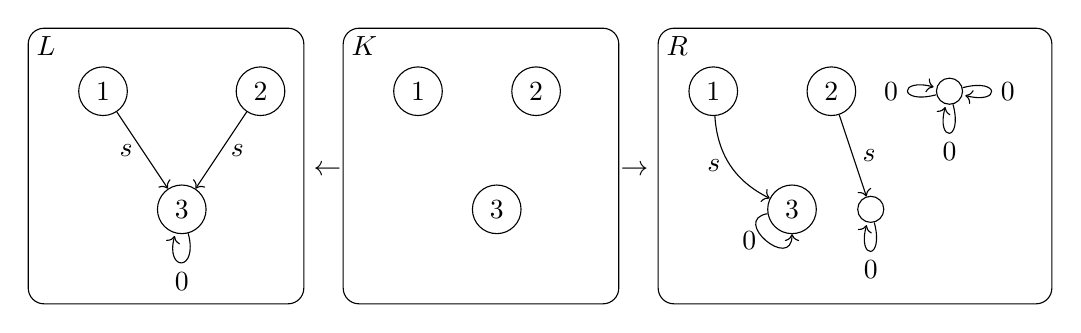
\begin{tikzpicture}
                \graphbox{$L$}{0mm}{0mm}{35mm}{35mm}{2mm}{-5mm}{
                    \coordinate (delta) at (0,-18mm);
                    \node[draw,circle] (l1) at ($(delta)+(-1,1.5)$) {1};
                    \node[draw,circle] (l2) at ($(delta)+(1,1.5)$) {2};
                    \node[draw,circle] (l3) at ($(delta)+(0,0)$) {3};
                    \draw[->] (l1) -- (l3) node[midway,left] {$s$};
                    \draw[->] (l2) -- (l3) node[midway,right] {$s$};
                    \draw[->] (l3) edge [loop below] node {0} (l3);
                }
                    \graphbox{$K$}{40mm}{0mm}{35mm}{35mm}{2mm}{-5mm}{
                        \coordinate (delta) at (0,-18mm);
                        \coordinate (interfaceorigin) at ($(delta) +(5,0)$);
                        \node[draw,circle] (r1) at ($(delta) +(-1,1.5)$) {1};
                        \node[draw,circle] (r2) at ($(delta) +(0.5,1.5)$) {2};
                        \node[draw,circle] (r3) at ($(delta)+(0,0)$) {3};
                    } 
                    \node () at (38mm,-18mm) {$\leftarrow$};
                    \node () at (77mm,-18mm) {$\rightarrow$};
                \graphbox{$R$}{80mm}{0mm}{50mm}{35mm}{2mm}{-5mm}{
                    \coordinate (delta) at (-10mm,-18mm);
                    \node[draw,circle] (r1) at ($(delta)+(-1,1.5)$) {1};
                    \node[draw,circle] (r2) at ($(delta)+(0.5,1.5)$) {2};
                    \node[draw,circle] (r3) at ($(delta)+(0,0)$) {3};
                    \node[draw,circle] (r4) at ($(delta)+(1,0)$) {};
                    \draw[->] (r1) edge[bend right] node[midway,left] {$s$} (r3) ;
                    \draw[->] (r2) -- (r4) node[midway,right] {$s$};
                    \draw[->] (r4) edge [loop below] node {0} (r4);
                    
                    \draw[->] (r3) edge [out=190,in=270,looseness=3] node[midway,left] {0} (r3);
                    \node[draw,circle] (r5) at ($(r2)+(1.5,0)$) {};
                    \draw[->] (r5) edge [loop below] node {0} (r5);
                    \draw[->] (r5) edge [loop right] node {0} (r5);
                    \draw[->] (r5) edge [loop left] node {0} (r5);
                }
            \end{tikzpicture}
            }
    \end{center}
Type graph fails: existence of surjections from $R$ to $L$.

All existing automated methods fail.

 Remark: the number of occurrences of $L$ strictly decreases.
 
 \note{
    La méthode par graphe de type pondéré a une limitation importante: elle ne peut pas prouver la terminaison d'une règle si il existe une surjection de R vers L, comme dans cet exemple.

    Dans ce cas, toutes les méthodes automatisées existantes échouent.

    On remarque que le nombre d'occurrences de L diminue strictement à chaque application de la règle.
    Ça suggère qu'une approche basée sur le comptage de sous-graphes pourrait être utile.
 }
\end{frame}

\section{Toward Greater Power}
% \begin{frame}
%   \tableofcontents[currentsection,hideothersubsections]
% \end{frame}

\begin{frame}{Capability Improvement: Morphism Counting}
    Termination by interpretation 
    \newline\newline
    Parameter: graph $X$
    \newline\newline
    Interpretation:
        \vspace{-3mm}
        \begin{flalign*}
        G &\leadsto |\mathrm{morphisms}(X,G)| \in\mathbb{N}
        \end{flalign*}

    \note{
        On propose une nouvelle methode de termination par interpretation.

        Cette methode utilise un graphe X comme parametre.

        L'interpretation d'un graphe G est le nombre de morphismes de X vers G.

        Pour faciliter notre discussion, on va introduire une autre definition de systems de reécriture de graphe après avoir présenter le concept d'inclusion. 
    }
\end{frame}

\begin{frame}{Inclusions}
         \begin{center} 
            \resizebox{\textwidth}{!}{
                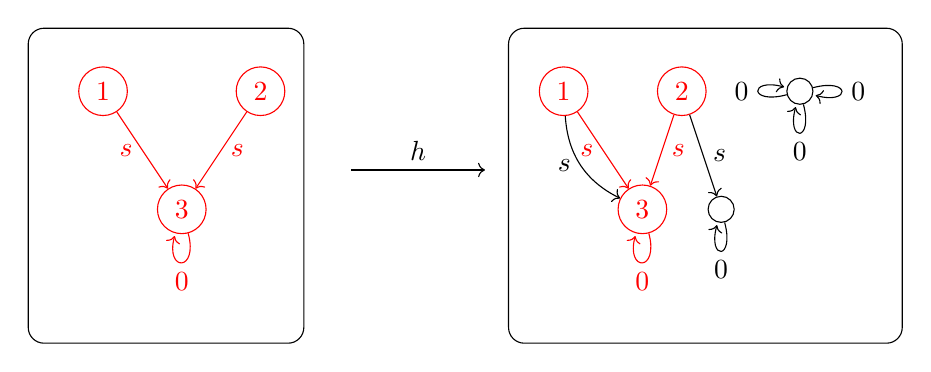
\begin{tikzpicture}
                    \graphbox{}{39mm}{0mm}{35mm}{40mm}{2mm}{-5mm}{
                        \coordinate (delta) at (0,-18mm);
                        \node[draw,circle,red] (l1) at ($(delta)+(-1,1.5)$) {1};
                        \node[draw,circle,red] (l2) at ($(delta)+(1,1.5)$) {2};
                        \node[draw,circle,red] (l3) at ($(delta)+(0,0)$) {3};
                        \draw[->,red] (l1) -- (l3) node[midway,left] {$s$};
                        \draw[->,red] (l2) -- (l3) node[midway,right] {$s$};
                        \draw[->,red] (l3) edge [loop below] node {0} (l3);
                    }
                        \draw[->] (80mm,-18mm) to node[midway,above] {$h$} (97mm,-18mm);
                    \graphbox{}{100mm}{0mm}{50mm}{40mm}{2mm}{-5mm}{
                        \coordinate (delta) at (-10mm,-18mm);
                        \node[draw,circle,red] (r1) at ($(delta)+(-1,1.5)$) {1};
                        \node[draw,circle,red] (r2) at ($(delta)+(0.5,1.5)$) {2};
                        \node[draw,circle,red] (r3) at ($(delta)+(0,0)$) {3};
                        \node[draw,circle] (r4) at ($(delta)+(1,0)$) {};
                        \node[draw,circle] (r5) at ($(r2)+(1.5,0)$) {};
                        \draw[->] (r1) edge[bend right] node[midway,left] {$s$} (r3) ; 
                        \draw[->] (r2) -- (r4) node[midway,right] {$s$};
                        \draw[->] (r4) edge [loop below] node {0} (r4);
                        \draw[->] (r5) edge [loop below] node {0} (r5);
                        \draw[->] (r5) edge [loop right] node {0} (r5);
                        \draw[->] (r5) edge [loop left] node {0} (r5);
                        \draw[->,red] (r1) edge node[midway,left] {$s$} (r3) ;
                        \draw[->,red] (r2) edge node[midway,right] {$s$} (r3) ; 
                        \draw[->,red] (r3) edge [loop below] node {0} (r3); 
                    }
                \end{tikzpicture}
                }
        \end{center}
 Subgraph
 \note{an inclusion is a morphism whose domain is a subgraph of its codomain and every node and edge in the domain is mapped to itself in the codomain.
 }
 
\end{frame}
 
\begin{frame}{Graph Rewriting Systems}
  A rewriting rules consists of two inclusions. 
  \begin{center}
    $\varphi$=\resizebox{0.78\textwidth}{!}{
      \begin{tikzpicture}[baseline=-10mm]
              \graphbox{\( L\)}{0mm}{5mm}{34mm}{15mm}{2mm}{0mm}{
                  \coordinate (o) at (0mm,-8mm); 
                  \node[draw,circle] (l1) at ($(o)+(-10mm,0mm)$) {6};
                  \node[draw,circle] (l2) at ($(l1)+(2,0)$) {7};
                  \node[orange,draw,circle] (l3) at ($(l1)+(1,0)$) {8};
                  \draw[orange,->] (l1) -- (l3) node[midway,above] {$a$};
                  \draw[orange,->] (l3) -- (l2) node[midway,above] {$a$};
              } 

              \graphbox{\( K \)}{40mm}{5mm}{34mm}{15mm}{2mm}{0mm}{
                  \coordinate (o) at (0mm,-8mm); 
                  \node[draw,circle] (l1) at ($(o)+(-10mm,0mm)$) {6};
                  \node[draw,circle] (l2) at ($(l1)+(2,0)$) {7};
              }  

              \graphbox{\( R \)}{80mm}{5mm}{45mm}{15mm}{2mm}{0mm}{
                  \coordinate (o) at (-5mm,-8mm); 
                  \node[draw,circle] (l1) at ($(o)+(-10mm,0mm)$) {6};
                  \node[draw,circle] (l2) at ($(l1)+(3,0)$) {7};
                  \node[red,draw,circle] (l3) at ($(l1)+(1,0)$) {9};
                  \node[red,draw,circle] (l4) at ($(l1)+(2,0)$) {10};
                  \draw[red,->] (l1) -- (l3) node[midway,above] {$a$};
                  \draw[red,->] (l3) -- (l4) node[midway,above] {$b$};
                  \draw[red,->] (l4) -- (l2) node[midway,above] {$a$};
              }    
              \node () at (37mm,-3mm) {\( \overset{l}{\leftarrow} \)}; % K -> L
              \node () at (77mm,-3mm) {\( \overset{r}{\rightarrow} \)}; % K -> R
      \end{tikzpicture}
      }
   \end{center}

   An equivalent rewriting rule expresses the same transformation. 

  \begin{center}
    $\varphi'$=\resizebox{0.78\textwidth}{!}{
      \begin{tikzpicture}[baseline=-10mm]
              \graphbox{\( L' \)}{0mm}{5mm}{34mm}{15mm}{2mm}{0mm}{
                  \coordinate (o) at (0mm,-8mm); 
                  \node[draw,circle] (l1) at ($(o)+(-10mm,0mm)$) {1};
                  \node[draw,circle] (l2) at ($(l1)+(2,0)$) {2};
                  \node[orange,draw,circle] (l3) at ($(l1)+(1,0)$) {3};
                  \draw[orange,->] (l1) -- (l3) node[midway,above] {$a$};
                  \draw[orange,->] (l3) -- (l2) node[midway,above] {$a$};
              } 

              \graphbox{\( K' \)}{40mm}{5mm}{34mm}{15mm}{2mm}{0mm}{
                  \coordinate (o) at (0mm,-8mm); 
                  \node[draw,circle] (l1) at ($(o)+(-10mm,0mm)$) {1};
                  \node[draw,circle] (l2) at ($(l1)+(2,0)$) {2};
              }  

              \graphbox{\( R' \)}{80mm}{5mm}{45mm}{15mm}{2mm}{0mm}{
                  \coordinate (o) at (-5mm,-8mm); 
                  \node[draw,circle] (l1) at ($(o)+(-10mm,0mm)$) {1};
                  \node[draw,circle] (l2) at ($(l1)+(3,0)$) {2};
                  \node[red,draw,circle] (l3) at ($(l1)+(1,0)$) {4};
                  \node[red,draw,circle] (l4) at ($(l1)+(2,0)$) {5};
                  \draw[red,->] (l1) -- (l3) node[midway,above] {$a$};
                  \draw[red,->] (l3) -- (l4) node[midway,above] {$b$};
                  \draw[red,->] (l4) -- (l2) node[midway,above] {$a$};
              }    
              \node () at (37mm,-3mm) {\( \overset{l'}{\leftarrow} \)}; 
              \node () at (77mm,-3mm) {\( \overset{r'}{\rightarrow} \)}; 
      \end{tikzpicture}
      }
   \end{center}
  
   A rewriting step with $\varphi$ is defined by a DPO diagram with inclusions and $\varphi'$.
  \begin{center}
    \resizebox{0.78\textwidth}{!}{
      \begin{tikzpicture}
              \graphbox{\( L' \)}{0mm}{5mm}{34mm}{15mm}{2mm}{0mm}{
                  \coordinate (o) at (0mm,-8mm); 
                  \node[draw,circle] (l1) at ($(o)+(-10mm,0mm)$) {1};
                  \node[draw,circle] (l2) at ($(l1)+(2,0)$) {2};
                  \node[orange,draw,circle] (l3) at ($(l1)+(1,0)$) {3};
                  \draw[orange,->] (l1) -- (l3) node[midway,above] {$a$};
                  \draw[orange,->] (l3) -- (l2) node[midway,above] {$a$};
              } 

              \graphbox{\( K' \)}{40mm}{5mm}{34mm}{15mm}{2mm}{0mm}{
                  \coordinate (o) at (0mm,-8mm); 
                  \node[draw,circle] (l1) at ($(o)+(-10mm,0mm)$) {1};
                  \node[draw,circle] (l2) at ($(l1)+(2,0)$) {2};
              }  

              \graphbox{\( R' \)}{80mm}{5mm}{45mm}{15mm}{2mm}{0mm}{
                  \coordinate (o) at (-5mm,-8mm); 
                  \node[draw,circle] (l1) at ($(o)+(-10mm,0mm)$) {1};
                  \node[draw,circle] (l2) at ($(l1)+(3,0)$) {2};
                  \node[red,draw,circle] (l3) at ($(l1)+(1,0)$) {4};
                  \node[red,draw,circle] (l4) at ($(l1)+(2,0)$) {5};
                  \draw[red,->] (l1) -- (l3) node[midway,above] {$a$};
                  \draw[red,->] (l3) -- (l4) node[midway,above] {$b$};
                  \draw[red,->] (l4) -- (l2) node[midway,above] {$a$};
              }    
                \graphbox{\( G  \)}{0mm}{-17mm}{34mm}{25mm}{2mm}{-5mm}{
                  \coordinate (o) at (0mm,-3mm); 
                  \node[draw,circle] (l1) at ($(o)+(-10mm,0mm)$) {1};
                  \node[draw,circle] (l2) at ($(l1)+(2,0)$) {2};
                  \node[draw,circle,orange] (l3) at ($(l1)+(1,0)$) {3};
                  \node[blue, draw,circle] (l4) at ($(l2)+(0,-1)$) {6};
                  \draw[orange,->] (l1) -- (l3) node[midway,above] {$a$};
                  \draw[orange,->] (l3) -- (l2) node[midway,above] {$a$};
                  \draw[blue,->] (l2) -- (l4) node[midway,right] {$a$};
              }    
              \graphbox{\( C  \)}{40mm}{-17mm}{34mm}{25mm}{2mm}{-5mm}{
                  \coordinate (o) at (0mm,-3mm); 
                  \node[draw,circle] (l1) at ($(o)+(-10mm,0mm)$) {1};
                  \node[draw,circle] (l2) at ($(l1)+(2,0)$) {2};
                  \node[blue,draw,circle] (l4) at ($(l2)+(0,-1)$) {6};
                  \draw[blue,->] (l2) -- (l4) node[midway,right] {$a$};
              }    
              \graphbox{\( H   \)}{80mm}{-17mm}{45mm}{25mm}{2mm}{-5mm}{
                  \coordinate (o) at (-5mm,-3mm); 
                  \node[draw,circle] (l1) at ($(o)+(-10mm,0mm)$) {1};
                  \node[draw,circle] (l2) at ($(l1)+(3,0)$) {2};
                  \node[draw,circle,red] (l3) at ($(l1)+(1,0)$) {4};
                  \node[draw,circle,red] (l4) at ($(l1)+(2,0)$) {5};
                  \node[blue,draw,circle] (l5) at ($(l2)+(0,-1)$) {6};
                  \draw[red,->] (l1) -- (l3) node[midway,above] {$a$};
                  \draw[red,->] (l3) -- (l4) node[midway,above] {$b$};
                  \draw[red,->] (l4) -- (l2) node[midway,above] {$a$};
                  \draw[blue,->] (l2) -- (l5) node[midway,right] {$a$};
              }    
              \node () at (37mm,-3mm) {\( \overset{l'}{\leftarrow} \)}; 
              \node () at (77mm,-3mm) {\( \overset{r'}{\rightarrow} \)}; 
              \node () at (17mm,-13mm) {\( \downarrow \)};
              \node () at (37mm,-28mm) {\( \leftarrow \)};
              \node () at (52mm,-13mm) {\( \downarrow \)};
              \node () at (92mm,-13mm) {\( \downarrow \)};
              \node () at (77mm,-28mm) {\( \rightarrow \)};  
      \end{tikzpicture}
      }
   \end{center}
   \note{
    Une règle de reécriture de graphes consiste en deux inclusions.

    Deux règles sont équivalentes si elles expriment la même transformation.

    Une étape de reécriture avec une règle est définie par un diagramme de double pushout avec des inclusions et une règle équivalente en haut. 

    Afin de faciliter la discussion, on va introduire le concept de pré-graphe.
   }
\end{frame}

\begin{frame}{Pre-Graphs}
  \noindent Graph:
         \begin{center}
            \resizebox{0.5\textwidth}{!}{
            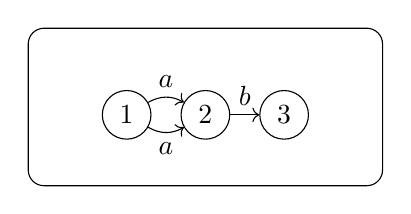
\begin{tikzpicture}
                \graphbox{}{0mm}{-20mm}{45mm}{20mm}{5mm}{-3mm}{ 
                    \coordinate (o) at (-5mm,-8mm); 
                    \node[draw,circle] (l1) at ($(o)+(-10mm,0mm)$) {1};
                    \node[draw,circle] (l3) at ($(l1)+(1,0)$) {2};
                    \node[draw,circle] (l4) at ($(l1)+(2,0)$) {3};
                    \draw[->] (l1) edge[bend right]  node[midway,below] {$a$} (l3);
                    \draw[->] (l1) edge[bend left] node[midway,above] {$a$}  (l3);
                    \draw[->] (l3) -- (l4) node[midway,above] {$b$};
                }  
            \end{tikzpicture} 
        }
        \end{center} 
    \begin{beamercolorbox}[rounded=true,shadow=true,wd=\textwidth]{block body}
    \noindent Pre-graphs obtained by removing node 2:
    \end{beamercolorbox}
        \begin{center}
            \resizebox{0.5\textwidth}{!}{
            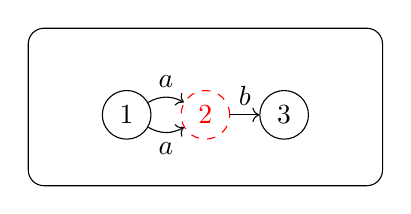
\begin{tikzpicture}
                \graphbox{}{0mm}{-20mm}{45mm}{20mm}{5mm}{-3mm}{ 
                    \coordinate (o) at (-5mm,-8mm); 
                    \node[draw,circle] (l1) at ($(o)+(-10mm,0mm)$) {1};
                    \node[draw,circle,dashed,red] (l3) at ($(l1)+(1,0)$) {2};
                    \node[draw,circle] (l4) at ($(l1)+(2,0)$) {3};
                    \draw[->] (l1) edge[bend right]  node[midway,below] {$a$} (l3);
                    \draw[->] (l1) edge[bend left] node[midway,above] {$a$}  (l3);
                    \draw[->] (l3) -- (l4) node[midway,above] {$b$};
                }  
            \end{tikzpicture} 
        }
        \end{center} 
 All edges are dangling.
 \note{
    Un pregraph est donc un graphe où certaines arêtes peuvent être pendantes.
    Par example, en supprimant le noeud 2 du graphe en haut, on obtient un pré-graphe en bas où toutes les arêtes sont pendantes.
 }
\end{frame}
\begin{frame}{Decomposition of Graphs in Rewriting Rules}
    \begin{center}
    \resizebox{0.85\textwidth}{!}{
      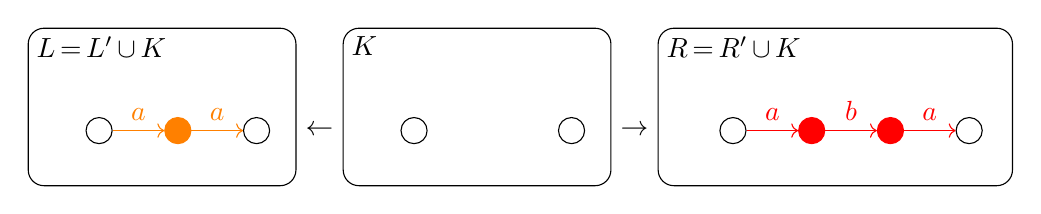
\begin{tikzpicture}
              \graphbox{\( L \mathop{=} L' \mathop{\cup} K \)}{0mm}{5mm}{34mm}{20mm}{2mm}{-5mm}{
                  \coordinate (o) at (0mm,-8mm); 
                  \node[draw,circle] (l1) at ($(o)+(-10mm,0mm)$) {};
                  \node[draw,circle] (l2) at ($(l1)+(2,0)$) {};
                  \node[orange,fill=orange,draw,circle] (l3) at ($(l1)+(1,0)$) {};
                  \draw[orange,fill=orange,->] (l1) -- (l3) node[midway,above] {$a$};
                  \draw[orange,fill=orange,->] (l3) -- (l2) node[midway,above] {$a$};
              } 

              \graphbox{\( K \)}{40mm}{5mm}{34mm}{20mm}{2mm}{-5mm}{
                  \coordinate (o) at (0mm,-8mm); 
                  \node[draw,circle] (l1) at ($(o)+(-10mm,0mm)$) {};
                  \node[draw,circle] (l2) at ($(l1)+(2,0)$) {};
              }  

              \graphbox{\( R \mathop{=} R' \mathop{\cup} K \)}{80mm}{5mm}{45mm}{20mm}{2mm}{-5mm}{
                  \coordinate (o) at (-5mm,-8mm); 
                  \node[draw,circle] (l1) at ($(o)+(-10mm,0mm)$) {};
                  \node[draw,circle] (l2) at ($(l1)+(3,0)$) {};
                  \node[red,fill=red,draw,circle] (l3) at ($(l1)+(1,0)$) {};
                  \node[red,fill=red,draw,circle] (l4) at ($(l1)+(2,0)$) {};
                  \draw[red,fill=red,->] (l1) -- (l3) node[midway,above] {$a$};
                  \draw[red,fill=red,->] (l3) -- (l4) node[midway,above] {$b$};
                  \draw[red,fill=red,->] (l4) -- (l2) node[midway,above] {$a$};
              }    

              \node () at (37mm,-8mm) {\( \leftarrow \)}; % K -> L
              \node () at (77mm,-8mm) {\( \rightarrow \)}; % K -> R
      \end{tikzpicture}
      }
   \end{center}
\begin{center}
    \resizebox{0.85\textwidth}{!}{
            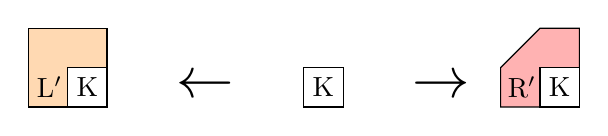
\begin{tikzpicture} 
                \coordinate (k) at (0, 0);
                \draw[fill=white] ($(k)+(0,0)$) rectangle ($(k)+(0.5,0.5)$);
                \node () at ($(k)+(0.25,0.25)$) {\( \mathrm{K} \)};
            
                \coordinate (l) at (-3, 0);
                \draw[fill=orange!30] ($(l)+(-0.5,0)$) rectangle ($(l)+(0.5,1)$);
                \node () at ($(l)+(-0.23,0.25)$) {\( \mathrm{L'} \)};
                \draw[fill=white] ($(l)+(0,0)$) rectangle ($(l)+(0.5,0.5)$);
                \node () at ($(l)+(0.25,0.25)$) {\( \mathrm{K} \)};
             
                \coordinate (r) at (3,0);
                \draw[fill=red!30] ($(r)+(-0.5,0)$)
                -- ($(r)+(-0.5,0.5)$)
                -- ($(r)+(0,1)$)
                --  ($(r)+(0.5,1)$)
                -- ($(r)+(0.5,0)$)
                -- cycle;
                \node () at ($(r)+(-0.23,0.25)$) {\( \mathrm{R'} \)};
                \draw[fill=white] ($(r)+(0,0)$) rectangle ($(r)+(0.5,0.5)$);
                \node () at ($(r)+(0.25,0.25)$) {\( \mathrm{K} \)};
             
                \node[ font=\huge] (kl) at ($(k)!0.5!(l)+(0.25,0.25)$)
                {\( \leftarrow \)}
                ; 
                \node[ font=\huge] (kr) at ($(k)!0.5!(r)+(0.25,0.25)$)
                {\( \rightarrow \)}
                ;  
            \end{tikzpicture}
          }
   \end{center}
   \note{
    Pour une règle de reécriture donnée, on peut décomposer le graph L comme l'union du graphe K et un autre pre-graphe L'. Pareil pour R.
    On peut représenter cette décomposition de manière plus abstraite comme dans le diagramme en bas. 

   }
\end{frame}
\begin{frame}{Decomposition of Graphs in Rewriting Steps}
   \begin{center}
    \resizebox{0.85\textwidth}{!}{
      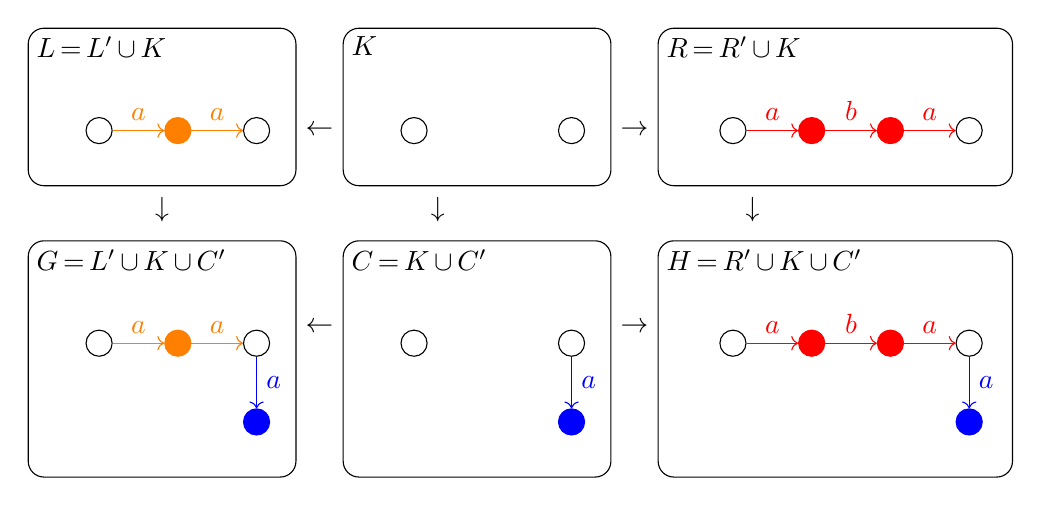
\begin{tikzpicture}
              \graphbox{\( L \mathop{=} L' \mathop{\cup} K \)}{0mm}{5mm}{34mm}{20mm}{2mm}{-5mm}{
                  \coordinate (o) at (0mm,-8mm); 
                  \node[draw,circle] (l1) at ($(o)+(-10mm,0mm)$) {};
                  \node[draw,circle] (l2) at ($(l1)+(2,0)$) {};
                  \node[orange,fill=orange,draw,circle] (l3) at ($(l1)+(1,0)$) {};
                  \draw[orange,fill=orange,->] (l1) -- (l3) node[midway,above] {$a$};
                  \draw[orange,fill=orange,->] (l3) -- (l2) node[midway,above] {$a$};
              } 

              \graphbox{\( K \)}{40mm}{5mm}{34mm}{20mm}{2mm}{-5mm}{
                  \coordinate (o) at (0mm,-8mm); 
                  \node[draw,circle] (l1) at ($(o)+(-10mm,0mm)$) {};
                  \node[draw,circle] (l2) at ($(l1)+(2,0)$) {};
              }  

              \graphbox{\( R \mathop{=} R' \mathop{\cup} K \)}{80mm}{5mm}{45mm}{20mm}{2mm}{-5mm}{
                  \coordinate (o) at (-5mm,-8mm); 
                  \node[draw,circle] (l1) at ($(o)+(-10mm,0mm)$) {};
                  \node[draw,circle] (l2) at ($(l1)+(3,0)$) {};
                  \node[red,fill=red,draw,circle] (l3) at ($(l1)+(1,0)$) {};
                  \node[red,fill=red,draw,circle] (l4) at ($(l1)+(2,0)$) {};
                  \draw[red,fill=red,->] (l1) -- (l3) node[midway,above] {$a$};
                  \draw[red,fill=red,->] (l3) -- (l4) node[midway,above] {$b$};
                  \draw[red,fill=red,->] (l4) -- (l2) node[midway,above] {$a$};
              }    

              \graphbox{\( G \mathop{=} L' \mathop{\cup} K \mathop{\cup} C' \)}{0mm}{-22mm}{34mm}{30mm}{2mm}{-10mm}{
                  \coordinate (o) at (0mm,-3mm); 
                  \node[draw,circle] (l1) at ($(o)+(-10mm,0mm)$) {};
                  \node[draw,circle] (l2) at ($(l1)+(2,0)$) {};
                  \node[draw,circle,orange,fill=orange] (l3) at ($(l1)+(1,0)$) {};
                  \node[blue, fill=blue,draw,circle] (l4) at ($(l2)+(0,-1)$) {};
                  \draw[orange,fill=orange,->] (l1) -- (l3) node[midway,above] {$a$};
                  \draw[orange,fill=orange,->] (l3) -- (l2) node[midway,above] {$a$};
                  \draw[blue,fill=blue,->] (l2) -- (l4) node[midway,right] {$a$};
              }    

              \graphbox{\( C \mathop{=} K \mathop{\cup} C' \)}{40mm}{-22mm}{34mm}{30mm}{2mm}{-10mm}{
                  \coordinate (o) at (0mm,-3mm); 
                  \node[draw,circle] (l1) at ($(o)+(-10mm,0mm)$) {};
                  \node[draw,circle] (l2) at ($(l1)+(2,0)$) {};
                  \node[blue,fill=blue,draw,circle] (l4) at ($(l2)+(0,-1)$) {};
                  \draw[blue,fill=blue,->] (l2) -- (l4) node[midway,right] {$a$};
              }    

              \graphbox{\( H \mathop{=} R' \mathop{\cup} K \mathop{\cup} C' \)}{80mm}{-22mm}{45mm}{30mm}{2mm}{-10mm}{
                  \coordinate (o) at (-5mm,-3mm); 
                  \node[draw,circle] (l1) at ($(o)+(-10mm,0mm)$) {};
                  \node[draw,circle] (l2) at ($(l1)+(3,0)$) {};
                  \node[red,fill=red,draw,circle] (l3) at ($(l1)+(1,0)$) {};
                  \node[red,fill=red,draw,circle] (l4) at ($(l1)+(2,0)$) {};
                  \node[blue,fill=blue,draw,circle] (l5) at ($(l2)+(0,-1)$) {};
                  \draw[red,fill=red,->] (l1) -- (l3) node[midway,above] {$a$};
                  \draw[red,fill=red,->] (l3) -- (l4) node[midway,above] {$b$};
                  \draw[red,fill=red,->] (l4) -- (l2) node[midway,above] {$a$};
                  \draw[blue,fill=blue,->] (l2) -- (l5) node[midway,right] {$a$};
              }    

              \node () at (37mm,-8mm) {\( \leftarrow \)}; % K -> L
              \node () at (77mm,-8mm) {\( \rightarrow \)}; % K -> R
              \node () at (17mm,-18mm) {\( \downarrow \)};
              \node () at (37mm,-33mm) {\( \leftarrow \)};
              \node () at (52mm,-18mm) {\( \downarrow \)};
              \node () at (92mm,-18mm) {\( \downarrow \)};
              \node () at (77mm,-33mm) {\( \rightarrow \)}; % C -> H
      \end{tikzpicture}
      }
   \end{center}
\begin{center}
    \resizebox{0.55\textwidth}{!}{
            \begin{tikzpicture} 
                \coordinate (k) at (0, 0);
                \draw[fill=white] ($(k)+(0,0)$) rectangle ($(k)+(0.5,0.5)$);
                \node () at ($(k)+(0.25,0.25)$) {\( \mathrm{K} \)};
            
                \coordinate (c) at (0, -2.2);
                \draw[fill=blue!30]
                ($(c)+(0,-0.5)$)
                -- ($(c)+(0,0.5)$) 
                -- ($(c)+(1,0.5)$) 
                arc[start angle=0, end angle=-90, radius=1]
                -- cycle;
                \node () at ($(c)+(0.75,0.25)$) {\( \mathrm{C'} \)};
                \draw[fill=white] ($(c)+(0,0)$) rectangle ($(c)+(0.5,0.5)$);
                \node () at ($(c)+(0.25,0.25)$) {\( \mathrm{K} \)};
            
                \coordinate (l) at (-3, 0);
                \draw[fill=orange!30] ($(l)+(-0.5,0)$) rectangle ($(l)+(0.5,1)$);
                \node () at ($(l)+(-0.23,0.25)$) {\( \mathrm{L'} \)};
                \draw[fill=white] ($(l)+(0,0)$) rectangle ($(l)+(0.5,0.5)$);
                \node () at ($(l)+(0.25,0.25)$) {\( \mathrm{K} \)};
            
                \coordinate (g) at (-3, -2.2);
                \draw[fill=blue!30]
                ($(g)+(0,-0.5)$)
                -- ($(g)+(0,0.5)$)
                -- ($(g)+(1,0.5)$) 
                arc[start angle=0, end angle=-90, radius=1]
                -- cycle;
                \draw[fill=orange!30] ($(g)+(-0.5,0)$) rectangle ($(g)+(0.5,1)$);
                \node () at ($(g)+(0.75,0.25)$) {\( \mathrm{C'} \)};
                \node () at ($(g)+(-0.23,0.25)$) {\( \mathrm{L'} \)};
                \draw[fill=white] ($(g)+(0,0)$) rectangle ($(g)+(0.5,0.5)$);
                \node () at ($(g)+(0.25,0.25)$) {\( \mathrm{K} \)};
            
                \coordinate (r) at (3,0);
                \draw[fill=red!30] ($(r)+(-0.5,0)$)
                -- ($(r)+(-0.5,0.5)$)
                -- ($(r)+(0,1)$)
                --  ($(r)+(0.5,1)$)
                -- ($(r)+(0.5,0)$)
                -- cycle;
                \node () at ($(r)+(-0.23,0.25)$) {\( \mathrm{R'} \)};
                \draw[fill=white] ($(r)+(0,0)$) rectangle ($(r)+(0.5,0.5)$);
                \node () at ($(r)+(0.25,0.25)$) {\( \mathrm{K} \)};
            
                \coordinate (h) at (3, -2.2);
                \draw[fill=blue!30]
                ($(h)+(0,-0.5)$)
                -- ($(h)+(0,0.5)$)
                -- ($(h)+(1,0.5)$) 
                arc[start angle=0, end angle=-90, radius=1]
                -- cycle;
                \draw[fill=red!30] ($(h)+(-0.5,0)$)
                -- ($(h)+(-0.5,0.5)$)
                -- ($(h)+(0,1)$)
                --  ($(h)+(0.5,1)$)
                -- ($(h)+(0.5,0)$)
                -- cycle;
            \node () at ($(h)+(0.75,0.25)$) {\( \mathrm{C'} \)};
            \draw[fill=white] ($(h)+(0,0)$) rectangle ($(h)+(0.5,0.5)$);
            \node () at ($(h)+(0.25,0.25)$) {\( \mathrm{K} \)};
            \node () at ($(h)+(-0.23,0.25)$) {\( \mathrm{R'} \)};
            
                \node[ font=\huge] (kl) at ($(k)!0.5!(l)+(0.25,0.25)$)
                {\( \leftarrow \)}
                ; 
                \node[ font=\huge] (kr) at ($(k)!0.5!(r)+(0.25,0.25)$)
                {\( \rightarrow \)}
                ;  
                \node[ font=\huge] (cg) at ($(c)!0.5!(g)+(0.25,0.25)$) 
                {\( \leftarrow \)}
            ;  
                \node[ font=\huge] (ch) at ($(c)!0.5!(h)+(0.25,0.25)$)
                {\( \rightarrow \)}
            ; 
                \node[ font=\huge] (kc) at ($(k)!0.5!(c)+(0.2,0.4)$) {\( \downarrow \)}; 
                \node[ font=\huge] (lg) at ($(l)!0.5!(g)+(0.1,0.4)$) {\( \downarrow \)}; 
                \node[ font=\huge] (rh) at ($(r)!0.5!(h)+(0.1,0.4)$) {\( \downarrow \)}; 
            \end{tikzpicture}
          }
   \end{center}
   This coloring provides a classification of morphisms in rewriting steps by image node colors.
   \note{
    Dans une étape de reécriture, chaque graphe peut etre exprime comme l'union de pré-graphes, comme montre le diagramme en haut. Le cas abstract est represente en bas.

    On peut colorier les differents pré-graphes avec des couleurs différentes.
    Cette coloration fournit une classification intuitive des morphismes dans les étapes de reécriture par les couleurs des noeuds de leurs images.
   }
\end{frame}


\begin{frame}{$X$-occurrences by Image Node Colors}
     \begin{beamercolorbox}[rounded=true,shadow=true,wd=\textwidth]{block body}
        An $X$-occurrence is an injective morphism from $X$. 
    \end{beamercolorbox}
 \begin{center}
    \resizebox{0.49\textwidth}{!}{
            \begin{tikzpicture} 
                \coordinate (k) at (0, 0);
                \draw[fill=white] ($(k)+(0,0)$) rectangle ($(k)+(0.5,0.5)$);
                \node () at ($(k)+(0.25,0.25)$) {\( \mathrm{K} \)};
            
                \coordinate (c) at (0, -2.2);
                \draw[fill=blue!30]
                ($(c)+(0,-0.5)$)
                -- ($(c)+(0,0.5)$) 
                -- ($(c)+(1,0.5)$) 
                arc[start angle=0, end angle=-90, radius=1]
                -- cycle;
                \node () at ($(c)+(0.75,0.25)$) {\( \mathrm{C'} \)};
                \draw[fill=white] ($(c)+(0,0)$) rectangle ($(c)+(0.5,0.5)$);
                \node () at ($(c)+(0.25,0.25)$) {\( \mathrm{K} \)};
            
                \coordinate (l) at (-3, 0);
                \draw[fill=orange!30] ($(l)+(-0.5,0)$) rectangle ($(l)+(0.5,1)$);
                \node () at ($(l)+(-0.23,0.25)$) {\( \mathrm{L'} \)};
                \draw[fill=white] ($(l)+(0,0)$) rectangle ($(l)+(0.5,0.5)$);
                \node () at ($(l)+(0.25,0.25)$) {\( \mathrm{K} \)};
            
                \coordinate (g) at (-3, -2.2);
                \draw[fill=blue!30]
                ($(g)+(0,-0.5)$)
                -- ($(g)+(0,0.5)$)
                -- ($(g)+(1,0.5)$) 
                arc[start angle=0, end angle=-90, radius=1]
                -- cycle;
                \draw[fill=orange!30] ($(g)+(-0.5,0)$) rectangle ($(g)+(0.5,1)$);
                \node () at ($(g)+(0.75,0.25)$) {\( \mathrm{C'} \)};
                \node () at ($(g)+(-0.23,0.25)$) {\( \mathrm{L'} \)};
                \draw[fill=white] ($(g)+(0,0)$) rectangle ($(g)+(0.5,0.5)$);
                \node () at ($(g)+(0.25,0.25)$) {\( \mathrm{K} \)};
            
                \coordinate (r) at (3,0);
                \draw[fill=red!30] ($(r)+(-0.5,0)$)
                -- ($(r)+(-0.5,0.5)$)
                -- ($(r)+(0,1)$)
                --  ($(r)+(0.5,1)$)
                -- ($(r)+(0.5,0)$)
                -- cycle;
                \node () at ($(r)+(-0.23,0.25)$) {\( \mathrm{R'} \)};
                \draw[fill=white] ($(r)+(0,0)$) rectangle ($(r)+(0.5,0.5)$);
                \node () at ($(r)+(0.25,0.25)$) {\( \mathrm{K} \)};
            
                \coordinate (h) at (3, -2.2);
                \draw[fill=blue!30]
                ($(h)+(0,-0.5)$)
                -- ($(h)+(0,0.5)$)
                -- ($(h)+(1,0.5)$) 
                arc[start angle=0, end angle=-90, radius=1]
                -- cycle;
                \draw[fill=red!30] ($(h)+(-0.5,0)$)
                -- ($(h)+(-0.5,0.5)$)
                -- ($(h)+(0,1)$)
                --  ($(h)+(0.5,1)$)
                -- ($(h)+(0.5,0)$)
                -- cycle;
            \node () at ($(h)+(0.75,0.25)$) {\( \mathrm{C'} \)};
            \draw[fill=white] ($(h)+(0,0)$) rectangle ($(h)+(0.5,0.5)$);
            \node () at ($(h)+(0.25,0.25)$) {\( \mathrm{K} \)};
            \node () at ($(h)+(-0.23,0.25)$) {\( \mathrm{R'} \)};
            
                \node[ font=\huge] (kl) at ($(k)!0.5!(l)+(0.25,0.25)$)
            %    {\( \overset{l}{\leftarrow} \)}
                {\( \leftarrow \)}
                ; 
                \node[ font=\huge] (kr) at ($(k)!0.5!(r)+(0.25,0.25)$)
                {\( \rightarrow \)}
                ;  
                \node[ font=\huge] (cg) at ($(c)!0.5!(g)+(0.25,0.25)$) 
                {\( \leftarrow \)}
            ;  
                \node[ font=\huge] (ch) at ($(c)!0.5!(h)+(0.25,0.25)$)
                {\( \rightarrow \)}
            ; 
                \node[ font=\huge] (kc) at ($(k)!0.5!(c)+(0.2,0.4)$) {\( \downarrow \)}; 
            %   \node[ font=\LARGE] () at ($(l)!0.5!(g)+(0.5,0.4)$) {$m$}; 
                \node[ font=\huge] (lg) at ($(l)!0.5!(g)+(0.1,0.4)$) {\( \downarrow \)}; 
                \node[ font=\huge] (rh) at ($(r)!0.5!(h)+(0.1,0.4)$) {\( \downarrow \)}; 
            %   \node[ font=\LARGE] () at ($(r)!0.5!(h)+(0.55,0.4)$) {$m'$}; 
            %   \node[ font=\LARGE] () at ($(k)!0.5!(c)+(0.5,0.4)$) {$u$}; 
            \end{tikzpicture}
          }
   \end{center}

   $X$-occurrence are classified by the colors of their image nodes:
   \begin{itemize}
    \item \textcolor{black}{white}: only \textcolor{black}{white};
    \item \textcolor{orange}{orange}: only \textcolor{black}{white} and at least one \textcolor{orange}{orange};
    \item \textcolor{blue}{blue}: only \textcolor{black}{white} and at least one \textcolor{blue}{blue};
     \item \textcolor{red}{red}: only \textcolor{black}{white} and at least one \textcolor{red}{red};
    \item \textcolor{blue}{blue}-and-\textcolor{orange}{orange}: 
        at least one \textcolor{blue}{blue} and at least one \textcolor{orange}{orange};
    \item \textcolor{blue}{blue}-and-\textcolor{red}{red}:
        at least one \textcolor{blue}{blue} and at least one \textcolor{red}{red}
   \end{itemize}
    % \begin{itemize}
    %     \item \textcolor{black}{white}: only \textcolor{black}{white}
    %     \item \textcolor{orange}{orange}: only \textcolor{black}{white} and at least one \textcolor{orange}{orange}
    %     \item \textcolor{red}{red}: only \textcolor{black}{white} and at least one \textcolor{red}{red}
    %     \item \textcolor{blue}{blue}: only \textcolor{black}{white} and \textcolor{blue}{blue} nodes;
    %      \item \textcolor{blue}{blue}-and-\textcolor{orange}{orange}: 
    %          at least one \textcolor{blue}{blue} and at least one \textcolor{orange}{orange}
    %     \item \textcolor{blue}{blue}-and-\textcolor{red}{red}:
    %         at least one \textcolor{blue}{blue} and at least one \textcolor{red}{red}

    % \end{itemize}
    
    \note{
    On appelle X-occurrence un morphisme injectif depuis X.

    Si l'image contient seulement des noeuds blancs, on dit qu'il est blanche.
    Si l'image contient une seule couleur autre que le blanc, on qu'il est de cette couleur.
    Si l'image contient des noeuds de deux couleurs differentes autres que le blanc, on dit qu'il est de ces deux couleurs.
    }
\end{frame}

\begin{frame}{Morphisms by Image Node Colors}
Let $X$ be the graph 
\raisebox{2pt}{
            \scalebox{0.7}{\tikz[baseline=-0.5ex]{
            \node [draw,circle] (z) at (-1,0) {};
            \node [draw,circle] (x) at (0,0) {};
            \node[draw,circle] (y) at (1,0) {};
            \draw[->] (z)--(x) node[midway, above] {$a$};
            \draw[->] (x)--(y) node[midway, above] {$a$};
        }}}. 
  \begin{center}
        \resizebox{0.8\textwidth}{!}{
      \begin{tikzpicture}
              \graphbox{\(\)}{0mm}{5mm}{34mm}{15mm}{2mm}{-2mm}{
                  \coordinate (o) at (0mm,-8mm); 
                  \node[draw,circle] (l1) at ($(o)+(-10mm,0mm)$) {1};
                  \node[draw,circle] (l2) at ($(l1)+(2,0)$) {2};
                  \node[orange,draw,circle] (l3) at ($(l1)+(1,0)$) {3};
                  \draw[orange,->] (l1) -- (l3) node[midway,above] {$a$};
                  \draw[orange,->] (l3) -- (l2) node[midway,above] {$a$};
              } 

              \graphbox{\(\)}{40mm}{5mm}{34mm}{15mm}{2mm}{-2mm}{
                  \coordinate (o) at (0mm,-8mm); 
                  \node[draw,circle] (l1) at ($(o)+(-10mm,0mm)$) {1};
                  \node[draw,circle] (l2) at ($(l1)+(2,0)$) {2};
              }  

              \graphbox{\(\)}{80mm}{5mm}{45mm}{15mm}{2mm}{-2mm}{
                  \coordinate (o) at (-5mm,-8mm); 
                  \node[draw,circle] (l1) at ($(o)+(-10mm,0mm)$) {1};
                  \node[draw,circle] (l2) at ($(l1)+(3,0)$) {2};
                  \node[red,draw,circle] (l3) at ($(l1)+(1,0)$) {4};
                  \node[red,draw,circle] (l4) at ($(l1)+(2,0)$) {5};
                  \draw[red,->] (l1) -- (l3) node[midway,above] {$a$};
                  \draw[red,->] (l3) -- (l4) node[midway,above] {$b$};
                  \draw[red,->] (l4) -- (l2) node[midway,above] {$a$};
              }    

              \graphbox{\(\)}{0mm}{-17mm}{34mm}{25mm}{2mm}{-7mm}{
                  \coordinate (o) at (0mm,-3mm); 
                  \node[draw,circle] (l1) at ($(o)+(-10mm,0mm)$) {1};
                  \node[draw,circle] (l2) at ($(l1)+(2,0)$) {2};
                  \node[draw,circle,orange] (l3) at ($(l1)+(1,0)$) {3};
                  \node[blue, draw,circle] (l4) at ($(l2)+(0,-1)$) {6};
                  \draw[orange,->] (l1) -- (l3) node[midway,above] {$a$};
                  \draw[orange,->] (l3) -- (l2) node[midway,above] {$a$};
                  \draw[blue,->] (l2) -- (l4) node[midway,right] {$a$};
                  \node[blue,draw,circle] (l7) at ($(l4)+(-1,0)$) {7};
                  \draw[blue,->] (l4) -- (l7) node[midway,below] {$a$};
              }    

              \graphbox{\(\)}{40mm}{-17mm}{34mm}{25mm}{2mm}{-7mm}{
                  \coordinate (o) at (0mm,-3mm); 
                  \node[draw,circle] (l1) at ($(o)+(-10mm,0mm)$) {1};
                  \node[draw,circle] (l2) at ($(l1)+(2,0)$) {2};
                  \node[blue,draw,circle] (l4) at ($(l2)+(0,-1)$) {6};
                  \draw[blue,->] (l2) -- (l4) node[midway,right] {$a$};
                %   \node[blue,draw,circle] (l6) at ($(l1)+(0,-1)$) {7};
                %   \draw[blue,<-] (l1) -- (l6) node[midway,left] {$a$};
                    \node[blue,draw,circle] (l7) at ($(l4)+(-1,0)$) {7};
                  \draw[blue,->] (l4) -- (l7) node[midway,below] {$a$};
              }    

              \graphbox{\(\)}{80mm}{-17mm}{45mm}{25mm}{2mm}{-7mm}{
                  \coordinate (o) at (-5mm,-3mm); 
                  \node[draw,circle] (l1) at ($(o)+(-10mm,0mm)$) {1};
                  \node[draw,circle] (l2) at ($(l1)+(3,0)$) {2};
                  \node[draw,circle,red] (l3) at ($(l1)+(1,0)$) {4};
                  \node[draw,circle,red] (l4) at ($(l1)+(2,0)$) {5};
                  \node[blue,draw,circle] (l5) at ($(l2)+(0,-1)$) {6};
                %   \node[blue,draw,circle] (l6) at ($(l1)+(0,-1)$) {7};
                %   \draw[blue,<-] (l1) -- (l6) node[midway,left] {$a$};
                  \draw[red,->] (l1) -- (l3) node[midway,above] {$a$};
                  \draw[red,->] (l3) -- (l4) node[midway,above] {$b$};
                  \draw[red,->] (l4) -- (l2) node[midway,above] {$a$};
                  \draw[blue,->] (l2) -- (l5) node[midway,right] {$a$};
                        \node[blue,draw,circle] (l7) at ($(l5)+(-1,0)$) {7};
                  \draw[blue,->] (l5) -- (l7) node[midway,below] {$a$};
              }    

              \node () at (37mm,-3mm) {\( \leftarrow \)}; % K -> L
              \node () at (77mm,-3mm) {\( \rightarrow \)}; % K -> R
              \node () at (17mm,-13mm) {\( m\ \downarrow \)};
              \node () at (37mm,-30mm) {\( \leftarrow \)};
              \node () at (52mm,-13mm) {\( \downarrow \)};
              \node () at (92mm,-13mm) {\( \downarrow \)};
              \node () at (77mm,-30mm) {\( \rightarrow \)}; % C -> H
      \end{tikzpicture}
        }
    \end{center}

\textcolor{blue}{Blue} $X$-occurrence:  \resizebox{0.18\textwidth}{!}{
        \tikz[baseline=-0.5ex]{ 
            \node[draw,circle] (x) at (0,0) {2};  
            \node[blue,draw,circle] (y) at (1,0) {6};
            \node[blue,draw,circle] (z) at (2,0) {7};
            \draw[blue,->] (x) -- node[midway,above] {$a$} (y) ;
            \draw[blue,->] (y) -- node[midway,above] {$a$} (z) ;
        }
    } 

% \textcolor{orange}{Orange} $X$-occurrences:
%     \resizebox{0.18\textwidth}{!}{  
%         \tikz[baseline=-0.5ex]{ 
%             \node[draw,circle] (x) at (0,0) {1};  
%             \node[orange,draw,circle] (y) at (1,0) {3};
%             \node[draw,circle] (z) at (2,0) {2};
%             \draw[orange,->] (x) -- node[midway,above] {$a$} (y) ;
%             \draw[orange,->] (y) -- node[midway,above] {$a$} (z) ;
%         }
%     }

% \textcolor{blue}{Blue}-and-\textcolor{orange}{Orange} $X$-occurrences:
%      \resizebox{0.18\textwidth}{!}{
%         \tikz[baseline=-0.5ex]{ 
%             \node[orange,draw,circle] (x) at (0,0) {3};  
%             \node[draw,circle] (y) at (1,0) {2};
%             \node[blue,draw,circle] (z) at (2,0) {6};
%             \draw[orange,->] (x) -- node[midway,above] {$a$} (y) ;
%             \draw[blue,->] (y) -- node[midway,above] {$a$} (z) ;
%         } 
%     }

\textcolor{red}{Red} $X$-occurrences: none.

\textcolor{blue}{Blue}-and-\textcolor{red}{red} $X$-occurrences:
    \resizebox{0.18\textwidth}{!}{
        \tikz[baseline=-0.5ex]{ 
            \node[red,draw,circle] (x) at (0,0) {5};  
            \node[draw,circle] (y) at (1,0) {2};
            \node[blue,draw,circle] (z) at (2,0) {6};
            \draw[red,->] (x) -- node[midway,above] {$a$} (y) ;
            \draw[blue,->] (y) -- node[midway,above] {$a$} (z) ;
        }
    }

\note{ 
    Une nouvelle critere de termination peut etre établie en termes des occurrences depuis un graphe X. 
}
\end{frame}


\begin{frame}{A New Sufficient Condition for Termination~\cite{qiu2025termination_icgt}}
    \begin{center}
    \resizebox{0.5\textwidth}{!}{
            \begin{tikzpicture} 
                \coordinate (k) at (0, 0);
                \draw[fill=white] ($(k)+(0,0)$) rectangle ($(k)+(0.5,0.5)$);
                \node () at ($(k)+(0.25,0.25)$) {\( \mathrm{K} \)};
            
                
                \coordinate (l) at (-3, 0);
                \draw[fill=orange!30] ($(l)+(-0.5,0)$) rectangle ($(l)+(0.5,1)$);
                \node () at ($(l)+(-0.23,0.25)$) {\( \mathrm{L'} \)};
                \draw[fill=white] ($(l)+(0,0)$) rectangle ($(l)+(0.5,0.5)$);
                \node () at ($(l)+(0.25,0.25)$) {\( \mathrm{K} \)};
            
                 
                \coordinate (r) at (3,0);
                \draw[fill=red!30] ($(r)+(-0.5,0)$)
                -- ($(r)+(-0.5,0.5)$)
                -- ($(r)+(0,1)$)
                --  ($(r)+(0.5,1)$)
                -- ($(r)+(0.5,0)$)
                -- cycle;
                \node () at ($(r)+(-0.23,0.25)$) {\( \mathrm{R'} \)};
                \draw[fill=white] ($(r)+(0,0)$) rectangle ($(r)+(0.5,0.5)$);
                \node () at ($(r)+(0.25,0.25)$) {\( \mathrm{K} \)};
            
                \node[ font=\huge] (kl) at ($(k)!0.5!(l)+(0.25,0.25)$)
                {\( \leftarrow \)}
                ; 
                \node[ font=\huge] (kr) at ($(k)!0.5!(r)+(0.25,0.25)$)
                {\( \rightarrow \)}
                ;  
            \end{tikzpicture}
          }
   \end{center}
    terminates if 
    \begin{itemize}
        \item strictly more \textcolor{orange}{orange} X-occurrences than \textcolor{red}{red} X-occurrences, 
        \item for every rewriting step:
    \begin{center}
    \resizebox{0.5\textwidth}{!}{
            \begin{tikzpicture} 
                \coordinate (k) at (0, 0);
                \draw[fill=white] ($(k)+(0,0)$) rectangle ($(k)+(0.5,0.5)$);
                \node () at ($(k)+(0.25,0.25)$) {\( \mathrm{K} \)};
                \coordinate (c) at (0, -2.2);
                \draw[fill=blue!30]
                ($(c)+(0,-0.5)$)
                -- ($(c)+(0,0.5)$) 
                -- ($(c)+(1,0.5)$) 
                arc[start angle=0, end angle=-90, radius=1]
                -- cycle;
                \node () at ($(c)+(0.75,0.25)$) {\( \mathrm{C'} \)};
                \draw[fill=white] ($(c)+(0,0)$) rectangle ($(c)+(0.5,0.5)$);
                \node () at ($(c)+(0.25,0.25)$) {\( \mathrm{K} \)};
            
                \coordinate (l) at (-3, 0);
                \draw[fill=orange!30] ($(l)+(-0.5,0)$) rectangle ($(l)+(0.5,1)$);
                \node () at ($(l)+(-0.23,0.25)$) {\( \mathrm{L'} \)};
                \draw[fill=white] ($(l)+(0,0)$) rectangle ($(l)+(0.5,0.5)$);
                \node () at ($(l)+(0.25,0.25)$) {\( \mathrm{K} \)};
            
                \coordinate (g) at (-3, -2.2);
                \draw[fill=blue!30]
                ($(g)+(0,-0.5)$)
                -- ($(g)+(0,0.5)$)
                -- ($(g)+(1,0.5)$) 
                arc[start angle=0, end angle=-90, radius=1]
                -- cycle;
                \draw[fill=orange!30] ($(g)+(-0.5,0)$) rectangle ($(g)+(0.5,1)$);
                \node () at ($(g)+(0.75,0.25)$) {\( \mathrm{C'} \)};
                \node () at ($(g)+(-0.23,0.25)$) {\( \mathrm{L'} \)};
                \draw[fill=white] ($(g)+(0,0)$) rectangle ($(g)+(0.5,0.5)$);
                \node () at ($(g)+(0.25,0.25)$) {\( \mathrm{K} \)};
            
                \coordinate (r) at (3,0);
                \draw[fill=red!30] ($(r)+(-0.5,0)$)
                -- ($(r)+(-0.5,0.5)$)
                -- ($(r)+(0,1)$)
                --  ($(r)+(0.5,1)$)
                -- ($(r)+(0.5,0)$)
                -- cycle;
                \node () at ($(r)+(-0.23,0.25)$) {\( \mathrm{R'} \)};
                \draw[fill=white] ($(r)+(0,0)$) rectangle ($(r)+(0.5,0.5)$);
                \node () at ($(r)+(0.25,0.25)$) {\( \mathrm{K} \)};
            
                \coordinate (h) at (3, -2.2);
                \draw[fill=blue!30]
                ($(h)+(0,-0.5)$)
                -- ($(h)+(0,0.5)$)
                -- ($(h)+(1,0.5)$) 
                arc[start angle=0, end angle=-90, radius=1]
                -- cycle;
                \draw[fill=red!30] ($(h)+(-0.5,0)$)
                -- ($(h)+(-0.5,0.5)$)
                -- ($(h)+(0,1)$)
                --  ($(h)+(0.5,1)$)
                -- ($(h)+(0.5,0)$)
                -- cycle;
            \node () at ($(h)+(0.75,0.25)$) {\( \mathrm{C'} \)};
            \draw[fill=white] ($(h)+(0,0)$) rectangle ($(h)+(0.5,0.5)$);
            \node () at ($(h)+(0.25,0.25)$) {\( \mathrm{K} \)};
            \node () at ($(h)+(-0.23,0.25)$) {\( \mathrm{R'} \)};
            
                \node[ font=\huge] (kl) at ($(k)!0.5!(l)+(0.25,0.25)$)
                {\( \leftarrow \)}
                ; 
                \node[ font=\huge] (kr) at ($(k)!0.5!(r)+(0.25,0.25)$)
                {\( \rightarrow \)}
                ;  
                \node[ font=\huge] (cg) at ($(c)!0.5!(g)+(0.25,0.25)$) 
                {\( \leftarrow \)}
            ;  
                \node[ font=\huge] (ch) at ($(c)!0.5!(h)+(0.25,0.25)$)
                {\( \rightarrow \)}
            ; 
                \node[ font=\huge] (kc) at ($(k)!0.5!(c)+(0.2,0.4)$) {\( \downarrow \)}; 
                \node[ font=\huge] (lg) at ($(l)!0.5!(g)+(0.1,0.4)$) {\( \downarrow \)}; 
                \node[ font=\huge] (rh) at ($(r)!0.5!(h)+(0.1,0.4)$) {\( \downarrow \)}; 
            \end{tikzpicture}
          }
   \end{center}
        has more \textcolor{blue}{blue}-and-\textcolor{orange}{orange} X-occurrences than \textcolor{blue}{blue}-and-\textcolor{red}{red} X-occurrences.
\end{itemize} 
    
 Challenge: check the second condition under the unknown C'
\end{frame} 

\begin{frame}{Analysis of Implicit Occurrences}
    \begin{center}
        \resizebox{\textwidth}{!}{
      \begin{tikzpicture}
              \graphbox{\(\)}{0mm}{5mm}{34mm}{20mm}{2mm}{-5mm}{
                  \coordinate (o) at (0mm,-8mm); 
                  \node[draw,circle] (l1) at ($(o)+(-10mm,0mm)$) {1};
                  \node[draw,circle] (l2) at ($(l1)+(2,0)$) {2};
                  \node[orange,draw,circle] (l3) at ($(l1)+(1,0)$) {3};
                  \draw[orange,->] (l1) -- (l3) node[midway,above] {$a$};
                  \draw[orange,->] (l3) -- (l2) node[midway,above] {$a$};
              } 

              \graphbox{\(\)}{40mm}{5mm}{34mm}{20mm}{2mm}{-5mm}{
                  \coordinate (o) at (0mm,-8mm); 
                  \node[draw,circle] (l1) at ($(o)+(-10mm,0mm)$) {1};
                  \node[draw,circle] (l2) at ($(l1)+(2,0)$) {2};
              }  

              \graphbox{\( \)}{80mm}{5mm}{45mm}{20mm}{2mm}{-5mm}{
                  \coordinate (o) at (-5mm,-8mm); 
                  \node[draw,circle] (l1) at ($(o)+(-10mm,0mm)$) {1};
                  \node[draw,circle] (l2) at ($(l1)+(3,0)$) {2};
                  \node[red,draw,circle] (l3) at ($(l1)+(1,0)$) {4};
                  \node[red,draw,circle] (l4) at ($(l1)+(2,0)$) {5};
                  \draw[red,->] (l1) -- (l3) node[midway,above] {$a$};
                  \draw[red,->] (l3) -- (l4) node[midway,above] {$b$};
                  \draw[red,->] (l4) -- (l2) node[midway,above] {$a$};
              }    

              \graphbox{\(   \)}{0mm}{-22mm}{34mm}{30mm}{2mm}{-10mm}{
                  \coordinate (o) at (0mm,-3mm); 
                  \node[draw,circle] (l1) at ($(o)+(-10mm,0mm)$) {1};
                  \node[draw,circle] (l2) at ($(l1)+(2,0)$) {2};
                  \node[draw,circle,orange] (l3) at ($(l1)+(1,0)$) {3};
                  \node[blue, draw,circle] (l4) at ($(l2)+(0,-1)$) {6};
                  \draw[orange,->] (l1) -- (l3) node[midway,above] {$a$};
                  \draw[orange,->] (l3) -- (l2) node[midway,above] {$a$};
                  \draw[blue,->] (l2) -- (l4) node[midway,right] {$a$};
                \node[blue,draw,circle] (l7) at ($(l4)+(-1,0)$) {7};
                  \draw[blue,->] (l4) -- (l7) node[midway,below] {$a$};
              }    

              \graphbox{\(  \)}{40mm}{-22mm}{34mm}{30mm}{2mm}{-10mm}{
                  \coordinate (o) at (0mm,-3mm); 
                  \node[draw,circle] (l1) at ($(o)+(-10mm,0mm)$) {1};
                  \node[draw,circle] (l2) at ($(l1)+(2,0)$) {2};
                  \node[blue,draw,circle] (l4) at ($(l2)+(0,-1)$) {6};
                  \draw[blue,->] (l2) -- (l4) node[midway,right] {$a$};
                    \node[blue,draw,circle] (l7) at ($(l4)+(-1,0)$) {7};
                  \draw[blue,->] (l4) -- (l7) node[midway,below] {$a$};
              }    

              \graphbox{\(   \)}{80mm}{-22mm}{45mm}{30mm}{2mm}{-10mm}{
                  \coordinate (o) at (-5mm,-3mm); 
                  \node[draw,circle] (l1) at ($(o)+(-10mm,0mm)$) {1};
                  \node[draw,circle] (l2) at ($(l1)+(3,0)$) {2};
                  \node[draw,circle,red] (l3) at ($(l1)+(1,0)$) {4};
                  \node[draw,circle,red] (l4) at ($(l1)+(2,0)$) {5};
                  \node[blue,draw,circle] (l5) at ($(l2)+(0,-1)$) {6};
                  \draw[red,->] (l1) -- (l3) node[midway,above] {$a$};
                  \draw[red,->] (l3) -- (l4) node[midway,above] {$b$};
                  \draw[red,->] (l4) -- (l2) node[midway,above] {$a$};
                  \draw[blue,->] (l2) -- (l5) node[midway,right] {$a$};
                        \node[blue,draw,circle] (l7) at ($(l5)+(-1,0)$) {7};
                  \draw[blue,->] (l5) -- (l7) node[midway,below] {$a$};
              }    

              \node () at (37mm,-8mm) {\( \leftarrow \)}; % K -> L
              \node () at (77mm,-8mm) {\( \rightarrow \)}; % K -> R
              \node () at (17mm,-18mm) {\( m\ \downarrow \)};
              \node () at (37mm,-33mm) {\( \leftarrow \)};
              \node () at (52mm,-18mm) {\( \downarrow \)};
              \node () at (92mm,-18mm) {\( \downarrow \)};
              \node () at (77mm,-33mm) {\( \rightarrow \)}; % C -> H
      \end{tikzpicture}
      }
    \end{center}
    \textcolor{blue}{Blue}-and-\textcolor{red}{red} $X$-occurrences:
    \resizebox{0.18\textwidth}{!}{
        \tikz[baseline=-0.5ex]{ 
            \node[red,draw,circle] (x) at (0,0) {5};  
            \node[draw,circle] (y) at (1,0) {2};
            \node[blue,draw,circle] (z) at (2,0) {6};
            \draw[red,->] (x) -- node[midway,above] {$a$} (y) ;
            \draw[blue,->] (y) -- node[midway,above] {$a$} (z) ;
        }
    }

    \textcolor{blue}{Blue}-and-\textcolor{orange}{Orange} $X$-occurrences:
     \resizebox{0.18\textwidth}{!}{
        \tikz[baseline=-0.5ex]{ 
            \node[orange,draw,circle] (x) at (0,0) {3};  
            \node[draw,circle] (y) at (1,0) {2};
            \node[blue,draw,circle] (z) at (2,0) {6};
            \draw[orange,->] (x) -- node[midway,above] {$a$} (y) ;
            \draw[blue,->] (y) -- node[midway,above] {$a$} (z) ;
        } 
    }
\end{frame}

\begin{frame}{Sufficient Condition for the Second Condition~\cite{qiu2025termination_icgt}}
    \begin{center}
        \begin{tikzpicture} 
            \coordinate (k) at (0, 0);
            \draw[fill=white] ($(k)+(0,0)$) rectangle ($(k)+(0.5,0.5)$);
            \node () at ($(k)+(0.25,0.25)$) {\( \mathrm{K} \)};
        
            \coordinate (c) at (0, -2.2);
            \draw[fill=blue!30]
            ($(c)+(0,-0.5)$)
            -- ($(c)+(0,0.5)$) 
            -- ($(c)+(1,0.5)$) 
            arc[start angle=0, end angle=-90, radius=1]
            -- cycle;
            \node () at ($(c)+(0.75,0.25)$) {\( \mathrm{C'} \)};
            \draw[fill=white] ($(c)+(0,0)$) rectangle ($(c)+(0.5,0.5)$);
            \node () at ($(c)+(0.25,0.25)$) {\( \mathrm{K} \)};
        
            \coordinate (l) at (-3, 0);
            \draw[fill=orange!30] ($(l)+(-0.5,0)$) rectangle ($(l)+(0.5,1)$);
            \node () at ($(l)+(-0.23,0.25)$) {\( \mathrm{L'} \)};
            \draw[fill=white] ($(l)+(0,0)$) rectangle ($(l)+(0.5,0.5)$);
            \node () at ($(l)+(0.25,0.25)$) {\( \mathrm{K} \)};
        
            \coordinate (g) at (-3, -2.2);
            \draw[fill=blue!30]
            ($(g)+(0,-0.5)$)
            -- ($(g)+(0,0.5)$)
            -- ($(g)+(1,0.5)$) 
            arc[start angle=0, end angle=-90, radius=1]
            -- cycle;
            \draw[fill=orange!30] ($(g)+(-0.5,0)$) rectangle ($(g)+(0.5,1)$);
            \node () at ($(g)+(0.75,0.25)$) {\( \mathrm{C'} \)};
            \node () at ($(g)+(-0.23,0.25)$) {\( \mathrm{L'} \)};
            \draw[fill=white] ($(g)+(0,0)$) rectangle ($(g)+(0.5,0.5)$);
            \node () at ($(g)+(0.25,0.25)$) {\( \mathrm{K} \)};
        
            \coordinate (r) at (3,0);
            \draw[fill=red!30] ($(r)+(-0.5,0)$)
            -- ($(r)+(-0.5,0.5)$)
            -- ($(r)+(0,1)$)
            --  ($(r)+(0.5,1)$)
            -- ($(r)+(0.5,0)$)
            -- cycle;
            \node () at ($(r)+(-0.23,0.25)$) {\( \mathrm{R'} \)};
            \draw[fill=white] ($(r)+(0,0)$) rectangle ($(r)+(0.5,0.5)$);
            \node () at ($(r)+(0.25,0.25)$) {\( \mathrm{K} \)};
        
            \coordinate (h) at (3, -2.2);
            \draw[fill=blue!30]
            ($(h)+(0,-0.5)$)
            -- ($(h)+(0,0.5)$)
            -- ($(h)+(1,0.5)$) 
            arc[start angle=0, end angle=-90, radius=1]
            -- cycle;
            \draw[fill=red!30] ($(h)+(-0.5,0)$)
            -- ($(h)+(-0.5,0.5)$)
            -- ($(h)+(0,1)$)
            --  ($(h)+(0.5,1)$)
            -- ($(h)+(0.5,0)$)
            -- cycle;
        \node () at ($(h)+(0.75,0.25)$) {\( \mathrm{C'} \)};
        \draw[fill=white] ($(h)+(0,0)$) rectangle ($(h)+(0.5,0.5)$);
        \node () at ($(h)+(0.25,0.25)$) {\( \mathrm{K} \)};
        \node () at ($(h)+(-0.23,0.25)$) {\( \mathrm{R'} \)};
        
            \node[ font=\huge] (kl) at ($(k)!0.5!(l)+(0.25,0.25)$)
            {\( \leftarrow \)}
            ; 
            \node[ font=\huge] (kr) at ($(k)!0.5!(r)+(0.25,0.25)$)
            {\( \rightarrow \)}
            ;  
            \node[ font=\huge] (cg) at ($(c)!0.5!(g)+(0.25,0.25)$) 
            {\( \leftarrow \)}
        ;  
            \node[ font=\huge] (ch) at ($(c)!0.5!(h)+(0.25,0.25)$)
            {\( \rightarrow \)}
        ; 
            \node[ font=\huge] (kc) at ($(k)!0.5!(c)+(0.2,0.4)$) {\( \downarrow \)}; 
            \node[ font=\huge] (lg) at ($(l)!0.5!(g)+(0.1,0.4)$) {\( \downarrow \)}; 
            \node[ font=\huge] (rh) at ($(r)!0.5!(h)+(0.1,0.4)$) {\( \downarrow \)}; 
        \end{tikzpicture}
    \end{center}
    \begin{beamercolorbox}[rounded=true,shadow=true,wd=\textwidth]{block body}
        There are more \textcolor{blue}{blue}-and-\textcolor{orange}{orange} X-morphisms than \textcolor{blue}{blue}-and-\textcolor{red}{red} X-morphisms,
        if  all subgraphs of \resizebox{0.1\textwidth}{!}{
                \begin{tikzpicture}[baseline=1.5ex]
                    \coordinate (r) at (3,0);
                    \draw[fill=red!30] ($(r)+(-0.5,0)$)
                    -- ($(r)+(-0.5,0.5)$)
                    -- ($(r)+(0,1)$)
                    --  ($(r)+(0.5,1)$)
                    -- ($(r)+(0.5,0)$)
                    -- cycle;
                    \node () at ($(r)+(-0.23,0.25)$) {\( \mathrm{R'} \)};
                    \draw[fill=white] ($(r)+(0,0)$) rectangle ($(r)+(0.5,0.5)$);
                    \node () at ($(r)+(0.25,0.25)$) {\( \mathrm{K} \)};
                \end{tikzpicture}
            } that can form an \textcolor{blue}{blue}-and-\textcolor{red}{red} $X$-occurrence in any rewriting step can be mapped to distinct  subgraphs in \resizebox{0.1\textwidth}{!}{
                \begin{tikzpicture}[baseline=1.5ex]
                    \coordinate (l) at (-3, 0);
                    \draw[fill=orange!30] ($(l)+(-0.5,0)$) rectangle ($(l)+(0.5,1)$);
                    \node () at ($(l)+(-0.23,0.25)$) {\( \mathrm{L'} \)};
                    \draw[fill=white] ($(l)+(0,0)$) rectangle ($(l)+(0.5,0.5)$);
                    \node () at ($(l)+(0.25,0.25)$) {\( \mathrm{K} \)};
                \end{tikzpicture}
 } while 
    preserving elements in \begin{tikzpicture}
        \coordinate (k) at (0, 0);
            \draw[fill=white] ($(k)+(0,0)$) rectangle ($(k)+(0.5,0.5)$);
            \node () at ($(k)+(0.25,0.25)$) {\( \mathrm{K} \)};
    \end{tikzpicture}.
    \end{beamercolorbox}
\end{frame} 
   

\begin{frame}{Termination of Motivating Example}
     \begin{center}
        \resizebox{\textwidth}{!}{ 
            \begin{tikzpicture}
                \graphbox{$L$}{0mm}{0mm}{35mm}{35mm}{2mm}{-5mm}{
                    \coordinate (delta) at (0,-18mm);
                    \node[draw,circle] (l1) at ($(delta)+(-1,1.5)$) {1};
                    \node[draw,circle] (l2) at ($(delta)+(1,1.5)$) {2};
                    \node[draw,circle] (l3) at ($(delta)+(0,0)$) {3};
                    \draw[->] (l1) -- (l3) node[midway,left] {$s$};
                    \draw[->] (l2) -- (l3) node[midway,right] {$s$};
                    \draw[->] (l3) edge [loop below] node {0} (l3);
                }
                    \graphbox{$K$}{40mm}{0mm}{35mm}{35mm}{2mm}{-5mm}{
                        \coordinate (delta) at (0,-18mm);
                        \coordinate (interfaceorigin) at ($(delta) +(5,0)$);
                        \node[draw,circle] (r1) at ($(delta) +(-1,1.5)$) {1};
                        \node[draw,circle] (r2) at ($(delta) +(0.5,1.5)$) {2};
                        \node[draw,circle] (r3) at ($(delta)+(0,0)$) {3};
                    } 
                    \node () at (38mm,-18mm) {$\leftarrow$};
                    \node () at (77mm,-18mm) {$\rightarrow$};
                \graphbox{$R$}{80mm}{0mm}{50mm}{35mm}{2mm}{-5mm}{
                    \coordinate (delta) at (-10mm,-18mm);
                    \node[draw,circle] (r1) at ($(delta)+(-1,1.5)$) {1};
                    \node[draw,circle] (r2) at ($(delta)+(0.5,1.5)$) {2};
                    \node[draw,circle] (r3) at ($(delta)+(0,0)$) {3};
                    \node[draw,circle] (r4) at ($(delta)+(1,0)$) {};
                    \draw[->] (r1) edge[bend right] node[midway,left] {$s$} (r3) ;
                    \draw[->] (r2) -- (r4) node[midway,right] {$s$};
                    \draw[->] (r4) edge [loop below] node {0} (r4);
                    
                    \draw[->] (r3) edge [out=190,in=270,looseness=3] node[midway,left] {0} (r3);
                    \node[draw,circle] (r5) at ($(r2)+(1.5,0)$) {};
                    \draw[->] (r5) edge [loop below] node {0} (r5);
                    \draw[->] (r5) edge [loop right] node {0} (r5);
                    \draw[->] (r5) edge [loop left] node {0} (r5);
                }
            \end{tikzpicture}
            }
    \end{center}

    Existing automated methods fail.

    Termination proved by counting morphisms from 
    $\tikz[baseline=-0.5ex]{ 
                \node[draw,circle] (x) at (0,0) {}; 
                \node[draw,circle] (y) at (1,0) {};
                \node[draw,circle] (z) at (2,0) {};
                \draw[->] (x) -- (y) node[midway, above] {$s$};
                \draw[->] (z) -- (y) node[midway, above] {$s$};
    }$.

\end{frame}

\begin{frame}{Imcomparable with Existing Methods}
\begin{tikzpicture}
    \node[draw,circle, minimum size=5cm] (n1) at (0,0) {Morphism Counting};
    \node[draw,circle, minimum size=5cm] (n2) at (4.5,0) {Existing Methods};
\end{tikzpicture}

Succeed in some cases where all existing automated methods fail.

Fail in some cases where other methods succeed.
\end{frame}

\section{LyonParallel—A Tool for Termination of
Graph Rewriting}

\begin{frame}{LyonParallel}
   \begin{description}
    \item[Automated tool in Ocaml]
    \item[Iterative elimination of graph rewriting rules]
    \item[Available : \url{https://github.com/Qi-tchi/LyonParallel}]
   \end{description}
\end{frame}


\begin{frame}{Process Flowchart of LyonParallel}
\centering
\tikzset{
  startstop/.style = {rectangle, rounded corners, draw, align=center, minimum width=2.8cm, minimum height=0.8cm},
  process/.style   = {rectangle, draw, align=center, minimum width=3.4cm, minimum height=0.8cm},
  decision/.style  = {diamond, draw, aspect=2, align=center, inner sep=2pt, minimum width=2.6cm},
  >=Stealth
}
\resizebox{\textwidth}{!}{
    \begin{tikzpicture}[node distance=8mm, auto]
  \node[draw, rounded corners, rectangle] (start) {Start program};
  \node[draw, rectangle, below=of start] (select) {Select graph rewriting system};
  \node[draw, diamond, aspect=2, below=of select] (choose) {Choose a method};

  % Two explicit methods
  \node[draw, rectangle, below left=8mm of choose] (typegraph) {\textcolor{red}{Type Graph Method}};
  \node[draw, rectangle, below right=8mm of choose] (subcount) {\textcolor{red}{Subgraph Counting}};

  % Z3 step (compact)
  \node[draw, rectangle, below=of typegraph] (z3) {Solve constraints with \textcolor{red}{Z3}};

  % Continue original flow
   \node[draw, diamond, aspect=2, below=22mm of choose] (check) {System simplified?};
  \node[draw, diamond, aspect=2, left=22mm of check] (trynext) {Try other method?};
  \node[draw, diamond, aspect=2, right=22mm of check] (empty) {Empty system?};
  \node[draw, rounded corners, rectangle, below=22mm of check] (end) {End};

  % Arrows (keep original structure)
  \draw[->] (start) -- (select);
  \draw[->] (select) -- (choose);

  % Branches to methods
  \draw[->] (choose) -- (typegraph);
  \draw[->] (choose) -- (subcount);

  % Method subflows back to apply
  \draw[->] (typegraph) -- (z3);
  % \draw[->] (z3.south) |- (apply.west);
  % \draw[->] (subcount.south) |- (apply.east);
    \draw[->] (z3.south) --  (check.north west);
  \draw[->] (subcount.south) -- (check.north east);

  % Main flow
  \draw[->] (check) -- node[midway,above]{Yes} (empty);
  \draw[->] (empty) |- node[midway,above]{No} (choose);
  \draw[->] (empty) -- node[midway,above]{Yes} (end);
  \draw[->] (check) -- node[midway,above]{No} (trynext);
  \draw[->] (trynext) |- node[midway,above]{Yes} (choose);
  \draw[->] (trynext) -- node[midway,left]{No} (end);
    \end{tikzpicture}
}
\end{frame}

\begin{frame}{Conclusion and Future Work}
  \textbf{Contributions}
  \begin{itemize}
    \item Extended the Weighted Type Graph Method to improve usability.
    \item Proposed a termination criterion applicable to new cases.
    \item Extended Morphism Counting to count morphisms with a forbidden context.
    \item Implemented an automated tool for termination analysis.
  \end{itemize}
    \vspace{4mm}
  \textbf{Future work}
  \begin{itemize}
    \item Short term: Morphism Counting with forbidden contexts.
    \item Mid term: Certificate-generation mechanism.
    \item Long term: Extension to other graph rewriting frameworks (e.g., PBPO+)
  \end{itemize}
\end{frame}

\begin{frame}[allowframebreaks]{References}
    \small % optional: make entries smaller
    \printbibliography
\end{frame} 

\begin{frame}{Pre-Graph Operations}
     \begin{beamercolorbox}[rounded=true,shadow=true,wd=\textwidth]{block body}
        \textcolor{red}{Union} of two pre-graphs $C \mathop{\subseteq} G$ and $R \mathop{\subseteq} G$, denoted $C \mathop{\cup} R$.
    \end{beamercolorbox}
\begin{center}
    \resizebox{\textwidth}{!}{
        \begin{tikzpicture}          
            \graphbox{\( C  \)}{0mm}{-22mm}{34mm}{25mm}{2mm}{-3mm}{
                \coordinate (o) at (0mm,-6mm); 
                \node[draw,circle,dashed] (l1) at ($(o)+(-10mm,0mm)$) {1};
                \node[draw,circle,dashed] (l2) at ($(l1)+(2,0)$) {2};
                \node[draw,circle] (l4) at ($(l2)+(0,-1)$) {6};
                \draw[->] (l2) -- (l4) node[midway,right] {$a$};
            }     
            \graphbox{\( R \)}{40mm}{-22mm}{45mm}{25mm}{2mm}{2mm}{
                \coordinate (o) at (-5mm,-8mm); 
                \node[draw,circle] (l1) at ($(o)+(-10mm,0mm)$) {1};
                \node[draw,circle] (l2) at ($(l1)+(3,0)$) {2};
                \node[draw,circle] (l3) at ($(l1)+(1,0)$) {4};
                \node[draw,circle] (l4) at ($(l1)+(2,0)$) {5};
                \draw[->] (l1) -- (l3) node[midway,above] {$a$};
                \draw[->] (l3) -- (l4) node[midway,above] {$b$};
                \draw[->] (l4) -- (l2) node[midway,above] {$a$};
            } 
            \graphbox{\textcolor{red}{\(C \mathop{\cup} R \)}}{91mm}{-22mm}{45mm}{25mm}{2mm}{-3mm}{
                \coordinate (o) at (-5mm,-6mm); 
                \node[draw,circle] (l1) at ($(o)+(-10mm,0mm)$) {1};
                \node[draw,circle] (l2) at ($(l1)+(3,0)$) {2};
                \node[draw,circle] (l3) at ($(l1)+(1,0)$) {4};
                \node[draw,circle] (l4) at ($(l1)+(2,0)$) {5};
                \node[ draw,circle] (l5) at ($(l2)+(0,-1)$) {6};
                \draw[->] (l1) -- (l3) node[midway,above] {$a$};
                \draw[->] (l3) -- (l4) node[midway,above] {$b$};
                \draw[->] (l4) -- (l2) node[midway,above] {$a$};
                \draw[->] (l2) -- (l5) node[midway,right] {$a$};
            }    
             
        \end{tikzpicture}
    }
    \end{center}
 \begin{beamercolorbox}[rounded=true,shadow=true,wd=\textwidth]{block body}
     \textcolor{red}{Relative complement} of $R$ in $H$ where $R \mathop{\subseteq} H$, denoted $H \mathop{\setminus} R$.
\end{beamercolorbox}
    \begin{center} 
  \resizebox{\textwidth}{!}{
        \begin{tikzpicture}       
            \graphbox{\( H \)}{-11mm}{-22mm}{45mm}{25mm}{2mm}{-3mm}{
                \coordinate (o) at (-5mm,-6mm); 
                \node[draw,circle] (l1) at ($(o)+(-10mm,0mm)$) {1};
                \node[draw,circle] (l2) at ($(l1)+(3,0)$) {2};
                \node[draw,circle] (l3) at ($(l1)+(1,0)$) {4};
                \node[draw,circle] (l4) at ($(l1)+(2,0)$) {5};
                \node[ draw,circle] (l5) at ($(l2)+(0,-1)$) {6};
                \draw[-] (l1) -- (l3) node[midway,above] {$a$};
                \draw[-] (l3) -- (l4) node[midway,above] {$b$};
                \draw[-] (l4) -- (l2) node[midway,above] {$a$};
                \draw[-] (l2) -- (l5) node[midway,right] {$a$};
            }   
            \graphbox{\( R \)}{40mm}{-22mm}{45mm}{25mm}{2mm}{2mm}{
                \coordinate (o) at (-5mm,-8mm); 
                \node[draw,circle] (l1) at ($(o)+(-10mm,0mm)$) {1};
                \node[draw,circle] (l2) at ($(l1)+(3,0)$) {2};
                \node[draw,circle] (l3) at ($(l1)+(1,0)$) {4};
                \node[draw,circle] (l4) at ($(l1)+(2,0)$) {5};
                \draw[-] (l1) -- (l3) node[midway,above] {$a$};
                \draw[-] (l3) -- (l4) node[midway,above] {$b$};
                \draw[-] (l4) -- (l2) node[midway,above] {$a$};
            }     
            \graphbox{\textcolor{red}{\( H \mathop{\setminus} R  \)}}{90mm}{-22mm}{34mm}{25mm}{2mm}{-3mm}{
                \coordinate (o) at (0mm,-6mm); 
                \node[draw,dashed,circle] (l1) at ($(o)+(-10mm,0mm)$) {1};
                \node[draw,dashed,circle] (l2) at ($(l1)+(2,0)$) {2};
                \node[draw,circle] (l4) at ($(l2)+(0,-1)$) {6};
                \draw[-] (l2) -- (l4) node[midway,right] {$a$};
            }   
        \end{tikzpicture}
    }
    \end{center}
\end{frame}
\end{document} 